\documentclass[twoside]{article}

% Packages required by doxygen
\usepackage{calc}
\usepackage{doxygen}
\usepackage{graphicx}
\usepackage[utf8]{inputenc}
\usepackage{makeidx}
\usepackage{multicol}
\usepackage{multirow}
\usepackage{textcomp}
\usepackage[table]{xcolor}

% Font selection
\usepackage[T1]{fontenc}
\usepackage{mathptmx}
\usepackage[scaled=.90]{helvet}
\usepackage{courier}
\usepackage{amssymb}
\usepackage{sectsty}
\renewcommand{\familydefault}{\sfdefault}
\allsectionsfont{%
  \fontseries{bc}\selectfont%
  \color{darkgray}%
}
\renewcommand{\DoxyLabelFont}{%
  \fontseries{bc}\selectfont%
  \color{darkgray}%
}

% Page & text layout
\usepackage{geometry}
\geometry{%
  a4paper,%
  top=2.5cm,%
  bottom=2.5cm,%
  left=2.5cm,%
  right=2.5cm%
}
\tolerance=750
\hfuzz=15pt
\hbadness=750
\setlength{\emergencystretch}{15pt}
\setlength{\parindent}{0cm}
\setlength{\parskip}{0.2cm}
\makeatletter
\renewcommand{\paragraph}{%
  \@startsection{paragraph}{4}{0ex}{-1.0ex}{1.0ex}{%
    \normalfont\normalsize\bfseries\SS@parafont%
  }%
}
\renewcommand{\subparagraph}{%
  \@startsection{subparagraph}{5}{0ex}{-1.0ex}{1.0ex}{%
    \normalfont\normalsize\bfseries\SS@subparafont%
  }%
}
\makeatother

% Headers & footers
\usepackage{fancyhdr}
\pagestyle{fancyplain}
\fancyhead[LE]{\fancyplain{}{\bfseries\thepage}}
\fancyhead[CE]{\fancyplain{}{}}
\fancyhead[RE]{\fancyplain{}{\bfseries\leftmark}}
\fancyhead[LO]{\fancyplain{}{\bfseries\rightmark}}
\fancyhead[CO]{\fancyplain{}{}}
\fancyhead[RO]{\fancyplain{}{\bfseries\thepage}}
\fancyfoot[LE]{\fancyplain{}{}}
\fancyfoot[CE]{\fancyplain{}{}}
\fancyfoot[RE]{\fancyplain{}{\bfseries\scriptsize Generated on Sat Nov 23 2013 00\-:34\-:29 for e\-Solid -\/ Memory Management by Doxygen }}
\fancyfoot[LO]{\fancyplain{}{\bfseries\scriptsize Generated on Sat Nov 23 2013 00\-:34\-:29 for e\-Solid -\/ Memory Management by Doxygen }}
\fancyfoot[CO]{\fancyplain{}{}}
\fancyfoot[RO]{\fancyplain{}{}}
\renewcommand{\footrulewidth}{0.4pt}
\renewcommand{\sectionmark}[1]{%
  \markright{\thesection\ #1}%
}

% Indices & bibliography
\usepackage{natbib}
\usepackage[titles]{tocloft}
\setcounter{tocdepth}{3}
\setcounter{secnumdepth}{5}
\makeindex

% Hyperlinks (required, but should be loaded last)
\usepackage{ifpdf}
\ifpdf
  \usepackage[pdftex,pagebackref=true]{hyperref}
\else
  \usepackage[ps2pdf,pagebackref=true]{hyperref}
\fi
\hypersetup{%
  colorlinks=true,%
  linkcolor=blue,%
  citecolor=blue,%
  unicode%
}

% Custom commands
\newcommand{\clearemptydoublepage}{%
  \newpage{\pagestyle{empty}\cleardoublepage}%
}


%===== C O N T E N T S =====

\begin{document}

% Titlepage & ToC
\hypersetup{pageanchor=false}
\pagenumbering{roman}
\begin{titlepage}
\vspace*{7cm}
\begin{center}%
{\Large e\-Solid -\/ Memory Management \\[1ex]\large 1.\-0\-Beta\-R01 }\\
\vspace*{1cm}
{\large Generated by Doxygen 1.8.5}\\
\vspace*{0.5cm}
{\small Sat Nov 23 2013 00:34:29}\\
\end{center}
\end{titlepage}
\tableofcontents
\pagenumbering{arabic}
\hypersetup{pageanchor=true}

%--- Begin generated contents ---
\section{Memory Management}
\label{index}\hypertarget{index}{}Some info here 
\section{Licence information}
\label{md__home_nenad_workspace_eclipse_esolid-mem_COPYING}
\hypertarget{md__home_nenad_workspace_eclipse_esolid-mem_COPYING}{}
\subsubsection*{G\-N\-U L\-E\-S\-S\-E\-R G\-E\-N\-E\-R\-A\-L P\-U\-B\-L\-I\-C L\-I\-C\-E\-N\-S\-E}

\subparagraph*{Version 3, 29 June 2007}

Copyright (C) 2007 Free Software Foundation, Inc. \href{http://fsf.org/}{\tt http\-://fsf.\-org/} Everyone is permitted to copy and distribute verbatim copies of this license document, but changing it is not allowed.

This version of the G\-N\-U Lesser General Public License incorporates the terms and conditions of version 3 of the G\-N\-U General Public License, supplemented by the additional permissions listed below.

\paragraph*{0. Additional Definitions.}

As used herein, \char`\"{}this License\char`\"{} refers to version 3 of the G\-N\-U Lesser General Public License, and the \char`\"{}\-G\-N\-U G\-P\-L\char`\"{} refers to version 3 of the G\-N\-U General Public License.

\char`\"{}\-The Library\char`\"{} refers to a covered work governed by this License, other than an Application or a Combined Work as defined below.

An \char`\"{}\-Application\char`\"{} is any work that makes use of an interface provided by the Library, but which is not otherwise based on the Library. Defining a subclass of a class defined by the Library is deemed a mode of using an interface provided by the Library.

A \char`\"{}\-Combined Work\char`\"{} is a work produced by combining or linking an Application with the Library. The particular version of the Library with which the Combined Work was made is also called the \char`\"{}\-Linked
\-Version\char`\"{}.

The \char`\"{}\-Minimal Corresponding Source\char`\"{} for a Combined Work means the Corresponding Source for the Combined Work, excluding any source code for portions of the Combined Work that, considered in isolation, are based on the Application, and not on the Linked Version.

The \char`\"{}\-Corresponding Application Code\char`\"{} for a Combined Work means the object code and/or source code for the Application, including any data and utility programs needed for reproducing the Combined Work from the Application, but excluding the System Libraries of the Combined Work.

\paragraph*{1. Exception to Section 3 of the G\-N\-U G\-P\-L.}

You may convey a covered work under sections 3 and 4 of this License without being bound by section 3 of the G\-N\-U G\-P\-L.

\paragraph*{2. Conveying Modified Versions.}

If you modify a copy of the Library, and, in your modifications, a facility refers to a function or data to be supplied by an Application that uses the facility (other than as an argument passed when the facility is invoked), then you may convey a copy of the modified version\-:

a) under this License, provided that you make a good faith effort to ensure that, in the event an Application does not supply the function or data, the facility still operates, and performs whatever part of its purpose remains meaningful, or

b) under the G\-N\-U G\-P\-L, with none of the additional permissions of this License applicable to that copy.

\paragraph*{3. Object Code Incorporating Material from Library Header Files.}

The object code form of an Application may incorporate material from a header file that is part of the Library. You may convey such object code under terms of your choice, provided that, if the incorporated material is not limited to numerical parameters, data structure layouts and accessors, or small macros, inline functions and templates (ten or fewer lines in length), you do both of the following\-:

a) Give prominent notice with each copy of the object code that the Library is used in it and that the Library and its use are covered by this License.

b) Accompany the object code with a copy of the G\-N\-U G\-P\-L and this license document.

\paragraph*{4. Combined Works.}

You may convey a Combined Work under terms of your choice that, taken together, effectively do not restrict modification of the portions of the Library contained in the Combined Work and reverse engineering for debugging such modifications, if you also do each of the following\-:

a) Give prominent notice with each copy of the Combined Work that the Library is used in it and that the Library and its use are covered by this License.

b) Accompany the Combined Work with a copy of the G\-N\-U G\-P\-L and this license document.

c) For a Combined Work that displays copyright notices during execution, include the copyright notice for the Library among these notices, as well as a reference directing the user to the copies of the G\-N\-U G\-P\-L and this license document.

d) Do one of the following\-:

0 Convey the Minimal Corresponding Source under the terms of this License, and the Corresponding Application Code in a form suitable for, and under terms that permit, the user to recombine or relink the Application with a modified version of the Linked Version to produce a modified Combined Work, in the manner specified by section 6 of the G\-N\-U G\-P\-L for conveying Corresponding Source.

1 Use a suitable shared library mechanism for linking with the Library. A suitable mechanism is one that (a) uses at run time a copy of the Library already present on the user's computer system, and (b) will operate properly with a modified version of the Library that is interface-\/compatible with the Linked Version.

e) Provide Installation Information, but only if you would otherwise be required to provide such information under section 6 of the G\-N\-U G\-P\-L, and only to the extent that such information is necessary to install and execute a modified version of the Combined Work produced by recombining or relinking the Application with a modified version of the Linked Version. (If you use option 4d0, the Installation Information must accompany the Minimal Corresponding Source and Corresponding Application Code. If you use option 4d1, you must provide the Installation Information in the manner specified by section 6 of the G\-N\-U G\-P\-L for conveying Corresponding Source.)

\paragraph*{5. Combined Libraries.}

You may place library facilities that are a work based on the Library side by side in a single library together with other library facilities that are not Applications and are not covered by this License, and convey such a combined library under terms of your choice, if you do both of the following\-:

a) Accompany the combined library with a copy of the same work based on the Library, uncombined with any other library facilities, conveyed under the terms of this License.

b) Give prominent notice with the combined library that part of it is a work based on the Library, and explaining where to find the accompanying uncombined form of the same work.

\paragraph*{6. Revised Versions of the G\-N\-U Lesser General Public License.}

The Free Software Foundation may publish revised and/or new versions of the G\-N\-U Lesser General Public License from time to time. Such new versions will be similar in spirit to the present version, but may differ in detail to address new problems or concerns.

Each version is given a distinguishing version number. If the Library as you received it specifies that a certain numbered version of the G\-N\-U Lesser General Public License \char`\"{}or any later version\char`\"{} applies to it, you have the option of following the terms and conditions either of that published version or of any later version published by the Free Software Foundation. If the Library as you received it does not specify a version number of the G\-N\-U Lesser General Public License, you may choose any version of the G\-N\-U Lesser General Public License ever published by the Free Software Foundation.

If the Library as you received it specifies that a proxy can decide whether future versions of the G\-N\-U Lesser General Public License shall apply, that proxy's public statement of acceptance of any version is permanent authorization for you to choose that version for the Library. 
\section{Quick-\/start guide}
\label{md__home_nenad_workspace_eclipse_esolid-mem_README}
\hypertarget{md__home_nenad_workspace_eclipse_esolid-mem_README}{}
e\-Solid -\/ Memory Management is a bare-\/memory manager for embedded devices.

e\-Solid is a collection of resources for embedded system design and this Memory management is only a piece of that collection.

\subsubsection*{T\-O\-D\-O list}


\begin{DoxyItemize}
\item Integrate a profiling system (memory usage, fragmentation...)
\item test, test, test...
\end{DoxyItemize}

\subsection*{Using e\-Solid -\/ Memory management}

\subsubsection*{Configuration and ports}

Configuration is done in two files\-: {\ttfamily \hyperlink{mem__cfg_8h}{mem\-\_\-cfg.\-h}} (port independent settings) and in {\ttfamily cpu\-\_\-cfg.\-h} (port depended settings, located in port structure). Currently, memory management is ported only to A\-R\-Mv7-\/\-M architecture range of microcontrollers. It was tested on S\-T\-M32\-F100 series of microcontrollers, but it should work, with minimal modifications, on any A\-R\-Mv7-\/\-M C\-P\-U. Some other ports like A\-V\-R-\/\-G\-C\-C are planned, too.

\subsubsection*{Building}

The kernel was built using arm-\/none-\/eabi G\-C\-C v4.\-7.\-3 compiler toolchain (from \href{https://launchpad.net/gcc-arm-embedded/+download}{\tt https\-://launchpad.\-net/gcc-\/arm-\/embedded/+download}) and binary was downloaded to the M\-C\-U using {\itshape texane} gdb-\/server. There are no makefiles, it is assumed that I\-D\-E will generate them for you.

\subparagraph*{Example for S\-T\-M32\-F10x family port}

There are two groups of source files which need to be compiled for A\-R\-Mv7-\/\-M architecture\-:
\begin{DoxyItemize}
\item \hyperlink{mem_8c}{mem.\-c} in {\ttfamily ./src} source directory and
\item cpu.\-c in {\ttfamily ./port/arm-\/none-\/eabi-\/gcc/v7-\/m} port directory.
\end{DoxyItemize}

The following include paths are needed\-:
\begin{DoxyItemize}
\item {\ttfamily ./inc}
\item {\ttfamily ./port/arm-\/none-\/eabi-\/gcc/common}
\item {\ttfamily ./port/arm-\/none-\/eabi-\/gcc/v7-\/m}
\item {\ttfamily ./port/arm-\/none-\/eabi-\/gcc/stm32f10x}
\end{DoxyItemize}

\subsubsection*{Documentation}

Some documentation is available under Wiki \href{https://github.com/nradulovic/esolid-mem/wiki}{\tt https\-://github.\-com/nradulovic/esolid-\/mem/wiki}. Doxygen configuration and full documentation source files are available in {\ttfamily /doc} directory. Go to the directory {\ttfamily doc} create a directory named {\ttfamily kernel} and than run doxygen\-: \begin{DoxyVerb}# doxygen doxyfile-mem
# doxygen doxyfile-mem-port
\end{DoxyVerb}


This will generate H\-T\-M\-L, La\-Tex and man documentation in {\ttfamily ./doc/mem} and {\ttfamily ./doc/mem-\/port} directories, respectively.

\subsubsection*{Running}

To successfully use and run kernel you will need to study the memory management documentation. The documentation is still being written and some examples will be added later. 
\section{Module Documentation}
\hypertarget{group__mem}{\subsection{Memory management}
\label{group__mem}\index{Memory management@{Memory management}}
}


Memory Management overview.  


Collaboration diagram for Memory management\-:\nopagebreak
\begin{figure}[H]
\begin{center}
\leavevmode
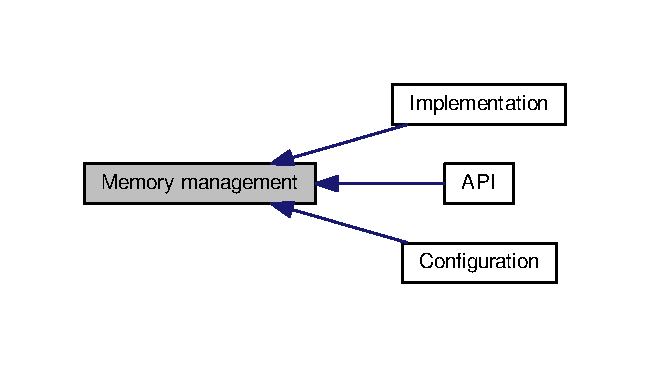
\includegraphics[width=312pt]{group__mem}
\end{center}
\end{figure}
\subsubsection*{Modules}
\begin{DoxyCompactItemize}
\item 
\hyperlink{group__mem__intf}{A\-P\-I}
\begin{DoxyCompactList}\small\item\em Memory Management A\-P\-I. \end{DoxyCompactList}\item 
\hyperlink{group__mem__cfg}{Configuration}
\item 
\hyperlink{group__mem__impl}{Implementation}
\end{DoxyCompactItemize}


\subsubsection{Detailed Description}
Memory Management overview. \hypertarget{group__mem_mem_index}{}\subsubsection{Sadrzaj}\label{group__mem_mem_index}

\begin{DoxyItemize}
\item \hyperlink{group__mem_mem_smem}{Staticki memorijski menadzer}
\item \hyperlink{group__mem_mem_dmem}{Dinamicki memorijski menadzer}
\item \hyperlink{group__mem_mem_pmem}{Pool memorijski menadzer}
\item \hyperlink{group__mem_mem_configuration}{Konfiguracija Memory Management modula}
\end{DoxyItemize}\hypertarget{group__mem_mem_smem}{}\subsubsection{Staticki memorijski menadzer}\label{group__mem_mem_smem}
Staticki memorijski menadzer moze samo da alocira memoriju i jednom alocirana memorija se ne moze osloboditi. Koristi se kada je potrebno staticki alocirati objekte koji se nikada ne brisu. Ovaj memorijski menadzer je najjednostavniji i najbrzi, pa se preporucuje za mikroprocesore sa ogranicenim performansama. Potrosnja memorije iznosi samo 4-\/8 bajtova za ceo memorijski menadzer i ne postoji dodatna potrosnja memorije prilikom alociranja.

Staticni memorijski menadzer je jedinstven za embedded sistem. Ne mogu postojati vise instanci staticnog alokatora. Velicina memorije koja se predaje staticnom alokatoru na koriscenje se podesava opcijom O\-P\-T\-\_\-\-M\-E\-M\-\_\-\-S\-M\-E\-M\-\_\-\-S\-I\-Z\-E.\hypertarget{group__mem_mem_dmem}{}\subsubsection{Dinamicki memorijski menadzer}\label{group__mem_mem_dmem}
Dinamicki memorijski menadzer je po funkcionalnosti identican sa funkcijama standardne C biblioteke malloc/free, sa tom izmenom da je prilagodjen za rad sa embedded sistemima.

Za razliku od staticnog alokatora, koji je jedinstven za sistem, u jednom embedded sistemu mogu postojati nekoliko instanci dinamickih alokatora. Razliciti dinamicki alokatori se referenciraju strukturom tipa \hyperlink{group__mem__intf_gacaaf771b18b3da8fa3b67a466390080e}{es\-D\-Mem\-Handle\-\_\-\-T}. Pogledati primer \hyperlink{dmem_two_buffs_8c-example}{dmem\-\_\-two\-\_\-buffs.\-c}.\hypertarget{group__mem_mem_ff_alloc}{}\paragraph{First Fit algoritam}\label{group__mem_mem_ff_alloc}
U ovom algoritmu, alokator cuva listu slobodnih blokova i po prijemu zahteva za memoriju, skenira duz liste za prvim blokom koji je dovoljno veliki da opsluzi zahtev. Ako je izabrani blok dovoljno veci nego sto je zahtevano onda se blok deli na dva dela, jedan deo se predaje korisniku, a drugi blok se postavlja nazad u listu slobodnih blokova. Kada se vrsi reciklaza blokova, najpre se proveravaju susedni blokovi da li su zauzeti. Susedni blokovi koji su slobodni spajaju se sa blokom koji se reciklira i na taj nacin formira novi, veci blok.\hypertarget{group__mem_mem_ff_specs}{}\paragraph{Specifikacije first fit alokatora}\label{group__mem_mem_ff_specs}

\begin{DoxyItemize}
\item Maksimalno vreme izvrsavanja operacije alokacije bloka {\bfseries nije} unapred poznato. Zbog navedene cinjenice alokator nije pogodan za hard real-\/time sisteme.
\item Maksimalno vreme izvrsavanja operacije dealokacije bloka je unapred poznato.
\item Ukupno minimalno zauzece R\-A\-M memorije (Cortex-\/\-M3 arch)\-: {\bfseries 28\-B} 
\end{DoxyItemize}\hypertarget{group__mem_mem_pmem}{}\subsubsection{Pool memorijski menadzer}\label{group__mem_mem_pmem}
Pool memorijski menadzer je vrlo slican dinamickom memorijskom menadzeru sa tom razlikom sto ne moze da se zatrazi proizvoljna kolicina memorije. Potrazivanje memorije se vrsi unapred definisanom velicinom bloka koja vazi za datu instancu pool memorije.

Podrzano je postojanje veceg broja razlicitih instanci, koje se referenciraju strukturama tipa \hyperlink{group__mem__intf_gaf82f01d26c4f6bc9a2b672a673b09ce2}{es\-P\-Mem\-Handle\-\_\-\-T}. Pogledati primer \hyperlink{pmem_two_buffs_8c-example}{pmem\-\_\-two\-\_\-buffs.\-c}.\hypertarget{group__mem_mem_pool_specs}{}\paragraph{Specifikacije pool alokatora}\label{group__mem_mem_pool_specs}

\begin{DoxyItemize}
\item Maksimalno vreme izvrsavanja operacije alokacije bloka {\bfseries je} unapred poznato. Zbog navedene cinjenice alokator {\bfseries je} pogodan za hard real-\/time sisteme.
\item Maksimalno vreme izvrsavanja operacije dealokacije bloka je unapred poznato.
\item Ukupno minimalno zauzece R\-A\-M memorije (Cortex-\/\-M3 arch)\-: {\bfseries 12\-B} 
\end{DoxyItemize}\hypertarget{group__mem_mem_configuration}{}\subsubsection{Konfiguracija Memory Management modula}\label{group__mem_mem_configuration}
Konfiguracija se vrsi u datoteci mem\-\_\-config.\-h. Navodjenje opcija se vrsi u sekciji D\-E\-F\-I\-N\-E\-S.

Na primer, ako je potrebno dodeliti 1024\-B memorije static alokatoru onda se u datoteci mem\-\_\-config.\-h u sekciji {\ttfamily {\bfseries D\-E\-F\-I\-N\-E\-S} unosi} sledece\-:


\begin{DoxyCode}
    :
    :
    
\textcolor{comment}{/*===============================================================  DEFINES  ==*/}
    
    :
    :
    
\textcolor{preprocessor}{#define OPT\_MEM\_SMEM\_SIZE               1024U}
\textcolor{preprocessor}{}
    :
    :
    
\textcolor{comment}{/*==============================================================  SETTINGS  ==*/},

    :
    :
\end{DoxyCode}


Za opcije Memory Management modula pogledati \hyperlink{group__mem__cfg}{Configuration}. 
\hypertarget{group__mem__intf}{\subsection{A\-P\-I}
\label{group__mem__intf}\index{A\-P\-I@{A\-P\-I}}
}


Memory Management A\-P\-I.  


Collaboration diagram for A\-P\-I\-:\nopagebreak
\begin{figure}[H]
\begin{center}
\leavevmode
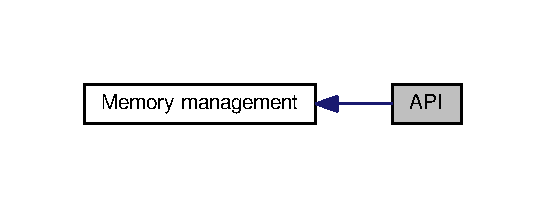
\includegraphics[width=262pt]{group__mem__intf}
\end{center}
\end{figure}
\subsubsection*{Data Structures}
\begin{DoxyCompactItemize}
\item 
struct \hyperlink{structesMemStatus}{es\-Mem\-Status}
\begin{DoxyCompactList}\small\item\em Memory status structure. \end{DoxyCompactList}\item 
struct \hyperlink{structesSMemHandle}{es\-S\-Mem\-Handle}
\begin{DoxyCompactList}\small\item\em Static memory instance handle structure. \end{DoxyCompactList}\item 
struct \hyperlink{structesPMemHandle}{es\-P\-Mem\-Handle}
\begin{DoxyCompactList}\small\item\em Pool memory instance handle structure. \end{DoxyCompactList}\item 
struct \hyperlink{structesDMemHandle}{es\-D\-Mem\-Handle}
\begin{DoxyCompactList}\small\item\em Dynamic memory instance handle structure. \end{DoxyCompactList}\end{DoxyCompactItemize}
\subsubsection*{Typedefs}
\begin{DoxyCompactItemize}
\item 
typedef struct \hyperlink{structesMemStatus}{es\-Mem\-Status} \hyperlink{group__mem__intf_ga0eb568b68247d93e2db804a681de0e9e}{es\-Mem\-Status\-\_\-\-T}
\begin{DoxyCompactList}\small\item\em Memory status type. \end{DoxyCompactList}\end{DoxyCompactItemize}
\subsubsection*{Static memory manager -\/ S\-Mem}
\begin{DoxyCompactItemize}
\item 
typedef struct \hyperlink{structesSMemHandle}{es\-S\-Mem\-Handle} \hyperlink{group__mem__intf_gabf19a317cc22713cfb45ae1e43d34d7e}{es\-S\-Mem\-Handle\-\_\-\-T}
\begin{DoxyCompactList}\small\item\em Static memory instance handle type. \end{DoxyCompactList}\end{DoxyCompactItemize}
\subsubsection*{Pool memory allocator -\/ P\-Mem}
\begin{DoxyCompactItemize}
\item 
typedef struct \hyperlink{structesPMemHandle}{es\-P\-Mem\-Handle} \hyperlink{group__mem__intf_gaf82f01d26c4f6bc9a2b672a673b09ce2}{es\-P\-Mem\-Handle\-\_\-\-T}
\begin{DoxyCompactList}\small\item\em Pool memory instance handle type. \end{DoxyCompactList}\end{DoxyCompactItemize}
\subsubsection*{Dynamic memory allocator -\/ D\-Mem}
\begin{DoxyCompactItemize}
\item 
typedef struct \hyperlink{structesDMemHandle}{es\-D\-Mem\-Handle} \hyperlink{group__mem__intf_gacaaf771b18b3da8fa3b67a466390080e}{es\-D\-Mem\-Handle\-\_\-\-T}
\begin{DoxyCompactList}\small\item\em Dynamic memory instance handle type. \end{DoxyCompactList}\end{DoxyCompactItemize}
\subsubsection*{Default memory instance handles}
\begin{DoxyCompactItemize}
\item 
\hyperlink{group__mem__intf_gabf19a317cc22713cfb45ae1e43d34d7e}{es\-S\-Mem\-Handle\-\_\-\-T} \hyperlink{group__mem__intf_ga59214c7e13470c5e76c7b59c4f084b1c}{Def\-S\-Mem\-Handle}
\begin{DoxyCompactList}\small\item\em Default static memory handle. \end{DoxyCompactList}\item 
\hyperlink{group__mem__intf_gaf82f01d26c4f6bc9a2b672a673b09ce2}{es\-P\-Mem\-Handle\-\_\-\-T} \hyperlink{group__mem__intf_gafb0dc701e9679157a617a091843bcd7f}{Def\-P\-Mem\-Handle}
\begin{DoxyCompactList}\small\item\em Default pool memory handle. \end{DoxyCompactList}\item 
\hyperlink{group__mem__intf_gacaaf771b18b3da8fa3b67a466390080e}{es\-D\-Mem\-Handle\-\_\-\-T} \hyperlink{group__mem__intf_gae2d3f8ca3b99ba0a5b9d9518a7bc280b}{Def\-D\-Mem\-Handle}
\begin{DoxyCompactList}\small\item\em Default dynamic memory handle. \end{DoxyCompactList}\end{DoxyCompactItemize}
\subsubsection*{Static memory manager}
\begin{DoxyCompactItemize}
\item 
void \hyperlink{group__mem__intf_ga53acef4ba27e5e401ac2e1f862e07a8b}{es\-S\-Mem\-Init} (\hyperlink{group__mem__intf_gabf19a317cc22713cfb45ae1e43d34d7e}{es\-S\-Mem\-Handle\-\_\-\-T} $\ast$handle, void $\ast$storage, size\-\_\-t storage\-Size)
\begin{DoxyCompactList}\small\item\em Initializes static memory instance. \end{DoxyCompactList}\item 
void $\ast$ \hyperlink{group__mem__intf_ga2e2086778aa0eb21156044730a1f380b}{es\-S\-Mem\-Alloc\-I} (\hyperlink{group__mem__intf_gabf19a317cc22713cfb45ae1e43d34d7e}{es\-S\-Mem\-Handle\-\_\-\-T} $\ast$handle, size\-\_\-t size)
\begin{DoxyCompactList}\small\item\em Allocates static memory of size {\ttfamily size}. \end{DoxyCompactList}\item 
void $\ast$ \hyperlink{group__mem__intf_ga23c0a40e0c40dabed8c22d9d65709c65}{es\-S\-Mem\-Alloc} (\hyperlink{group__mem__intf_gabf19a317cc22713cfb45ae1e43d34d7e}{es\-S\-Mem\-Handle\-\_\-\-T} $\ast$handle, size\-\_\-t size)
\begin{DoxyCompactList}\small\item\em Allocates static memory of size {\ttfamily size}. \end{DoxyCompactList}\item 
void \hyperlink{group__mem__intf_ga87b817ce71357521c4cd43a9cb587201}{es\-S\-Mem\-Update\-Status\-I} (\hyperlink{group__mem__intf_gabf19a317cc22713cfb45ae1e43d34d7e}{es\-S\-Mem\-Handle\-\_\-\-T} $\ast$handle, \hyperlink{group__mem__intf_ga0eb568b68247d93e2db804a681de0e9e}{es\-Mem\-Status\-\_\-\-T} $\ast$status)
\begin{DoxyCompactList}\small\item\em Returns various information about given memory instance. \end{DoxyCompactList}\item 
void \hyperlink{group__mem__intf_gac0ad18ef5c9332358a4d0a5ded270f34}{es\-S\-Mem\-Update\-Status} (\hyperlink{group__mem__intf_gabf19a317cc22713cfb45ae1e43d34d7e}{es\-S\-Mem\-Handle\-\_\-\-T} $\ast$handle, \hyperlink{group__mem__intf_ga0eb568b68247d93e2db804a681de0e9e}{es\-Mem\-Status\-\_\-\-T} $\ast$status)
\begin{DoxyCompactList}\small\item\em Returns various information about given memory instance. \end{DoxyCompactList}\end{DoxyCompactItemize}
\subsubsection*{Pool memory manager}
\begin{DoxyCompactItemize}
\item 
void \hyperlink{group__mem__intf_gac151cf4385488838b0507936e67e2584}{es\-P\-Mem\-Init} (\hyperlink{group__mem__intf_gaf82f01d26c4f6bc9a2b672a673b09ce2}{es\-P\-Mem\-Handle\-\_\-\-T} $\ast$handle, void $\ast$pool, size\-\_\-t pool\-Size, size\-\_\-t block\-Size)
\begin{DoxyCompactList}\small\item\em Initializes pool memory instance. \end{DoxyCompactList}\item 
size\-\_\-t \hyperlink{group__mem__intf_gab82743b6c82847c748bf5193f0f211ec}{es\-P\-Mem\-Calc\-Pool\-Size} (size\-\_\-t blocks, size\-\_\-t block\-Size)
\begin{DoxyCompactList}\small\item\em Calculates required reserved memory size for defined number of blocks. \end{DoxyCompactList}\item 
void $\ast$ \hyperlink{group__mem__intf_gabdacce602565fcd6a186c2834cb74488}{es\-P\-Mem\-Alloc\-I} (\hyperlink{group__mem__intf_gaf82f01d26c4f6bc9a2b672a673b09ce2}{es\-P\-Mem\-Handle\-\_\-\-T} $\ast$handle)
\begin{DoxyCompactList}\small\item\em Allocate one block from memory pool. \end{DoxyCompactList}\item 
void $\ast$ \hyperlink{group__mem__intf_gac750c9ec7780f5dc616e8a04a6668f34}{es\-P\-Mem\-Alloc} (\hyperlink{group__mem__intf_gaf82f01d26c4f6bc9a2b672a673b09ce2}{es\-P\-Mem\-Handle\-\_\-\-T} $\ast$handle)
\begin{DoxyCompactList}\small\item\em Allocate one block from memory pool. \end{DoxyCompactList}\item 
void \hyperlink{group__mem__intf_ga2c0f1b135c5639809b17dfe44e06f1b5}{es\-P\-Mem\-De\-Alloc\-I} (\hyperlink{group__mem__intf_gaf82f01d26c4f6bc9a2b672a673b09ce2}{es\-P\-Mem\-Handle\-\_\-\-T} $\ast$handle, void $\ast$mem)
\begin{DoxyCompactList}\small\item\em Oslobadja prethodno alocirani blok. \end{DoxyCompactList}\item 
void \hyperlink{group__mem__intf_gacd393e705fe5531cae380cc9b68f7a23}{es\-P\-Mem\-De\-Alloc} (\hyperlink{group__mem__intf_gaf82f01d26c4f6bc9a2b672a673b09ce2}{es\-P\-Mem\-Handle\-\_\-\-T} $\ast$handle, void $\ast$mem)
\begin{DoxyCompactList}\small\item\em Oslobadja prethodno alocirani blok. \end{DoxyCompactList}\item 
void \hyperlink{group__mem__intf_gab568f5b51f11f2bc315412c35bfc28e9}{es\-P\-Mem\-Update\-Status\-I} (\hyperlink{group__mem__intf_gaf82f01d26c4f6bc9a2b672a673b09ce2}{es\-P\-Mem\-Handle\-\_\-\-T} $\ast$handle, \hyperlink{group__mem__intf_ga0eb568b68247d93e2db804a681de0e9e}{es\-Mem\-Status\-\_\-\-T} $\ast$status)
\begin{DoxyCompactList}\small\item\em Vraca statusne informacije pool memorije. \end{DoxyCompactList}\item 
void \hyperlink{group__mem__intf_ga8148d4ad98ed5e9ecc04b7983433555e}{es\-P\-Mem\-Update\-Status} (\hyperlink{group__mem__intf_gaf82f01d26c4f6bc9a2b672a673b09ce2}{es\-P\-Mem\-Handle\-\_\-\-T} $\ast$handle, \hyperlink{group__mem__intf_ga0eb568b68247d93e2db804a681de0e9e}{es\-Mem\-Status\-\_\-\-T} $\ast$status)
\begin{DoxyCompactList}\small\item\em Vraca statusne informacije pool memorije. \end{DoxyCompactList}\end{DoxyCompactItemize}
\subsubsection*{Dynamic memory allocator}
\begin{DoxyCompactItemize}
\item 
void \hyperlink{group__mem__intf_ga10ef80121c0c742b9ad81f24eff91c7f}{es\-D\-Mem\-Init} (\hyperlink{group__mem__intf_gacaaf771b18b3da8fa3b67a466390080e}{es\-D\-Mem\-Handle\-\_\-\-T} $\ast$handle, void $\ast$storage, size\-\_\-t storage\-Size)
\begin{DoxyCompactList}\small\item\em Inicijalizuje dinamican memorijski alokator. \end{DoxyCompactList}\item 
void $\ast$ \hyperlink{group__mem__intf_ga807a7d2e705b1802b7671c0c903611a6}{es\-D\-Mem\-Alloc\-I} (\hyperlink{group__mem__intf_gacaaf771b18b3da8fa3b67a466390080e}{es\-D\-Mem\-Handle\-\_\-\-T} $\ast$handle, size\-\_\-t size)
\begin{DoxyCompactList}\small\item\em Dodeljuje memorijski prostor velicine {\ttfamily size}. \end{DoxyCompactList}\item 
void $\ast$ \hyperlink{group__mem__intf_ga7aa5c1f6bda178e4860f0727b1fd3590}{es\-D\-Mem\-Alloc} (\hyperlink{group__mem__intf_gacaaf771b18b3da8fa3b67a466390080e}{es\-D\-Mem\-Handle\-\_\-\-T} $\ast$handle, size\-\_\-t size)
\begin{DoxyCompactList}\small\item\em Dodeljuje memorijski prostor velicine {\ttfamily size}. \end{DoxyCompactList}\item 
void \hyperlink{group__mem__intf_gad56192526f2b6ec1f927d21b15e1bc11}{es\-D\-Mem\-De\-Alloc\-I} (\hyperlink{group__mem__intf_gacaaf771b18b3da8fa3b67a466390080e}{es\-D\-Mem\-Handle\-\_\-\-T} $\ast$handle, void $\ast$mem)
\begin{DoxyCompactList}\small\item\em Reciklira memorijski prostor na koji pokazije {\ttfamily mem} pokazivac. \end{DoxyCompactList}\item 
void \hyperlink{group__mem__intf_gad63c5b88aae0a4626763d934fdcdc9d1}{es\-D\-Mem\-De\-Alloc} (\hyperlink{group__mem__intf_gacaaf771b18b3da8fa3b67a466390080e}{es\-D\-Mem\-Handle\-\_\-\-T} $\ast$handle, void $\ast$mem)
\begin{DoxyCompactList}\small\item\em Reciklira memorijski prostor na koji pokazije {\ttfamily mem} pokazivac. \end{DoxyCompactList}\item 
void \hyperlink{group__mem__intf_gad1bddd779876d000f8906ec7ac747fa4}{es\-D\-Mem\-Update\-Status\-I} (\hyperlink{group__mem__intf_gacaaf771b18b3da8fa3b67a466390080e}{es\-D\-Mem\-Handle\-\_\-\-T} $\ast$handle, \hyperlink{group__mem__intf_ga0eb568b68247d93e2db804a681de0e9e}{es\-Mem\-Status\-\_\-\-T} $\ast$status)
\begin{DoxyCompactList}\small\item\em Vraca velicinu trenutno slobodne memorije u bajtovima. \end{DoxyCompactList}\item 
void \hyperlink{group__mem__intf_ga22ab58d97d2519dccf91220f029ac87f}{es\-D\-Mem\-Update\-Status} (\hyperlink{group__mem__intf_gacaaf771b18b3da8fa3b67a466390080e}{es\-D\-Mem\-Handle\-\_\-\-T} $\ast$handle, \hyperlink{group__mem__intf_ga0eb568b68247d93e2db804a681de0e9e}{es\-Mem\-Status\-\_\-\-T} $\ast$status)
\begin{DoxyCompactList}\small\item\em Vraca velicinu trenutno slobodne memorije u bajtovima. \end{DoxyCompactList}\end{DoxyCompactItemize}


\subsubsection{Detailed Description}
Memory Management A\-P\-I. This module implements three classes of memory managers\-:
\begin{DoxyItemize}
\item dynamic
\item pool
\item static For more details see \hyperlink{group__mem}{Memory management}. 
\end{DoxyItemize}

\subsubsection{Typedef Documentation}
\hypertarget{group__mem__intf_ga0eb568b68247d93e2db804a681de0e9e}{\index{A\-P\-I@{A\-P\-I}!es\-Mem\-Status\-\_\-\-T@{es\-Mem\-Status\-\_\-\-T}}
\index{es\-Mem\-Status\-\_\-\-T@{es\-Mem\-Status\-\_\-\-T}!API@{A\-P\-I}}
\paragraph[{es\-Mem\-Status\-\_\-\-T}]{\setlength{\rightskip}{0pt plus 5cm}typedef struct {\bf es\-Mem\-Status} {\bf es\-Mem\-Status\-\_\-\-T}}}\label{group__mem__intf_ga0eb568b68247d93e2db804a681de0e9e}


Memory status type. 

\begin{DoxyParagraph}{Object class\-:}
Regular {\bfseries A\-P\-I} object, this object is part of the application programming interface. 
\end{DoxyParagraph}
\hypertarget{group__mem__intf_gabf19a317cc22713cfb45ae1e43d34d7e}{\index{A\-P\-I@{A\-P\-I}!es\-S\-Mem\-Handle\-\_\-\-T@{es\-S\-Mem\-Handle\-\_\-\-T}}
\index{es\-S\-Mem\-Handle\-\_\-\-T@{es\-S\-Mem\-Handle\-\_\-\-T}!API@{A\-P\-I}}
\paragraph[{es\-S\-Mem\-Handle\-\_\-\-T}]{\setlength{\rightskip}{0pt plus 5cm}typedef struct {\bf es\-S\-Mem\-Handle} {\bf es\-S\-Mem\-Handle\-\_\-\-T}}}\label{group__mem__intf_gabf19a317cc22713cfb45ae1e43d34d7e}


Static memory instance handle type. 

\begin{DoxyParagraph}{Object class\-:}
Regular {\bfseries A\-P\-I} object, this object is part of the application programming interface. 
\end{DoxyParagraph}
\hypertarget{group__mem__intf_gaf82f01d26c4f6bc9a2b672a673b09ce2}{\index{A\-P\-I@{A\-P\-I}!es\-P\-Mem\-Handle\-\_\-\-T@{es\-P\-Mem\-Handle\-\_\-\-T}}
\index{es\-P\-Mem\-Handle\-\_\-\-T@{es\-P\-Mem\-Handle\-\_\-\-T}!API@{A\-P\-I}}
\paragraph[{es\-P\-Mem\-Handle\-\_\-\-T}]{\setlength{\rightskip}{0pt plus 5cm}typedef struct {\bf es\-P\-Mem\-Handle} {\bf es\-P\-Mem\-Handle\-\_\-\-T}}}\label{group__mem__intf_gaf82f01d26c4f6bc9a2b672a673b09ce2}


Pool memory instance handle type. 

\begin{DoxyParagraph}{Object class\-:}
Regular {\bfseries A\-P\-I} object, this object is part of the application programming interface. 
\end{DoxyParagraph}
\hypertarget{group__mem__intf_gacaaf771b18b3da8fa3b67a466390080e}{\index{A\-P\-I@{A\-P\-I}!es\-D\-Mem\-Handle\-\_\-\-T@{es\-D\-Mem\-Handle\-\_\-\-T}}
\index{es\-D\-Mem\-Handle\-\_\-\-T@{es\-D\-Mem\-Handle\-\_\-\-T}!API@{A\-P\-I}}
\paragraph[{es\-D\-Mem\-Handle\-\_\-\-T}]{\setlength{\rightskip}{0pt plus 5cm}typedef struct {\bf es\-D\-Mem\-Handle} {\bf es\-D\-Mem\-Handle\-\_\-\-T}}}\label{group__mem__intf_gacaaf771b18b3da8fa3b67a466390080e}


Dynamic memory instance handle type. 

\begin{DoxyParagraph}{Object class\-:}
Regular {\bfseries A\-P\-I} object, this object is part of the application programming interface. 
\end{DoxyParagraph}


\subsubsection{Function Documentation}
\hypertarget{group__mem__intf_ga53acef4ba27e5e401ac2e1f862e07a8b}{\index{A\-P\-I@{A\-P\-I}!es\-S\-Mem\-Init@{es\-S\-Mem\-Init}}
\index{es\-S\-Mem\-Init@{es\-S\-Mem\-Init}!API@{A\-P\-I}}
\paragraph[{es\-S\-Mem\-Init}]{\setlength{\rightskip}{0pt plus 5cm}void es\-S\-Mem\-Init (
\begin{DoxyParamCaption}
\item[{{\bf es\-S\-Mem\-Handle\-\_\-\-T} $\ast$}]{handle, }
\item[{void $\ast$}]{storage, }
\item[{size\-\_\-t}]{storage\-Size}
\end{DoxyParamCaption}
)}}\label{group__mem__intf_ga53acef4ba27e5e401ac2e1f862e07a8b}


Initializes static memory instance. 


\begin{DoxyParams}{Parameters}
{\em handle} & Pointer to handle type variable, see \hyperlink{group__mem__intf_gabf19a317cc22713cfb45ae1e43d34d7e}{es\-S\-Mem\-Handle\-\_\-\-T}. \\
\hline
{\em storage} & Storage memory reserved for static memory manager. \\
\hline
{\em storage\-Size} & Size of reserved memory expresses in bytes.\\
\hline
\end{DoxyParams}
This function shall be called before any other static memory management function. \begin{DoxyParagraph}{Object class\-:}
Regular {\bfseries A\-P\-I} object, this object is part of the application programming interface. 
\end{DoxyParagraph}
\begin{Desc}
\item[Examples\-: ]\par
\hyperlink{dmem_init2_8c-example}{dmem\-\_\-init2.\-c}, \hyperlink{dmem_two_buffs_8c-example}{dmem\-\_\-two\-\_\-buffs.\-c}, \hyperlink{pmem_init2_8c-example}{pmem\-\_\-init2.\-c}, and \hyperlink{pmem_init3_8c-example}{pmem\-\_\-init3.\-c}.\end{Desc}
\hypertarget{group__mem__intf_ga2e2086778aa0eb21156044730a1f380b}{\index{A\-P\-I@{A\-P\-I}!es\-S\-Mem\-Alloc\-I@{es\-S\-Mem\-Alloc\-I}}
\index{es\-S\-Mem\-Alloc\-I@{es\-S\-Mem\-Alloc\-I}!API@{A\-P\-I}}
\paragraph[{es\-S\-Mem\-Alloc\-I}]{\setlength{\rightskip}{0pt plus 5cm}void$\ast$ es\-S\-Mem\-Alloc\-I (
\begin{DoxyParamCaption}
\item[{{\bf es\-S\-Mem\-Handle\-\_\-\-T} $\ast$}]{handle, }
\item[{size\-\_\-t}]{size}
\end{DoxyParamCaption}
)}}\label{group__mem__intf_ga2e2086778aa0eb21156044730a1f380b}


Allocates static memory of size {\ttfamily size}. 


\begin{DoxyParams}{Parameters}
{\em handle} & Pointer to static memory instance, see \hyperlink{group__mem__intf_gabf19a317cc22713cfb45ae1e43d34d7e}{es\-S\-Mem\-Handle\-\_\-\-T}. \\
\hline
{\em size} & The size of requested memory in bytes. \\
\hline
\end{DoxyParams}
\begin{DoxyReturn}{Returns}
Pointer to free memory of requested size. 
\end{DoxyReturn}
\begin{DoxyParagraph}{Function class\-:}
{\bfseries I class}, Interrupt-\/lock A\-P\-I function, this function can be called only from interrupts locked code sections. 
\end{DoxyParagraph}
\begin{Desc}
\item[Examples\-: ]\par
\hyperlink{dmem_init2_8c-example}{dmem\-\_\-init2.\-c}, \hyperlink{dmem_two_buffs_8c-example}{dmem\-\_\-two\-\_\-buffs.\-c}, \hyperlink{pmem_init2_8c-example}{pmem\-\_\-init2.\-c}, and \hyperlink{pmem_init3_8c-example}{pmem\-\_\-init3.\-c}.\end{Desc}
\hypertarget{group__mem__intf_ga23c0a40e0c40dabed8c22d9d65709c65}{\index{A\-P\-I@{A\-P\-I}!es\-S\-Mem\-Alloc@{es\-S\-Mem\-Alloc}}
\index{es\-S\-Mem\-Alloc@{es\-S\-Mem\-Alloc}!API@{A\-P\-I}}
\paragraph[{es\-S\-Mem\-Alloc}]{\setlength{\rightskip}{0pt plus 5cm}void$\ast$ es\-S\-Mem\-Alloc (
\begin{DoxyParamCaption}
\item[{{\bf es\-S\-Mem\-Handle\-\_\-\-T} $\ast$}]{handle, }
\item[{size\-\_\-t}]{size}
\end{DoxyParamCaption}
)}}\label{group__mem__intf_ga23c0a40e0c40dabed8c22d9d65709c65}


Allocates static memory of size {\ttfamily size}. 


\begin{DoxyParams}{Parameters}
{\em handle} & Pointer to static memory instance, see \hyperlink{group__mem__intf_gabf19a317cc22713cfb45ae1e43d34d7e}{es\-S\-Mem\-Handle\-\_\-\-T}. \\
\hline
{\em size} & The size of requested memory in bytes. \\
\hline
\end{DoxyParams}
\begin{DoxyReturn}{Returns}
Pointer to free memory of requested size. 
\end{DoxyReturn}
\begin{DoxyParagraph}{Object class\-:}
Regular {\bfseries A\-P\-I} object, this object is part of the application programming interface. 
\end{DoxyParagraph}
\hypertarget{group__mem__intf_ga87b817ce71357521c4cd43a9cb587201}{\index{A\-P\-I@{A\-P\-I}!es\-S\-Mem\-Update\-Status\-I@{es\-S\-Mem\-Update\-Status\-I}}
\index{es\-S\-Mem\-Update\-Status\-I@{es\-S\-Mem\-Update\-Status\-I}!API@{A\-P\-I}}
\paragraph[{es\-S\-Mem\-Update\-Status\-I}]{\setlength{\rightskip}{0pt plus 5cm}void es\-S\-Mem\-Update\-Status\-I (
\begin{DoxyParamCaption}
\item[{{\bf es\-S\-Mem\-Handle\-\_\-\-T} $\ast$}]{handle, }
\item[{{\bf es\-Mem\-Status\-\_\-\-T} $\ast$}]{status}
\end{DoxyParamCaption}
)}}\label{group__mem__intf_ga87b817ce71357521c4cd43a9cb587201}


Returns various information about given memory instance. 


\begin{DoxyParams}{Parameters}
{\em handle} & Pointer to static memory instance, see \hyperlink{group__mem__intf_gabf19a317cc22713cfb45ae1e43d34d7e}{es\-S\-Mem\-Handle\-\_\-\-T}. \\
\hline
{\em status} & Pointer to memory status type, see \hyperlink{group__mem__intf_ga0eb568b68247d93e2db804a681de0e9e}{es\-Mem\-Status\-\_\-\-T}. \\
\hline
\end{DoxyParams}
\begin{DoxyParagraph}{Function class\-:}
{\bfseries I class}, Interrupt-\/lock A\-P\-I function, this function can be called only from interrupts locked code sections. 
\end{DoxyParagraph}
\hypertarget{group__mem__intf_gac0ad18ef5c9332358a4d0a5ded270f34}{\index{A\-P\-I@{A\-P\-I}!es\-S\-Mem\-Update\-Status@{es\-S\-Mem\-Update\-Status}}
\index{es\-S\-Mem\-Update\-Status@{es\-S\-Mem\-Update\-Status}!API@{A\-P\-I}}
\paragraph[{es\-S\-Mem\-Update\-Status}]{\setlength{\rightskip}{0pt plus 5cm}void es\-S\-Mem\-Update\-Status (
\begin{DoxyParamCaption}
\item[{{\bf es\-S\-Mem\-Handle\-\_\-\-T} $\ast$}]{handle, }
\item[{{\bf es\-Mem\-Status\-\_\-\-T} $\ast$}]{status}
\end{DoxyParamCaption}
)}}\label{group__mem__intf_gac0ad18ef5c9332358a4d0a5ded270f34}


Returns various information about given memory instance. 


\begin{DoxyParams}{Parameters}
{\em handle} & Pointer to static memory instance, see \hyperlink{group__mem__intf_gabf19a317cc22713cfb45ae1e43d34d7e}{es\-S\-Mem\-Handle\-\_\-\-T}. \\
\hline
{\em status} & Pointer to memory status type, see \hyperlink{group__mem__intf_ga0eb568b68247d93e2db804a681de0e9e}{es\-Mem\-Status\-\_\-\-T}. \\
\hline
\end{DoxyParams}
\begin{DoxyParagraph}{Object class\-:}
Regular {\bfseries A\-P\-I} object, this object is part of the application programming interface. 
\end{DoxyParagraph}
\hypertarget{group__mem__intf_gac151cf4385488838b0507936e67e2584}{\index{A\-P\-I@{A\-P\-I}!es\-P\-Mem\-Init@{es\-P\-Mem\-Init}}
\index{es\-P\-Mem\-Init@{es\-P\-Mem\-Init}!API@{A\-P\-I}}
\paragraph[{es\-P\-Mem\-Init}]{\setlength{\rightskip}{0pt plus 5cm}void es\-P\-Mem\-Init (
\begin{DoxyParamCaption}
\item[{{\bf es\-P\-Mem\-Handle\-\_\-\-T} $\ast$}]{handle, }
\item[{void $\ast$}]{pool, }
\item[{size\-\_\-t}]{pool\-Size, }
\item[{size\-\_\-t}]{block\-Size}
\end{DoxyParamCaption}
)}}\label{group__mem__intf_gac151cf4385488838b0507936e67e2584}


Initializes pool memory instance. 


\begin{DoxyParams}{Parameters}
{\em handle} & Pointer to pool memory instance, see \hyperlink{group__mem__intf_gaf82f01d26c4f6bc9a2b672a673b09ce2}{es\-P\-Mem\-Handle\-\_\-\-T}. \\
\hline
{\em pool} & Reserved memory area for pool allocator. \\
\hline
{\em pool\-Size} & The size of reserved memory area expressed in bytes. \\
\hline
{\em block\-Size} & The size of one block expressed in bytes.\\
\hline
\end{DoxyParams}
This function must be called before any call to \hyperlink{group__mem__intf_gabdacce602565fcd6a186c2834cb74488}{es\-P\-Mem\-Alloc\-I()} or \hyperlink{group__mem__intf_gac750c9ec7780f5dc616e8a04a6668f34}{es\-P\-Mem\-Alloc()}. \begin{DoxyWarning}{Warning}
Pointers to {\ttfamily handle} and {\ttfamily pool} must be aligned to C\-P\-U defined alignment. 
\end{DoxyWarning}
\begin{DoxyParagraph}{Object class\-:}
Regular {\bfseries A\-P\-I} object, this object is part of the application programming interface. 
\end{DoxyParagraph}
\begin{Desc}
\item[Examples\-: ]\par
\hyperlink{pmem_init1_8c-example}{pmem\-\_\-init1.\-c}, \hyperlink{pmem_init2_8c-example}{pmem\-\_\-init2.\-c}, \hyperlink{pmem_init3_8c-example}{pmem\-\_\-init3.\-c}, and \hyperlink{pmem_two_buffs_8c-example}{pmem\-\_\-two\-\_\-buffs.\-c}.\end{Desc}
\hypertarget{group__mem__intf_gab82743b6c82847c748bf5193f0f211ec}{\index{A\-P\-I@{A\-P\-I}!es\-P\-Mem\-Calc\-Pool\-Size@{es\-P\-Mem\-Calc\-Pool\-Size}}
\index{es\-P\-Mem\-Calc\-Pool\-Size@{es\-P\-Mem\-Calc\-Pool\-Size}!API@{A\-P\-I}}
\paragraph[{es\-P\-Mem\-Calc\-Pool\-Size}]{\setlength{\rightskip}{0pt plus 5cm}size\-\_\-t es\-P\-Mem\-Calc\-Pool\-Size (
\begin{DoxyParamCaption}
\item[{size\-\_\-t}]{blocks, }
\item[{size\-\_\-t}]{block\-Size}
\end{DoxyParamCaption}
)}}\label{group__mem__intf_gab82743b6c82847c748bf5193f0f211ec}


Calculates required reserved memory size for defined number of blocks. 


\begin{DoxyParams}{Parameters}
{\em blocks} & Number of required blocks. \\
\hline
{\em block\-Size} & The size of one block. \\
\hline
\end{DoxyParams}
\begin{DoxyReturn}{Returns}
Required reserved memory size. 
\end{DoxyReturn}
\begin{DoxyParagraph}{Object class\-:}
Regular {\bfseries A\-P\-I} object, this object is part of the application programming interface. 
\end{DoxyParagraph}
\begin{Desc}
\item[Examples\-: ]\par
\hyperlink{pmem_init3_8c-example}{pmem\-\_\-init3.\-c}.\end{Desc}
\hypertarget{group__mem__intf_gabdacce602565fcd6a186c2834cb74488}{\index{A\-P\-I@{A\-P\-I}!es\-P\-Mem\-Alloc\-I@{es\-P\-Mem\-Alloc\-I}}
\index{es\-P\-Mem\-Alloc\-I@{es\-P\-Mem\-Alloc\-I}!API@{A\-P\-I}}
\paragraph[{es\-P\-Mem\-Alloc\-I}]{\setlength{\rightskip}{0pt plus 5cm}void$\ast$ es\-P\-Mem\-Alloc\-I (
\begin{DoxyParamCaption}
\item[{{\bf es\-P\-Mem\-Handle\-\_\-\-T} $\ast$}]{handle}
\end{DoxyParamCaption}
)}}\label{group__mem__intf_gabdacce602565fcd6a186c2834cb74488}


Allocate one block from memory pool. 


\begin{DoxyParams}{Parameters}
{\em handle} & Pointer to pool memory instance, see \hyperlink{group__mem__intf_gaf82f01d26c4f6bc9a2b672a673b09ce2}{es\-P\-Mem\-Handle\-\_\-\-T}. \\
\hline
\end{DoxyParams}
\begin{DoxyReturn}{Returns}
Pointer to requested block. 
\end{DoxyReturn}
\begin{DoxyParagraph}{Function class\-:}
{\bfseries I class}, Interrupt-\/lock A\-P\-I function, this function can be called only from interrupts locked code sections. 
\end{DoxyParagraph}
\begin{Desc}
\item[Examples\-: ]\par
\hyperlink{pmem_init1_8c-example}{pmem\-\_\-init1.\-c}, \hyperlink{pmem_init2_8c-example}{pmem\-\_\-init2.\-c}, \hyperlink{pmem_init3_8c-example}{pmem\-\_\-init3.\-c}, and \hyperlink{pmem_two_buffs_8c-example}{pmem\-\_\-two\-\_\-buffs.\-c}.\end{Desc}
\hypertarget{group__mem__intf_gac750c9ec7780f5dc616e8a04a6668f34}{\index{A\-P\-I@{A\-P\-I}!es\-P\-Mem\-Alloc@{es\-P\-Mem\-Alloc}}
\index{es\-P\-Mem\-Alloc@{es\-P\-Mem\-Alloc}!API@{A\-P\-I}}
\paragraph[{es\-P\-Mem\-Alloc}]{\setlength{\rightskip}{0pt plus 5cm}void$\ast$ es\-P\-Mem\-Alloc (
\begin{DoxyParamCaption}
\item[{{\bf es\-P\-Mem\-Handle\-\_\-\-T} $\ast$}]{handle}
\end{DoxyParamCaption}
)}}\label{group__mem__intf_gac750c9ec7780f5dc616e8a04a6668f34}


Allocate one block from memory pool. 


\begin{DoxyParams}{Parameters}
{\em handle} & Pointer to pool memory instance, see \hyperlink{group__mem__intf_gaf82f01d26c4f6bc9a2b672a673b09ce2}{es\-P\-Mem\-Handle\-\_\-\-T}. \\
\hline
\end{DoxyParams}
\begin{DoxyReturn}{Returns}
Pointer to requested block. 
\end{DoxyReturn}
\begin{DoxyParagraph}{Object class\-:}
Regular {\bfseries A\-P\-I} object, this object is part of the application programming interface. 
\end{DoxyParagraph}
\hypertarget{group__mem__intf_ga2c0f1b135c5639809b17dfe44e06f1b5}{\index{A\-P\-I@{A\-P\-I}!es\-P\-Mem\-De\-Alloc\-I@{es\-P\-Mem\-De\-Alloc\-I}}
\index{es\-P\-Mem\-De\-Alloc\-I@{es\-P\-Mem\-De\-Alloc\-I}!API@{A\-P\-I}}
\paragraph[{es\-P\-Mem\-De\-Alloc\-I}]{\setlength{\rightskip}{0pt plus 5cm}void es\-P\-Mem\-De\-Alloc\-I (
\begin{DoxyParamCaption}
\item[{{\bf es\-P\-Mem\-Handle\-\_\-\-T} $\ast$}]{handle, }
\item[{void $\ast$}]{mem}
\end{DoxyParamCaption}
)}}\label{group__mem__intf_ga2c0f1b135c5639809b17dfe44e06f1b5}


Oslobadja prethodno alocirani blok. 


\begin{DoxyParams}[1]{Parameters}
\mbox{\tt in}  & {\em handle} & Deskriptor pool alokatora \\
\hline
\mbox{\tt in}  & {\em mem} & Prethodno alociran blok memorije \\
\hline
\end{DoxyParams}
\begin{DoxyParagraph}{Function class\-:}
{\bfseries I class}, Interrupt-\/lock A\-P\-I function, this function can be called only from interrupts locked code sections. 
\end{DoxyParagraph}
\begin{Desc}
\item[Examples\-: ]\par
\hyperlink{pmem_init1_8c-example}{pmem\-\_\-init1.\-c}, \hyperlink{pmem_init2_8c-example}{pmem\-\_\-init2.\-c}, \hyperlink{pmem_init3_8c-example}{pmem\-\_\-init3.\-c}, and \hyperlink{pmem_two_buffs_8c-example}{pmem\-\_\-two\-\_\-buffs.\-c}.\end{Desc}
\hypertarget{group__mem__intf_gacd393e705fe5531cae380cc9b68f7a23}{\index{A\-P\-I@{A\-P\-I}!es\-P\-Mem\-De\-Alloc@{es\-P\-Mem\-De\-Alloc}}
\index{es\-P\-Mem\-De\-Alloc@{es\-P\-Mem\-De\-Alloc}!API@{A\-P\-I}}
\paragraph[{es\-P\-Mem\-De\-Alloc}]{\setlength{\rightskip}{0pt plus 5cm}void es\-P\-Mem\-De\-Alloc (
\begin{DoxyParamCaption}
\item[{{\bf es\-P\-Mem\-Handle\-\_\-\-T} $\ast$}]{handle, }
\item[{void $\ast$}]{mem}
\end{DoxyParamCaption}
)}}\label{group__mem__intf_gacd393e705fe5531cae380cc9b68f7a23}


Oslobadja prethodno alocirani blok. 


\begin{DoxyParams}[1]{Parameters}
\mbox{\tt in}  & {\em handle} & Deskriptor pool alokatora \\
\hline
\mbox{\tt in}  & {\em mem} & Prethodno alociran blok memorije \\
\hline
\end{DoxyParams}
\begin{DoxyNote}{Note}
Funkcija koristi makroe O\-P\-T\-\_\-\-G\-U\-A\-R\-D\-\_\-\-L\-O\-C\-K i O\-P\-T\-\_\-\-G\-U\-A\-R\-D\-\_\-\-U\-N\-L\-O\-C\-K za zastitu memorije od istovremenog pristupa. 
\end{DoxyNote}
\begin{DoxyParagraph}{Object class\-:}
Regular {\bfseries A\-P\-I} object, this object is part of the application programming interface. 
\end{DoxyParagraph}
\hypertarget{group__mem__intf_gab568f5b51f11f2bc315412c35bfc28e9}{\index{A\-P\-I@{A\-P\-I}!es\-P\-Mem\-Update\-Status\-I@{es\-P\-Mem\-Update\-Status\-I}}
\index{es\-P\-Mem\-Update\-Status\-I@{es\-P\-Mem\-Update\-Status\-I}!API@{A\-P\-I}}
\paragraph[{es\-P\-Mem\-Update\-Status\-I}]{\setlength{\rightskip}{0pt plus 5cm}void es\-P\-Mem\-Update\-Status\-I (
\begin{DoxyParamCaption}
\item[{{\bf es\-P\-Mem\-Handle\-\_\-\-T} $\ast$}]{handle, }
\item[{{\bf es\-Mem\-Status\-\_\-\-T} $\ast$}]{status}
\end{DoxyParamCaption}
)}}\label{group__mem__intf_gab568f5b51f11f2bc315412c35bfc28e9}


Vraca statusne informacije pool memorije. 


\begin{DoxyParams}[1]{Parameters}
\mbox{\tt in}  & {\em handle} & Deskriptor pool alokatora \\
\hline
\mbox{\tt out}  & {\em status} & Status struktura pool alokatora \\
\hline
\end{DoxyParams}
\begin{DoxyParagraph}{Function class\-:}
{\bfseries I class}, Interrupt-\/lock A\-P\-I function, this function can be called only from interrupts locked code sections. 
\end{DoxyParagraph}
\hypertarget{group__mem__intf_ga8148d4ad98ed5e9ecc04b7983433555e}{\index{A\-P\-I@{A\-P\-I}!es\-P\-Mem\-Update\-Status@{es\-P\-Mem\-Update\-Status}}
\index{es\-P\-Mem\-Update\-Status@{es\-P\-Mem\-Update\-Status}!API@{A\-P\-I}}
\paragraph[{es\-P\-Mem\-Update\-Status}]{\setlength{\rightskip}{0pt plus 5cm}void es\-P\-Mem\-Update\-Status (
\begin{DoxyParamCaption}
\item[{{\bf es\-P\-Mem\-Handle\-\_\-\-T} $\ast$}]{handle, }
\item[{{\bf es\-Mem\-Status\-\_\-\-T} $\ast$}]{status}
\end{DoxyParamCaption}
)}}\label{group__mem__intf_ga8148d4ad98ed5e9ecc04b7983433555e}


Vraca statusne informacije pool memorije. 


\begin{DoxyParams}[1]{Parameters}
\mbox{\tt in}  & {\em handle} & Deskriptor pool alokatora \\
\hline
\mbox{\tt out}  & {\em status} & Status struktura pool alokatora \\
\hline
\end{DoxyParams}
\begin{DoxyParagraph}{Object class\-:}
Regular {\bfseries A\-P\-I} object, this object is part of the application programming interface. 
\end{DoxyParagraph}
\hypertarget{group__mem__intf_ga10ef80121c0c742b9ad81f24eff91c7f}{\index{A\-P\-I@{A\-P\-I}!es\-D\-Mem\-Init@{es\-D\-Mem\-Init}}
\index{es\-D\-Mem\-Init@{es\-D\-Mem\-Init}!API@{A\-P\-I}}
\paragraph[{es\-D\-Mem\-Init}]{\setlength{\rightskip}{0pt plus 5cm}void es\-D\-Mem\-Init (
\begin{DoxyParamCaption}
\item[{{\bf es\-D\-Mem\-Handle\-\_\-\-T} $\ast$}]{handle, }
\item[{void $\ast$}]{storage, }
\item[{size\-\_\-t}]{storage\-Size}
\end{DoxyParamCaption}
)}}\label{group__mem__intf_ga10ef80121c0c742b9ad81f24eff91c7f}


Inicijalizuje dinamican memorijski alokator. 


\begin{DoxyParams}[1]{Parameters}
\mbox{\tt out}  & {\em handle} & Deskriptor dinamickog alokatora \\
\hline
\mbox{\tt in}  & {\em storage} & Predefinisani memorijski prostor koji se predaje dinamickom alokatoru na koriscenje \\
\hline
 & {\em storage\-Size} & Velicina memorijskog prostora u bajtovima\\
\hline
\end{DoxyParams}
Ova funkcija se mora pozvati pre koriscenja funkcija dinamickog memorijskog alokatora. \begin{DoxyWarning}{Warning}
Funkcija zahteva da pokazivaci handle i pool budu poravnani (aligned). Ukoliko se koriste e\-Solid alokatori za instaciranje {\ttfamily handle} strukture i {\ttfamily pool\-Storage} onda je poravnani pristup osiguran. 

Funkcija zahteva da velicina memorijskog prostora {\ttfamily storage\-Size} bude poravnana (aligned). Na primer za 32-\/bitni procesor (poravnanje 4 bajta)\-: ako je {\ttfamily storage\-Size} == 313 onda je potrebno poravnati na sledecu vecu vrednost koja je deljiva sa 4, u ovom slucaju ce to biti 316. 
\end{DoxyWarning}
\begin{DoxyParagraph}{Object class\-:}
Regular {\bfseries A\-P\-I} object, this object is part of the application programming interface. 
\end{DoxyParagraph}
\begin{Desc}
\item[Examples\-: ]\par
\hyperlink{dmem_init1_8c-example}{dmem\-\_\-init1.\-c}, \hyperlink{dmem_init2_8c-example}{dmem\-\_\-init2.\-c}, and \hyperlink{dmem_two_buffs_8c-example}{dmem\-\_\-two\-\_\-buffs.\-c}.\end{Desc}
\hypertarget{group__mem__intf_ga807a7d2e705b1802b7671c0c903611a6}{\index{A\-P\-I@{A\-P\-I}!es\-D\-Mem\-Alloc\-I@{es\-D\-Mem\-Alloc\-I}}
\index{es\-D\-Mem\-Alloc\-I@{es\-D\-Mem\-Alloc\-I}!API@{A\-P\-I}}
\paragraph[{es\-D\-Mem\-Alloc\-I}]{\setlength{\rightskip}{0pt plus 5cm}void$\ast$ es\-D\-Mem\-Alloc\-I (
\begin{DoxyParamCaption}
\item[{{\bf es\-D\-Mem\-Handle\-\_\-\-T} $\ast$}]{handle, }
\item[{size\-\_\-t}]{size}
\end{DoxyParamCaption}
)}}\label{group__mem__intf_ga807a7d2e705b1802b7671c0c903611a6}


Dodeljuje memorijski prostor velicine {\ttfamily size}. 


\begin{DoxyParams}[1]{Parameters}
\mbox{\tt in}  & {\em handle} & Deskriptor dinamickog alokatora \\
\hline
 & {\em size} & Velicina zahtevanog memorijskog prostora u bajtovima. \\
\hline
\end{DoxyParams}
\begin{DoxyReturn}{Returns}
Pokazivac na rezervisani memorijski blok.
\end{DoxyReturn}
U debug rezimu ova funkcija uvek vraca pokazivac, odnosno, ne moze se desiti da vrati N\-U\-L\-L pokazivac, kao sto nalaze standardna implementacija {\ttfamily malloc} C funkcije. Ukoliko se zahtevana memorija ne moze dobaviti generisace se A\-S\-S\-E\-R\-T greska. Kada se ne koristi debug rezim funkcija se ponasa u skladu sa standardom. \begin{DoxyParagraph}{Function class\-:}
{\bfseries I class}, Interrupt-\/lock A\-P\-I function, this function can be called only from interrupts locked code sections. 
\end{DoxyParagraph}
\begin{Desc}
\item[Examples\-: ]\par
\hyperlink{dmem_init1_8c-example}{dmem\-\_\-init1.\-c}, \hyperlink{dmem_init2_8c-example}{dmem\-\_\-init2.\-c}, and \hyperlink{dmem_two_buffs_8c-example}{dmem\-\_\-two\-\_\-buffs.\-c}.\end{Desc}
\hypertarget{group__mem__intf_ga7aa5c1f6bda178e4860f0727b1fd3590}{\index{A\-P\-I@{A\-P\-I}!es\-D\-Mem\-Alloc@{es\-D\-Mem\-Alloc}}
\index{es\-D\-Mem\-Alloc@{es\-D\-Mem\-Alloc}!API@{A\-P\-I}}
\paragraph[{es\-D\-Mem\-Alloc}]{\setlength{\rightskip}{0pt plus 5cm}void$\ast$ es\-D\-Mem\-Alloc (
\begin{DoxyParamCaption}
\item[{{\bf es\-D\-Mem\-Handle\-\_\-\-T} $\ast$}]{handle, }
\item[{size\-\_\-t}]{size}
\end{DoxyParamCaption}
)}}\label{group__mem__intf_ga7aa5c1f6bda178e4860f0727b1fd3590}


Dodeljuje memorijski prostor velicine {\ttfamily size}. 


\begin{DoxyParams}[1]{Parameters}
\mbox{\tt in}  & {\em handle} & Deskriptor dinamickog alokatora \\
\hline
 & {\em size} & Velicina zahtevanog memorijskog prostora u bajtovima. \\
\hline
\end{DoxyParams}
\begin{DoxyReturn}{Returns}
Pokazivac na rezervisani memorijski blok.
\end{DoxyReturn}
U debug rezimu ova funkcija uvek vraca pokazivac, odnosno, ne moze se desiti da vrati N\-U\-L\-L pokazivac, kao sto nalaze standardna implementacija {\ttfamily malloc} C funkcije. Ukoliko se zahtevana memorija ne moze dobaviti generisace se A\-S\-S\-E\-R\-T greska. Kada se ne koristi debug rezim funkcija se ponasa u skladu sa standardom. \begin{DoxyNote}{Note}
Funkcija koristi makroe O\-P\-T\-\_\-\-G\-U\-A\-R\-D\-\_\-\-L\-O\-C\-K i O\-P\-T\-\_\-\-G\-U\-A\-R\-D\-\_\-\-U\-N\-L\-O\-C\-K za zastitu memorije od istovremenog pristupa. 
\end{DoxyNote}
\begin{DoxyParagraph}{Object class\-:}
Regular {\bfseries A\-P\-I} object, this object is part of the application programming interface. 
\end{DoxyParagraph}
\hypertarget{group__mem__intf_gad56192526f2b6ec1f927d21b15e1bc11}{\index{A\-P\-I@{A\-P\-I}!es\-D\-Mem\-De\-Alloc\-I@{es\-D\-Mem\-De\-Alloc\-I}}
\index{es\-D\-Mem\-De\-Alloc\-I@{es\-D\-Mem\-De\-Alloc\-I}!API@{A\-P\-I}}
\paragraph[{es\-D\-Mem\-De\-Alloc\-I}]{\setlength{\rightskip}{0pt plus 5cm}void es\-D\-Mem\-De\-Alloc\-I (
\begin{DoxyParamCaption}
\item[{{\bf es\-D\-Mem\-Handle\-\_\-\-T} $\ast$}]{handle, }
\item[{void $\ast$}]{mem}
\end{DoxyParamCaption}
)}}\label{group__mem__intf_gad56192526f2b6ec1f927d21b15e1bc11}


Reciklira memorijski prostor na koji pokazije {\ttfamily mem} pokazivac. 


\begin{DoxyParams}[1]{Parameters}
\mbox{\tt in}  & {\em handle} & Deskriptor dinamickog alokatora \\
\hline
\mbox{\tt in}  & {\em mem} & Pokazivac na prethodno dodeljen memorijski prostor. \\
\hline
\end{DoxyParams}
\begin{DoxyParagraph}{Function class\-:}
{\bfseries I class}, Interrupt-\/lock A\-P\-I function, this function can be called only from interrupts locked code sections. 
\end{DoxyParagraph}
\begin{Desc}
\item[Examples\-: ]\par
\hyperlink{dmem_init1_8c-example}{dmem\-\_\-init1.\-c}, \hyperlink{dmem_init2_8c-example}{dmem\-\_\-init2.\-c}, and \hyperlink{dmem_two_buffs_8c-example}{dmem\-\_\-two\-\_\-buffs.\-c}.\end{Desc}
\hypertarget{group__mem__intf_gad63c5b88aae0a4626763d934fdcdc9d1}{\index{A\-P\-I@{A\-P\-I}!es\-D\-Mem\-De\-Alloc@{es\-D\-Mem\-De\-Alloc}}
\index{es\-D\-Mem\-De\-Alloc@{es\-D\-Mem\-De\-Alloc}!API@{A\-P\-I}}
\paragraph[{es\-D\-Mem\-De\-Alloc}]{\setlength{\rightskip}{0pt plus 5cm}void es\-D\-Mem\-De\-Alloc (
\begin{DoxyParamCaption}
\item[{{\bf es\-D\-Mem\-Handle\-\_\-\-T} $\ast$}]{handle, }
\item[{void $\ast$}]{mem}
\end{DoxyParamCaption}
)}}\label{group__mem__intf_gad63c5b88aae0a4626763d934fdcdc9d1}


Reciklira memorijski prostor na koji pokazije {\ttfamily mem} pokazivac. 


\begin{DoxyParams}[1]{Parameters}
\mbox{\tt in}  & {\em handle} & Deskriptor dinamickog alokatora \\
\hline
\mbox{\tt in}  & {\em mem} & Pokazivac na prethodno dodeljen memorijski prostor. \\
\hline
\end{DoxyParams}
\begin{DoxyNote}{Note}
Funkcija koristi makroe O\-P\-T\-\_\-\-G\-U\-A\-R\-D\-\_\-\-L\-O\-C\-K i O\-P\-T\-\_\-\-G\-U\-A\-R\-D\-\_\-\-U\-N\-L\-O\-C\-K za zastitu memorije od istovremenog pristupa. 
\end{DoxyNote}
\begin{DoxyParagraph}{Object class\-:}
Regular {\bfseries A\-P\-I} object, this object is part of the application programming interface. 
\end{DoxyParagraph}
\hypertarget{group__mem__intf_gad1bddd779876d000f8906ec7ac747fa4}{\index{A\-P\-I@{A\-P\-I}!es\-D\-Mem\-Update\-Status\-I@{es\-D\-Mem\-Update\-Status\-I}}
\index{es\-D\-Mem\-Update\-Status\-I@{es\-D\-Mem\-Update\-Status\-I}!API@{A\-P\-I}}
\paragraph[{es\-D\-Mem\-Update\-Status\-I}]{\setlength{\rightskip}{0pt plus 5cm}void es\-D\-Mem\-Update\-Status\-I (
\begin{DoxyParamCaption}
\item[{{\bf es\-D\-Mem\-Handle\-\_\-\-T} $\ast$}]{handle, }
\item[{{\bf es\-Mem\-Status\-\_\-\-T} $\ast$}]{status}
\end{DoxyParamCaption}
)}}\label{group__mem__intf_gad1bddd779876d000f8906ec7ac747fa4}


Vraca velicinu trenutno slobodne memorije u bajtovima. 


\begin{DoxyParams}[1]{Parameters}
\mbox{\tt in}  & {\em handle} & Deskriptor dinamickog alokatora \\
\hline
\mbox{\tt out}  & {\em status} & Status struktura dinamickog alokatora\\
\hline
\end{DoxyParams}
Ukoliko je memorija jako fragmenitisana, sto je karakteristicno za first fir algoritam, moze se desiti da postoji dovoljno slobodne memorije, ali ne i bloka zahtevane velicine. U tom slucaju memorijski alokator nece biti u mogucnosti da ispuni zahtev. \begin{DoxyParagraph}{Function class\-:}
{\bfseries I class}, Interrupt-\/lock A\-P\-I function, this function can be called only from interrupts locked code sections. 
\end{DoxyParagraph}
\hypertarget{group__mem__intf_ga22ab58d97d2519dccf91220f029ac87f}{\index{A\-P\-I@{A\-P\-I}!es\-D\-Mem\-Update\-Status@{es\-D\-Mem\-Update\-Status}}
\index{es\-D\-Mem\-Update\-Status@{es\-D\-Mem\-Update\-Status}!API@{A\-P\-I}}
\paragraph[{es\-D\-Mem\-Update\-Status}]{\setlength{\rightskip}{0pt plus 5cm}void es\-D\-Mem\-Update\-Status (
\begin{DoxyParamCaption}
\item[{{\bf es\-D\-Mem\-Handle\-\_\-\-T} $\ast$}]{handle, }
\item[{{\bf es\-Mem\-Status\-\_\-\-T} $\ast$}]{status}
\end{DoxyParamCaption}
)}}\label{group__mem__intf_ga22ab58d97d2519dccf91220f029ac87f}


Vraca velicinu trenutno slobodne memorije u bajtovima. 


\begin{DoxyParams}[1]{Parameters}
\mbox{\tt in}  & {\em handle} & Deskriptor dinamickog alokatora \\
\hline
\mbox{\tt out}  & {\em status} & Status struktura dinamickog alokatora\\
\hline
\end{DoxyParams}
Ukoliko je memorija jako fragmenitisana, sto je karakteristicno za first fir algoritam, moze se desiti da postoji dovoljno slobodne memorije, ali ne i bloka zahtevane velicine. U tom slucaju memorijski alokator nece biti u mogucnosti da ispuni zahtev. \begin{DoxyParagraph}{Object class\-:}
Regular {\bfseries A\-P\-I} object, this object is part of the application programming interface. 
\end{DoxyParagraph}


\subsubsection{Variable Documentation}
\hypertarget{group__mem__intf_ga59214c7e13470c5e76c7b59c4f084b1c}{\index{A\-P\-I@{A\-P\-I}!Def\-S\-Mem\-Handle@{Def\-S\-Mem\-Handle}}
\index{Def\-S\-Mem\-Handle@{Def\-S\-Mem\-Handle}!API@{A\-P\-I}}
\paragraph[{Def\-S\-Mem\-Handle}]{\setlength{\rightskip}{0pt plus 5cm}{\bf es\-S\-Mem\-Handle\-\_\-\-T} Def\-S\-Mem\-Handle}}\label{group__mem__intf_ga59214c7e13470c5e76c7b59c4f084b1c}


Default static memory handle. 

\begin{DoxyParagraph}{Object class\-:}
Regular {\bfseries A\-P\-I} object, this object is part of the application programming interface. 
\end{DoxyParagraph}
\hypertarget{group__mem__intf_gafb0dc701e9679157a617a091843bcd7f}{\index{A\-P\-I@{A\-P\-I}!Def\-P\-Mem\-Handle@{Def\-P\-Mem\-Handle}}
\index{Def\-P\-Mem\-Handle@{Def\-P\-Mem\-Handle}!API@{A\-P\-I}}
\paragraph[{Def\-P\-Mem\-Handle}]{\setlength{\rightskip}{0pt plus 5cm}{\bf es\-P\-Mem\-Handle\-\_\-\-T} Def\-P\-Mem\-Handle}}\label{group__mem__intf_gafb0dc701e9679157a617a091843bcd7f}


Default pool memory handle. 

\begin{DoxyParagraph}{Object class\-:}
Regular {\bfseries A\-P\-I} object, this object is part of the application programming interface. 
\end{DoxyParagraph}
\hypertarget{group__mem__intf_gae2d3f8ca3b99ba0a5b9d9518a7bc280b}{\index{A\-P\-I@{A\-P\-I}!Def\-D\-Mem\-Handle@{Def\-D\-Mem\-Handle}}
\index{Def\-D\-Mem\-Handle@{Def\-D\-Mem\-Handle}!API@{A\-P\-I}}
\paragraph[{Def\-D\-Mem\-Handle}]{\setlength{\rightskip}{0pt plus 5cm}{\bf es\-D\-Mem\-Handle\-\_\-\-T} Def\-D\-Mem\-Handle}}\label{group__mem__intf_gae2d3f8ca3b99ba0a5b9d9518a7bc280b}


Default dynamic memory handle. 

\begin{DoxyParagraph}{Object class\-:}
Regular {\bfseries A\-P\-I} object, this object is part of the application programming interface. 
\end{DoxyParagraph}

\hypertarget{group__mem__impl}{\subsection{Implementation}
\label{group__mem__impl}\index{Implementation@{Implementation}}
}
Collaboration diagram for Implementation\-:\nopagebreak
\begin{figure}[H]
\begin{center}
\leavevmode
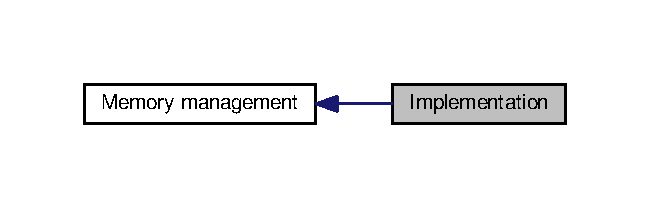
\includegraphics[width=312pt]{group__mem__impl}
\end{center}
\end{figure}
\subsubsection*{Data Structures}
\begin{DoxyCompactItemize}
\item 
struct \hyperlink{structpMemBlock}{p\-Mem\-Block}
\begin{DoxyCompactList}\small\item\em Pool allocator header structure. \end{DoxyCompactList}\end{DoxyCompactItemize}
\subsubsection*{Macros}
\begin{DoxyCompactItemize}
\item 
\#define \hyperlink{group__mem__impl_gae0fa2c7ba98034d2b0a59299edc64c66}{S\-M\-E\-M\-\_\-\-S\-I\-G\-N\-A\-T\-U\-R\-E}~((port\-Reg\-\_\-\-T)0x\-D\-E\-A\-D\-B\-E\-E\-D\-U)
\begin{DoxyCompactList}\small\item\em Signature for static memory manager. \end{DoxyCompactList}\item 
\#define \hyperlink{group__mem__impl_ga37e53ccf6c132baa9a610318a18c312e}{P\-M\-E\-M\-\_\-\-S\-I\-G\-N\-A\-T\-U\-R\-E}~((port\-Reg\-\_\-\-T)0x\-D\-E\-A\-D\-B\-E\-E\-E\-U)
\begin{DoxyCompactList}\small\item\em Signature for pool memory manager. \end{DoxyCompactList}\item 
\#define \hyperlink{group__mem__impl_ga6aeb51ed48814f4d3e0c8bd5640d4533}{D\-M\-E\-M\-\_\-\-S\-I\-G\-N\-A\-T\-U\-R\-E}~((port\-Reg\-\_\-\-T)0x\-D\-E\-A\-D\-B\-E\-E\-F\-U)
\begin{DoxyCompactList}\small\item\em Signature for dynamic memory manager. \end{DoxyCompactList}\end{DoxyCompactItemize}
\subsubsection*{Typedefs}
\begin{DoxyCompactItemize}
\item 
typedef struct d\-Mem\-Block \hyperlink{group__mem__impl_ga426d7b4525653e3c90bf3fef9d443373}{d\-Mem\-Block\-\_\-\-T}
\begin{DoxyCompactList}\small\item\em Dynamic allocator memory block header type. \end{DoxyCompactList}\item 
typedef struct \hyperlink{structpMemBlock}{p\-Mem\-Block} \hyperlink{group__mem__impl_gad80b53ee7c1b89f2d48d9670b0c09ceb}{p\-Mem\-Block\-\_\-\-T}
\begin{DoxyCompactList}\small\item\em Pool allocator header type. \end{DoxyCompactList}\end{DoxyCompactItemize}
\subsubsection*{Functions}
\begin{DoxyCompactItemize}
\item 
struct \hyperlink{group__mem__impl_ga4314f62895ea8335b19545c0f6a74e34}{P\-O\-R\-T\-\_\-\-C\-\_\-\-A\-L\-I\-G\-N} (P\-O\-R\-T\-\_\-\-D\-E\-F\-\_\-\-D\-A\-T\-A\-\_\-\-A\-L\-I\-G\-N\-M\-E\-N\-T)
\begin{DoxyCompactList}\small\item\em Dynamic allocator memory block header structure. \end{DoxyCompactList}\item 
\hyperlink{group__mem__impl_gade934104528d9fb269eb5aef4041daca}{D\-E\-C\-L\-\_\-\-M\-O\-D\-U\-L\-E\-\_\-\-I\-N\-F\-O} (\char`\"{}M\-E\-M\char`\"{},\char`\"{}Memory management\char`\"{},\char`\"{}Nenad Radulovic\char`\"{})
\begin{DoxyCompactList}\small\item\em Module information. \end{DoxyCompactList}\item 
void \hyperlink{group__mem__impl_ga53acef4ba27e5e401ac2e1f862e07a8b}{es\-S\-Mem\-Init} (\hyperlink{group__mem__intf_gabf19a317cc22713cfb45ae1e43d34d7e}{es\-S\-Mem\-Handle\-\_\-\-T} $\ast$handle, void $\ast$storage, size\-\_\-t storage\-Size)
\begin{DoxyCompactList}\small\item\em Initializes static memory instance. \end{DoxyCompactList}\item 
void $\ast$ \hyperlink{group__mem__impl_ga2e2086778aa0eb21156044730a1f380b}{es\-S\-Mem\-Alloc\-I} (\hyperlink{group__mem__intf_gabf19a317cc22713cfb45ae1e43d34d7e}{es\-S\-Mem\-Handle\-\_\-\-T} $\ast$handle, size\-\_\-t size)
\begin{DoxyCompactList}\small\item\em Allocates static memory of size {\ttfamily size}. \end{DoxyCompactList}\item 
void $\ast$ \hyperlink{group__mem__impl_ga23c0a40e0c40dabed8c22d9d65709c65}{es\-S\-Mem\-Alloc} (\hyperlink{group__mem__intf_gabf19a317cc22713cfb45ae1e43d34d7e}{es\-S\-Mem\-Handle\-\_\-\-T} $\ast$handle, size\-\_\-t size)
\begin{DoxyCompactList}\small\item\em Allocates static memory of size {\ttfamily size}. \end{DoxyCompactList}\item 
void \hyperlink{group__mem__impl_ga87b817ce71357521c4cd43a9cb587201}{es\-S\-Mem\-Update\-Status\-I} (\hyperlink{group__mem__intf_gabf19a317cc22713cfb45ae1e43d34d7e}{es\-S\-Mem\-Handle\-\_\-\-T} $\ast$handle, \hyperlink{group__mem__intf_ga0eb568b68247d93e2db804a681de0e9e}{es\-Mem\-Status\-\_\-\-T} $\ast$status)
\begin{DoxyCompactList}\small\item\em Returns various information about given memory instance. \end{DoxyCompactList}\item 
void \hyperlink{group__mem__impl_gac0ad18ef5c9332358a4d0a5ded270f34}{es\-S\-Mem\-Update\-Status} (\hyperlink{group__mem__intf_gabf19a317cc22713cfb45ae1e43d34d7e}{es\-S\-Mem\-Handle\-\_\-\-T} $\ast$handle, \hyperlink{group__mem__intf_ga0eb568b68247d93e2db804a681de0e9e}{es\-Mem\-Status\-\_\-\-T} $\ast$status)
\begin{DoxyCompactList}\small\item\em Returns various information about given memory instance. \end{DoxyCompactList}\item 
void \hyperlink{group__mem__impl_ga0cf65ff195adf771ccc1fa12d61dc74a}{es\-P\-Mem\-Init} (\hyperlink{group__mem__intf_gaf82f01d26c4f6bc9a2b672a673b09ce2}{es\-P\-Mem\-Handle\-\_\-\-T} $\ast$handle, void $\ast$array, size\-\_\-t array\-Size, size\-\_\-t block\-Size)
\begin{DoxyCompactList}\small\item\em Initializes pool memory instance. \end{DoxyCompactList}\item 
size\-\_\-t \hyperlink{group__mem__impl_gab82743b6c82847c748bf5193f0f211ec}{es\-P\-Mem\-Calc\-Pool\-Size} (size\-\_\-t blocks, size\-\_\-t block\-Size)
\begin{DoxyCompactList}\small\item\em Calculates required reserved memory size for defined number of blocks. \end{DoxyCompactList}\item 
void $\ast$ \hyperlink{group__mem__impl_gabdacce602565fcd6a186c2834cb74488}{es\-P\-Mem\-Alloc\-I} (\hyperlink{group__mem__intf_gaf82f01d26c4f6bc9a2b672a673b09ce2}{es\-P\-Mem\-Handle\-\_\-\-T} $\ast$handle)
\begin{DoxyCompactList}\small\item\em Allocate one block from memory pool. \end{DoxyCompactList}\item 
void $\ast$ \hyperlink{group__mem__impl_gac750c9ec7780f5dc616e8a04a6668f34}{es\-P\-Mem\-Alloc} (\hyperlink{group__mem__intf_gaf82f01d26c4f6bc9a2b672a673b09ce2}{es\-P\-Mem\-Handle\-\_\-\-T} $\ast$handle)
\begin{DoxyCompactList}\small\item\em Allocate one block from memory pool. \end{DoxyCompactList}\item 
void \hyperlink{group__mem__impl_ga2c0f1b135c5639809b17dfe44e06f1b5}{es\-P\-Mem\-De\-Alloc\-I} (\hyperlink{group__mem__intf_gaf82f01d26c4f6bc9a2b672a673b09ce2}{es\-P\-Mem\-Handle\-\_\-\-T} $\ast$handle, void $\ast$mem)
\begin{DoxyCompactList}\small\item\em Oslobadja prethodno alocirani blok. \end{DoxyCompactList}\item 
void \hyperlink{group__mem__impl_gacd393e705fe5531cae380cc9b68f7a23}{es\-P\-Mem\-De\-Alloc} (\hyperlink{group__mem__intf_gaf82f01d26c4f6bc9a2b672a673b09ce2}{es\-P\-Mem\-Handle\-\_\-\-T} $\ast$handle, void $\ast$mem)
\begin{DoxyCompactList}\small\item\em Oslobadja prethodno alocirani blok. \end{DoxyCompactList}\item 
void \hyperlink{group__mem__impl_gab568f5b51f11f2bc315412c35bfc28e9}{es\-P\-Mem\-Update\-Status\-I} (\hyperlink{group__mem__intf_gaf82f01d26c4f6bc9a2b672a673b09ce2}{es\-P\-Mem\-Handle\-\_\-\-T} $\ast$handle, \hyperlink{group__mem__intf_ga0eb568b68247d93e2db804a681de0e9e}{es\-Mem\-Status\-\_\-\-T} $\ast$status)
\begin{DoxyCompactList}\small\item\em Vraca statusne informacije pool memorije. \end{DoxyCompactList}\item 
void \hyperlink{group__mem__impl_ga8148d4ad98ed5e9ecc04b7983433555e}{es\-P\-Mem\-Update\-Status} (\hyperlink{group__mem__intf_gaf82f01d26c4f6bc9a2b672a673b09ce2}{es\-P\-Mem\-Handle\-\_\-\-T} $\ast$handle, \hyperlink{group__mem__intf_ga0eb568b68247d93e2db804a681de0e9e}{es\-Mem\-Status\-\_\-\-T} $\ast$status)
\begin{DoxyCompactList}\small\item\em Vraca statusne informacije pool memorije. \end{DoxyCompactList}\item 
void \hyperlink{group__mem__impl_ga10ef80121c0c742b9ad81f24eff91c7f}{es\-D\-Mem\-Init} (\hyperlink{group__mem__intf_gacaaf771b18b3da8fa3b67a466390080e}{es\-D\-Mem\-Handle\-\_\-\-T} $\ast$handle, void $\ast$storage, size\-\_\-t storage\-Size)
\begin{DoxyCompactList}\small\item\em Inicijalizuje dinamican memorijski alokator. \end{DoxyCompactList}\item 
void $\ast$ \hyperlink{group__mem__impl_ga807a7d2e705b1802b7671c0c903611a6}{es\-D\-Mem\-Alloc\-I} (\hyperlink{group__mem__intf_gacaaf771b18b3da8fa3b67a466390080e}{es\-D\-Mem\-Handle\-\_\-\-T} $\ast$handle, size\-\_\-t size)
\begin{DoxyCompactList}\small\item\em Dodeljuje memorijski prostor velicine {\ttfamily size}. \end{DoxyCompactList}\item 
void $\ast$ \hyperlink{group__mem__impl_ga7aa5c1f6bda178e4860f0727b1fd3590}{es\-D\-Mem\-Alloc} (\hyperlink{group__mem__intf_gacaaf771b18b3da8fa3b67a466390080e}{es\-D\-Mem\-Handle\-\_\-\-T} $\ast$handle, size\-\_\-t size)
\begin{DoxyCompactList}\small\item\em Dodeljuje memorijski prostor velicine {\ttfamily size}. \end{DoxyCompactList}\item 
void \hyperlink{group__mem__impl_gad56192526f2b6ec1f927d21b15e1bc11}{es\-D\-Mem\-De\-Alloc\-I} (\hyperlink{group__mem__intf_gacaaf771b18b3da8fa3b67a466390080e}{es\-D\-Mem\-Handle\-\_\-\-T} $\ast$handle, void $\ast$mem)
\begin{DoxyCompactList}\small\item\em Reciklira memorijski prostor na koji pokazije {\ttfamily mem} pokazivac. \end{DoxyCompactList}\item 
void \hyperlink{group__mem__impl_gad63c5b88aae0a4626763d934fdcdc9d1}{es\-D\-Mem\-De\-Alloc} (\hyperlink{group__mem__intf_gacaaf771b18b3da8fa3b67a466390080e}{es\-D\-Mem\-Handle\-\_\-\-T} $\ast$handle, void $\ast$mem)
\begin{DoxyCompactList}\small\item\em Reciklira memorijski prostor na koji pokazije {\ttfamily mem} pokazivac. \end{DoxyCompactList}\item 
void \hyperlink{group__mem__impl_gad1bddd779876d000f8906ec7ac747fa4}{es\-D\-Mem\-Update\-Status\-I} (\hyperlink{group__mem__intf_gacaaf771b18b3da8fa3b67a466390080e}{es\-D\-Mem\-Handle\-\_\-\-T} $\ast$handle, \hyperlink{group__mem__intf_ga0eb568b68247d93e2db804a681de0e9e}{es\-Mem\-Status\-\_\-\-T} $\ast$status)
\begin{DoxyCompactList}\small\item\em Vraca velicinu trenutno slobodne memorije u bajtovima. \end{DoxyCompactList}\item 
void \hyperlink{group__mem__impl_ga22ab58d97d2519dccf91220f029ac87f}{es\-D\-Mem\-Update\-Status} (\hyperlink{group__mem__intf_gacaaf771b18b3da8fa3b67a466390080e}{es\-D\-Mem\-Handle\-\_\-\-T} $\ast$handle, \hyperlink{group__mem__intf_ga0eb568b68247d93e2db804a681de0e9e}{es\-Mem\-Status\-\_\-\-T} $\ast$status)
\begin{DoxyCompactList}\small\item\em Vraca velicinu trenutno slobodne memorije u bajtovima. \end{DoxyCompactList}\end{DoxyCompactItemize}
\subsubsection*{Variables}
\begin{DoxyCompactItemize}
\item 
\hyperlink{group__mem__intf_gabf19a317cc22713cfb45ae1e43d34d7e}{es\-S\-Mem\-Handle\-\_\-\-T} \hyperlink{group__mem__impl_ga59214c7e13470c5e76c7b59c4f084b1c}{Def\-S\-Mem\-Handle}
\begin{DoxyCompactList}\small\item\em Default static memory handle. \end{DoxyCompactList}\item 
\hyperlink{group__mem__intf_gaf82f01d26c4f6bc9a2b672a673b09ce2}{es\-P\-Mem\-Handle\-\_\-\-T} \hyperlink{group__mem__impl_gafb0dc701e9679157a617a091843bcd7f}{Def\-P\-Mem\-Handle}
\begin{DoxyCompactList}\small\item\em Default pool memory handle. \end{DoxyCompactList}\item 
\hyperlink{group__mem__intf_gacaaf771b18b3da8fa3b67a466390080e}{es\-D\-Mem\-Handle\-\_\-\-T} \hyperlink{group__mem__impl_gae2d3f8ca3b99ba0a5b9d9518a7bc280b}{Def\-D\-Mem\-Handle}
\begin{DoxyCompactList}\small\item\em Default dynamic memory handle. \end{DoxyCompactList}\end{DoxyCompactItemize}


\subsubsection{Detailed Description}


\subsubsection{Macro Definition Documentation}
\hypertarget{group__mem__impl_gae0fa2c7ba98034d2b0a59299edc64c66}{\index{Implementation@{Implementation}!S\-M\-E\-M\-\_\-\-S\-I\-G\-N\-A\-T\-U\-R\-E@{S\-M\-E\-M\-\_\-\-S\-I\-G\-N\-A\-T\-U\-R\-E}}
\index{S\-M\-E\-M\-\_\-\-S\-I\-G\-N\-A\-T\-U\-R\-E@{S\-M\-E\-M\-\_\-\-S\-I\-G\-N\-A\-T\-U\-R\-E}!Implementation@{Implementation}}
\paragraph[{S\-M\-E\-M\-\_\-\-S\-I\-G\-N\-A\-T\-U\-R\-E}]{\setlength{\rightskip}{0pt plus 5cm}\#define S\-M\-E\-M\-\_\-\-S\-I\-G\-N\-A\-T\-U\-R\-E~((port\-Reg\-\_\-\-T)0x\-D\-E\-A\-D\-B\-E\-E\-D\-U)}}\label{group__mem__impl_gae0fa2c7ba98034d2b0a59299edc64c66}


Signature for static memory manager. 

\hypertarget{group__mem__impl_ga37e53ccf6c132baa9a610318a18c312e}{\index{Implementation@{Implementation}!P\-M\-E\-M\-\_\-\-S\-I\-G\-N\-A\-T\-U\-R\-E@{P\-M\-E\-M\-\_\-\-S\-I\-G\-N\-A\-T\-U\-R\-E}}
\index{P\-M\-E\-M\-\_\-\-S\-I\-G\-N\-A\-T\-U\-R\-E@{P\-M\-E\-M\-\_\-\-S\-I\-G\-N\-A\-T\-U\-R\-E}!Implementation@{Implementation}}
\paragraph[{P\-M\-E\-M\-\_\-\-S\-I\-G\-N\-A\-T\-U\-R\-E}]{\setlength{\rightskip}{0pt plus 5cm}\#define P\-M\-E\-M\-\_\-\-S\-I\-G\-N\-A\-T\-U\-R\-E~((port\-Reg\-\_\-\-T)0x\-D\-E\-A\-D\-B\-E\-E\-E\-U)}}\label{group__mem__impl_ga37e53ccf6c132baa9a610318a18c312e}


Signature for pool memory manager. 

\hypertarget{group__mem__impl_ga6aeb51ed48814f4d3e0c8bd5640d4533}{\index{Implementation@{Implementation}!D\-M\-E\-M\-\_\-\-S\-I\-G\-N\-A\-T\-U\-R\-E@{D\-M\-E\-M\-\_\-\-S\-I\-G\-N\-A\-T\-U\-R\-E}}
\index{D\-M\-E\-M\-\_\-\-S\-I\-G\-N\-A\-T\-U\-R\-E@{D\-M\-E\-M\-\_\-\-S\-I\-G\-N\-A\-T\-U\-R\-E}!Implementation@{Implementation}}
\paragraph[{D\-M\-E\-M\-\_\-\-S\-I\-G\-N\-A\-T\-U\-R\-E}]{\setlength{\rightskip}{0pt plus 5cm}\#define D\-M\-E\-M\-\_\-\-S\-I\-G\-N\-A\-T\-U\-R\-E~((port\-Reg\-\_\-\-T)0x\-D\-E\-A\-D\-B\-E\-E\-F\-U)}}\label{group__mem__impl_ga6aeb51ed48814f4d3e0c8bd5640d4533}


Signature for dynamic memory manager. 



\subsubsection{Typedef Documentation}
\hypertarget{group__mem__impl_ga426d7b4525653e3c90bf3fef9d443373}{\index{Implementation@{Implementation}!d\-Mem\-Block\-\_\-\-T@{d\-Mem\-Block\-\_\-\-T}}
\index{d\-Mem\-Block\-\_\-\-T@{d\-Mem\-Block\-\_\-\-T}!Implementation@{Implementation}}
\paragraph[{d\-Mem\-Block\-\_\-\-T}]{\setlength{\rightskip}{0pt plus 5cm}typedef struct d\-Mem\-Block {\bf d\-Mem\-Block\-\_\-\-T}}}\label{group__mem__impl_ga426d7b4525653e3c90bf3fef9d443373}


Dynamic allocator memory block header type. 

\hypertarget{group__mem__impl_gad80b53ee7c1b89f2d48d9670b0c09ceb}{\index{Implementation@{Implementation}!p\-Mem\-Block\-\_\-\-T@{p\-Mem\-Block\-\_\-\-T}}
\index{p\-Mem\-Block\-\_\-\-T@{p\-Mem\-Block\-\_\-\-T}!Implementation@{Implementation}}
\paragraph[{p\-Mem\-Block\-\_\-\-T}]{\setlength{\rightskip}{0pt plus 5cm}typedef struct {\bf p\-Mem\-Block} {\bf p\-Mem\-Block\-\_\-\-T}}}\label{group__mem__impl_gad80b53ee7c1b89f2d48d9670b0c09ceb}


Pool allocator header type. 



\subsubsection{Function Documentation}
\hypertarget{group__mem__impl_ga4314f62895ea8335b19545c0f6a74e34}{\index{Implementation@{Implementation}!P\-O\-R\-T\-\_\-\-C\-\_\-\-A\-L\-I\-G\-N@{P\-O\-R\-T\-\_\-\-C\-\_\-\-A\-L\-I\-G\-N}}
\index{P\-O\-R\-T\-\_\-\-C\-\_\-\-A\-L\-I\-G\-N@{P\-O\-R\-T\-\_\-\-C\-\_\-\-A\-L\-I\-G\-N}!Implementation@{Implementation}}
\paragraph[{P\-O\-R\-T\-\_\-\-C\-\_\-\-A\-L\-I\-G\-N}]{\setlength{\rightskip}{0pt plus 5cm}struct P\-O\-R\-T\-\_\-\-C\-\_\-\-A\-L\-I\-G\-N (
\begin{DoxyParamCaption}
\item[{P\-O\-R\-T\-\_\-\-D\-E\-F\-\_\-\-D\-A\-T\-A\-\_\-\-A\-L\-I\-G\-N\-M\-E\-N\-T}]{}
\end{DoxyParamCaption}
)}}\label{group__mem__impl_ga4314f62895ea8335b19545c0f6a74e34}


Dynamic allocator memory block header structure. 

$<$Block size (including header)

$<$Previous block in linked list

$<$Next free block in linked list

$<$Previous free block in linked list \hypertarget{group__mem__impl_gade934104528d9fb269eb5aef4041daca}{\index{Implementation@{Implementation}!D\-E\-C\-L\-\_\-\-M\-O\-D\-U\-L\-E\-\_\-\-I\-N\-F\-O@{D\-E\-C\-L\-\_\-\-M\-O\-D\-U\-L\-E\-\_\-\-I\-N\-F\-O}}
\index{D\-E\-C\-L\-\_\-\-M\-O\-D\-U\-L\-E\-\_\-\-I\-N\-F\-O@{D\-E\-C\-L\-\_\-\-M\-O\-D\-U\-L\-E\-\_\-\-I\-N\-F\-O}!Implementation@{Implementation}}
\paragraph[{D\-E\-C\-L\-\_\-\-M\-O\-D\-U\-L\-E\-\_\-\-I\-N\-F\-O}]{\setlength{\rightskip}{0pt plus 5cm}D\-E\-C\-L\-\_\-\-M\-O\-D\-U\-L\-E\-\_\-\-I\-N\-F\-O (
\begin{DoxyParamCaption}
\item[{\char`\"{}M\-E\-M\char`\"{}}]{, }
\item[{\char`\"{}Memory management\char`\"{}}]{, }
\item[{\char`\"{}Nenad Radulovic\char`\"{}}]{}
\end{DoxyParamCaption}
)}}\label{group__mem__impl_gade934104528d9fb269eb5aef4041daca}


Module information. 

\hypertarget{group__mem__impl_ga53acef4ba27e5e401ac2e1f862e07a8b}{\index{Implementation@{Implementation}!es\-S\-Mem\-Init@{es\-S\-Mem\-Init}}
\index{es\-S\-Mem\-Init@{es\-S\-Mem\-Init}!Implementation@{Implementation}}
\paragraph[{es\-S\-Mem\-Init}]{\setlength{\rightskip}{0pt plus 5cm}void es\-S\-Mem\-Init (
\begin{DoxyParamCaption}
\item[{{\bf es\-S\-Mem\-Handle\-\_\-\-T} $\ast$}]{handle, }
\item[{void $\ast$}]{storage, }
\item[{size\-\_\-t}]{storage\-Size}
\end{DoxyParamCaption}
)}}\label{group__mem__impl_ga53acef4ba27e5e401ac2e1f862e07a8b}


Initializes static memory instance. 


\begin{DoxyParams}{Parameters}
{\em handle} & Pointer to handle type variable, see \hyperlink{group__mem__intf_gabf19a317cc22713cfb45ae1e43d34d7e}{es\-S\-Mem\-Handle\-\_\-\-T}. \\
\hline
{\em storage} & Storage memory reserved for static memory manager. \\
\hline
{\em storage\-Size} & Size of reserved memory expresses in bytes.\\
\hline
\end{DoxyParams}
This function shall be called before any other static memory management function. \begin{DoxyParagraph}{Object class\-:}
Regular {\bfseries A\-P\-I} object, this object is part of the application programming interface. 
\end{DoxyParagraph}
\hypertarget{group__mem__impl_ga2e2086778aa0eb21156044730a1f380b}{\index{Implementation@{Implementation}!es\-S\-Mem\-Alloc\-I@{es\-S\-Mem\-Alloc\-I}}
\index{es\-S\-Mem\-Alloc\-I@{es\-S\-Mem\-Alloc\-I}!Implementation@{Implementation}}
\paragraph[{es\-S\-Mem\-Alloc\-I}]{\setlength{\rightskip}{0pt plus 5cm}void$\ast$ es\-S\-Mem\-Alloc\-I (
\begin{DoxyParamCaption}
\item[{{\bf es\-S\-Mem\-Handle\-\_\-\-T} $\ast$}]{handle, }
\item[{size\-\_\-t}]{size}
\end{DoxyParamCaption}
)}}\label{group__mem__impl_ga2e2086778aa0eb21156044730a1f380b}


Allocates static memory of size {\ttfamily size}. 


\begin{DoxyParams}{Parameters}
{\em handle} & Pointer to static memory instance, see \hyperlink{group__mem__intf_gabf19a317cc22713cfb45ae1e43d34d7e}{es\-S\-Mem\-Handle\-\_\-\-T}. \\
\hline
{\em size} & The size of requested memory in bytes. \\
\hline
\end{DoxyParams}
\begin{DoxyReturn}{Returns}
Pointer to free memory of requested size. 
\end{DoxyReturn}
\begin{DoxyParagraph}{Function class\-:}
{\bfseries I class}, Interrupt-\/lock A\-P\-I function, this function can be called only from interrupts locked code sections. 
\end{DoxyParagraph}
\hypertarget{group__mem__impl_ga23c0a40e0c40dabed8c22d9d65709c65}{\index{Implementation@{Implementation}!es\-S\-Mem\-Alloc@{es\-S\-Mem\-Alloc}}
\index{es\-S\-Mem\-Alloc@{es\-S\-Mem\-Alloc}!Implementation@{Implementation}}
\paragraph[{es\-S\-Mem\-Alloc}]{\setlength{\rightskip}{0pt plus 5cm}void$\ast$ es\-S\-Mem\-Alloc (
\begin{DoxyParamCaption}
\item[{{\bf es\-S\-Mem\-Handle\-\_\-\-T} $\ast$}]{handle, }
\item[{size\-\_\-t}]{size}
\end{DoxyParamCaption}
)}}\label{group__mem__impl_ga23c0a40e0c40dabed8c22d9d65709c65}


Allocates static memory of size {\ttfamily size}. 


\begin{DoxyParams}{Parameters}
{\em handle} & Pointer to static memory instance, see \hyperlink{group__mem__intf_gabf19a317cc22713cfb45ae1e43d34d7e}{es\-S\-Mem\-Handle\-\_\-\-T}. \\
\hline
{\em size} & The size of requested memory in bytes. \\
\hline
\end{DoxyParams}
\begin{DoxyReturn}{Returns}
Pointer to free memory of requested size. 
\end{DoxyReturn}
\begin{DoxyParagraph}{Object class\-:}
Regular {\bfseries A\-P\-I} object, this object is part of the application programming interface. 
\end{DoxyParagraph}
\hypertarget{group__mem__impl_ga87b817ce71357521c4cd43a9cb587201}{\index{Implementation@{Implementation}!es\-S\-Mem\-Update\-Status\-I@{es\-S\-Mem\-Update\-Status\-I}}
\index{es\-S\-Mem\-Update\-Status\-I@{es\-S\-Mem\-Update\-Status\-I}!Implementation@{Implementation}}
\paragraph[{es\-S\-Mem\-Update\-Status\-I}]{\setlength{\rightskip}{0pt plus 5cm}void es\-S\-Mem\-Update\-Status\-I (
\begin{DoxyParamCaption}
\item[{{\bf es\-S\-Mem\-Handle\-\_\-\-T} $\ast$}]{handle, }
\item[{{\bf es\-Mem\-Status\-\_\-\-T} $\ast$}]{status}
\end{DoxyParamCaption}
)}}\label{group__mem__impl_ga87b817ce71357521c4cd43a9cb587201}


Returns various information about given memory instance. 


\begin{DoxyParams}{Parameters}
{\em handle} & Pointer to static memory instance, see \hyperlink{group__mem__intf_gabf19a317cc22713cfb45ae1e43d34d7e}{es\-S\-Mem\-Handle\-\_\-\-T}. \\
\hline
{\em status} & Pointer to memory status type, see \hyperlink{group__mem__intf_ga0eb568b68247d93e2db804a681de0e9e}{es\-Mem\-Status\-\_\-\-T}. \\
\hline
\end{DoxyParams}
\begin{DoxyParagraph}{Function class\-:}
{\bfseries I class}, Interrupt-\/lock A\-P\-I function, this function can be called only from interrupts locked code sections. 
\end{DoxyParagraph}
\hypertarget{group__mem__impl_gac0ad18ef5c9332358a4d0a5ded270f34}{\index{Implementation@{Implementation}!es\-S\-Mem\-Update\-Status@{es\-S\-Mem\-Update\-Status}}
\index{es\-S\-Mem\-Update\-Status@{es\-S\-Mem\-Update\-Status}!Implementation@{Implementation}}
\paragraph[{es\-S\-Mem\-Update\-Status}]{\setlength{\rightskip}{0pt plus 5cm}void es\-S\-Mem\-Update\-Status (
\begin{DoxyParamCaption}
\item[{{\bf es\-S\-Mem\-Handle\-\_\-\-T} $\ast$}]{handle, }
\item[{{\bf es\-Mem\-Status\-\_\-\-T} $\ast$}]{status}
\end{DoxyParamCaption}
)}}\label{group__mem__impl_gac0ad18ef5c9332358a4d0a5ded270f34}


Returns various information about given memory instance. 


\begin{DoxyParams}{Parameters}
{\em handle} & Pointer to static memory instance, see \hyperlink{group__mem__intf_gabf19a317cc22713cfb45ae1e43d34d7e}{es\-S\-Mem\-Handle\-\_\-\-T}. \\
\hline
{\em status} & Pointer to memory status type, see \hyperlink{group__mem__intf_ga0eb568b68247d93e2db804a681de0e9e}{es\-Mem\-Status\-\_\-\-T}. \\
\hline
\end{DoxyParams}
\begin{DoxyParagraph}{Object class\-:}
Regular {\bfseries A\-P\-I} object, this object is part of the application programming interface. 
\end{DoxyParagraph}
\hypertarget{group__mem__impl_ga0cf65ff195adf771ccc1fa12d61dc74a}{\index{Implementation@{Implementation}!es\-P\-Mem\-Init@{es\-P\-Mem\-Init}}
\index{es\-P\-Mem\-Init@{es\-P\-Mem\-Init}!Implementation@{Implementation}}
\paragraph[{es\-P\-Mem\-Init}]{\setlength{\rightskip}{0pt plus 5cm}void es\-P\-Mem\-Init (
\begin{DoxyParamCaption}
\item[{{\bf es\-P\-Mem\-Handle\-\_\-\-T} $\ast$}]{handle, }
\item[{void $\ast$}]{pool, }
\item[{size\-\_\-t}]{pool\-Size, }
\item[{size\-\_\-t}]{block\-Size}
\end{DoxyParamCaption}
)}}\label{group__mem__impl_ga0cf65ff195adf771ccc1fa12d61dc74a}


Initializes pool memory instance. 


\begin{DoxyParams}{Parameters}
{\em handle} & Pointer to pool memory instance, see \hyperlink{group__mem__intf_gaf82f01d26c4f6bc9a2b672a673b09ce2}{es\-P\-Mem\-Handle\-\_\-\-T}. \\
\hline
{\em pool} & Reserved memory area for pool allocator. \\
\hline
{\em pool\-Size} & The size of reserved memory area expressed in bytes. \\
\hline
{\em block\-Size} & The size of one block expressed in bytes.\\
\hline
\end{DoxyParams}
This function must be called before any call to \hyperlink{group__mem__intf_gabdacce602565fcd6a186c2834cb74488}{es\-P\-Mem\-Alloc\-I()} or \hyperlink{group__mem__intf_gac750c9ec7780f5dc616e8a04a6668f34}{es\-P\-Mem\-Alloc()}. \begin{DoxyWarning}{Warning}
Pointers to {\ttfamily handle} and {\ttfamily pool} must be aligned to C\-P\-U defined alignment. 
\end{DoxyWarning}
\begin{DoxyParagraph}{Object class\-:}
Regular {\bfseries A\-P\-I} object, this object is part of the application programming interface. 
\end{DoxyParagraph}
\hypertarget{group__mem__impl_gab82743b6c82847c748bf5193f0f211ec}{\index{Implementation@{Implementation}!es\-P\-Mem\-Calc\-Pool\-Size@{es\-P\-Mem\-Calc\-Pool\-Size}}
\index{es\-P\-Mem\-Calc\-Pool\-Size@{es\-P\-Mem\-Calc\-Pool\-Size}!Implementation@{Implementation}}
\paragraph[{es\-P\-Mem\-Calc\-Pool\-Size}]{\setlength{\rightskip}{0pt plus 5cm}size\-\_\-t es\-P\-Mem\-Calc\-Pool\-Size (
\begin{DoxyParamCaption}
\item[{size\-\_\-t}]{blocks, }
\item[{size\-\_\-t}]{block\-Size}
\end{DoxyParamCaption}
)}}\label{group__mem__impl_gab82743b6c82847c748bf5193f0f211ec}


Calculates required reserved memory size for defined number of blocks. 


\begin{DoxyParams}{Parameters}
{\em blocks} & Number of required blocks. \\
\hline
{\em block\-Size} & The size of one block. \\
\hline
\end{DoxyParams}
\begin{DoxyReturn}{Returns}
Required reserved memory size. 
\end{DoxyReturn}
\begin{DoxyParagraph}{Object class\-:}
Regular {\bfseries A\-P\-I} object, this object is part of the application programming interface. 
\end{DoxyParagraph}
\hypertarget{group__mem__impl_gabdacce602565fcd6a186c2834cb74488}{\index{Implementation@{Implementation}!es\-P\-Mem\-Alloc\-I@{es\-P\-Mem\-Alloc\-I}}
\index{es\-P\-Mem\-Alloc\-I@{es\-P\-Mem\-Alloc\-I}!Implementation@{Implementation}}
\paragraph[{es\-P\-Mem\-Alloc\-I}]{\setlength{\rightskip}{0pt plus 5cm}void$\ast$ es\-P\-Mem\-Alloc\-I (
\begin{DoxyParamCaption}
\item[{{\bf es\-P\-Mem\-Handle\-\_\-\-T} $\ast$}]{handle}
\end{DoxyParamCaption}
)}}\label{group__mem__impl_gabdacce602565fcd6a186c2834cb74488}


Allocate one block from memory pool. 


\begin{DoxyParams}{Parameters}
{\em handle} & Pointer to pool memory instance, see \hyperlink{group__mem__intf_gaf82f01d26c4f6bc9a2b672a673b09ce2}{es\-P\-Mem\-Handle\-\_\-\-T}. \\
\hline
\end{DoxyParams}
\begin{DoxyReturn}{Returns}
Pointer to requested block. 
\end{DoxyReturn}
\begin{DoxyParagraph}{Function class\-:}
{\bfseries I class}, Interrupt-\/lock A\-P\-I function, this function can be called only from interrupts locked code sections. 
\end{DoxyParagraph}
\hypertarget{group__mem__impl_gac750c9ec7780f5dc616e8a04a6668f34}{\index{Implementation@{Implementation}!es\-P\-Mem\-Alloc@{es\-P\-Mem\-Alloc}}
\index{es\-P\-Mem\-Alloc@{es\-P\-Mem\-Alloc}!Implementation@{Implementation}}
\paragraph[{es\-P\-Mem\-Alloc}]{\setlength{\rightskip}{0pt plus 5cm}void$\ast$ es\-P\-Mem\-Alloc (
\begin{DoxyParamCaption}
\item[{{\bf es\-P\-Mem\-Handle\-\_\-\-T} $\ast$}]{handle}
\end{DoxyParamCaption}
)}}\label{group__mem__impl_gac750c9ec7780f5dc616e8a04a6668f34}


Allocate one block from memory pool. 


\begin{DoxyParams}{Parameters}
{\em handle} & Pointer to pool memory instance, see \hyperlink{group__mem__intf_gaf82f01d26c4f6bc9a2b672a673b09ce2}{es\-P\-Mem\-Handle\-\_\-\-T}. \\
\hline
\end{DoxyParams}
\begin{DoxyReturn}{Returns}
Pointer to requested block. 
\end{DoxyReturn}
\begin{DoxyParagraph}{Object class\-:}
Regular {\bfseries A\-P\-I} object, this object is part of the application programming interface. 
\end{DoxyParagraph}
\hypertarget{group__mem__impl_ga2c0f1b135c5639809b17dfe44e06f1b5}{\index{Implementation@{Implementation}!es\-P\-Mem\-De\-Alloc\-I@{es\-P\-Mem\-De\-Alloc\-I}}
\index{es\-P\-Mem\-De\-Alloc\-I@{es\-P\-Mem\-De\-Alloc\-I}!Implementation@{Implementation}}
\paragraph[{es\-P\-Mem\-De\-Alloc\-I}]{\setlength{\rightskip}{0pt plus 5cm}void es\-P\-Mem\-De\-Alloc\-I (
\begin{DoxyParamCaption}
\item[{{\bf es\-P\-Mem\-Handle\-\_\-\-T} $\ast$}]{handle, }
\item[{void $\ast$}]{mem}
\end{DoxyParamCaption}
)}}\label{group__mem__impl_ga2c0f1b135c5639809b17dfe44e06f1b5}


Oslobadja prethodno alocirani blok. 


\begin{DoxyParams}[1]{Parameters}
\mbox{\tt in}  & {\em handle} & Deskriptor pool alokatora \\
\hline
\mbox{\tt in}  & {\em mem} & Prethodno alociran blok memorije \\
\hline
\end{DoxyParams}
\begin{DoxyParagraph}{Function class\-:}
{\bfseries I class}, Interrupt-\/lock A\-P\-I function, this function can be called only from interrupts locked code sections. 
\end{DoxyParagraph}
\hypertarget{group__mem__impl_gacd393e705fe5531cae380cc9b68f7a23}{\index{Implementation@{Implementation}!es\-P\-Mem\-De\-Alloc@{es\-P\-Mem\-De\-Alloc}}
\index{es\-P\-Mem\-De\-Alloc@{es\-P\-Mem\-De\-Alloc}!Implementation@{Implementation}}
\paragraph[{es\-P\-Mem\-De\-Alloc}]{\setlength{\rightskip}{0pt plus 5cm}void es\-P\-Mem\-De\-Alloc (
\begin{DoxyParamCaption}
\item[{{\bf es\-P\-Mem\-Handle\-\_\-\-T} $\ast$}]{handle, }
\item[{void $\ast$}]{mem}
\end{DoxyParamCaption}
)}}\label{group__mem__impl_gacd393e705fe5531cae380cc9b68f7a23}


Oslobadja prethodno alocirani blok. 


\begin{DoxyParams}[1]{Parameters}
\mbox{\tt in}  & {\em handle} & Deskriptor pool alokatora \\
\hline
\mbox{\tt in}  & {\em mem} & Prethodno alociran blok memorije \\
\hline
\end{DoxyParams}
\begin{DoxyNote}{Note}
Funkcija koristi makroe O\-P\-T\-\_\-\-G\-U\-A\-R\-D\-\_\-\-L\-O\-C\-K i O\-P\-T\-\_\-\-G\-U\-A\-R\-D\-\_\-\-U\-N\-L\-O\-C\-K za zastitu memorije od istovremenog pristupa. 
\end{DoxyNote}
\begin{DoxyParagraph}{Object class\-:}
Regular {\bfseries A\-P\-I} object, this object is part of the application programming interface. 
\end{DoxyParagraph}
\hypertarget{group__mem__impl_gab568f5b51f11f2bc315412c35bfc28e9}{\index{Implementation@{Implementation}!es\-P\-Mem\-Update\-Status\-I@{es\-P\-Mem\-Update\-Status\-I}}
\index{es\-P\-Mem\-Update\-Status\-I@{es\-P\-Mem\-Update\-Status\-I}!Implementation@{Implementation}}
\paragraph[{es\-P\-Mem\-Update\-Status\-I}]{\setlength{\rightskip}{0pt plus 5cm}void es\-P\-Mem\-Update\-Status\-I (
\begin{DoxyParamCaption}
\item[{{\bf es\-P\-Mem\-Handle\-\_\-\-T} $\ast$}]{handle, }
\item[{{\bf es\-Mem\-Status\-\_\-\-T} $\ast$}]{status}
\end{DoxyParamCaption}
)}}\label{group__mem__impl_gab568f5b51f11f2bc315412c35bfc28e9}


Vraca statusne informacije pool memorije. 


\begin{DoxyParams}[1]{Parameters}
\mbox{\tt in}  & {\em handle} & Deskriptor pool alokatora \\
\hline
\mbox{\tt out}  & {\em status} & Status struktura pool alokatora \\
\hline
\end{DoxyParams}
\begin{DoxyParagraph}{Function class\-:}
{\bfseries I class}, Interrupt-\/lock A\-P\-I function, this function can be called only from interrupts locked code sections. 
\end{DoxyParagraph}
\hypertarget{group__mem__impl_ga8148d4ad98ed5e9ecc04b7983433555e}{\index{Implementation@{Implementation}!es\-P\-Mem\-Update\-Status@{es\-P\-Mem\-Update\-Status}}
\index{es\-P\-Mem\-Update\-Status@{es\-P\-Mem\-Update\-Status}!Implementation@{Implementation}}
\paragraph[{es\-P\-Mem\-Update\-Status}]{\setlength{\rightskip}{0pt plus 5cm}void es\-P\-Mem\-Update\-Status (
\begin{DoxyParamCaption}
\item[{{\bf es\-P\-Mem\-Handle\-\_\-\-T} $\ast$}]{handle, }
\item[{{\bf es\-Mem\-Status\-\_\-\-T} $\ast$}]{status}
\end{DoxyParamCaption}
)}}\label{group__mem__impl_ga8148d4ad98ed5e9ecc04b7983433555e}


Vraca statusne informacije pool memorije. 


\begin{DoxyParams}[1]{Parameters}
\mbox{\tt in}  & {\em handle} & Deskriptor pool alokatora \\
\hline
\mbox{\tt out}  & {\em status} & Status struktura pool alokatora \\
\hline
\end{DoxyParams}
\begin{DoxyParagraph}{Object class\-:}
Regular {\bfseries A\-P\-I} object, this object is part of the application programming interface. 
\end{DoxyParagraph}
\hypertarget{group__mem__impl_ga10ef80121c0c742b9ad81f24eff91c7f}{\index{Implementation@{Implementation}!es\-D\-Mem\-Init@{es\-D\-Mem\-Init}}
\index{es\-D\-Mem\-Init@{es\-D\-Mem\-Init}!Implementation@{Implementation}}
\paragraph[{es\-D\-Mem\-Init}]{\setlength{\rightskip}{0pt plus 5cm}void es\-D\-Mem\-Init (
\begin{DoxyParamCaption}
\item[{{\bf es\-D\-Mem\-Handle\-\_\-\-T} $\ast$}]{handle, }
\item[{void $\ast$}]{storage, }
\item[{size\-\_\-t}]{storage\-Size}
\end{DoxyParamCaption}
)}}\label{group__mem__impl_ga10ef80121c0c742b9ad81f24eff91c7f}


Inicijalizuje dinamican memorijski alokator. 


\begin{DoxyParams}[1]{Parameters}
\mbox{\tt out}  & {\em handle} & Deskriptor dinamickog alokatora \\
\hline
\mbox{\tt in}  & {\em storage} & Predefinisani memorijski prostor koji se predaje dinamickom alokatoru na koriscenje \\
\hline
 & {\em storage\-Size} & Velicina memorijskog prostora u bajtovima\\
\hline
\end{DoxyParams}
Ova funkcija se mora pozvati pre koriscenja funkcija dinamickog memorijskog alokatora. \begin{DoxyWarning}{Warning}
Funkcija zahteva da pokazivaci handle i pool budu poravnani (aligned). Ukoliko se koriste e\-Solid alokatori za instaciranje {\ttfamily handle} strukture i {\ttfamily pool\-Storage} onda je poravnani pristup osiguran. 

Funkcija zahteva da velicina memorijskog prostora {\ttfamily storage\-Size} bude poravnana (aligned). Na primer za 32-\/bitni procesor (poravnanje 4 bajta)\-: ako je {\ttfamily storage\-Size} == 313 onda je potrebno poravnati na sledecu vecu vrednost koja je deljiva sa 4, u ovom slucaju ce to biti 316. 
\end{DoxyWarning}
\begin{DoxyParagraph}{Object class\-:}
Regular {\bfseries A\-P\-I} object, this object is part of the application programming interface. 
\end{DoxyParagraph}
\hypertarget{group__mem__impl_ga807a7d2e705b1802b7671c0c903611a6}{\index{Implementation@{Implementation}!es\-D\-Mem\-Alloc\-I@{es\-D\-Mem\-Alloc\-I}}
\index{es\-D\-Mem\-Alloc\-I@{es\-D\-Mem\-Alloc\-I}!Implementation@{Implementation}}
\paragraph[{es\-D\-Mem\-Alloc\-I}]{\setlength{\rightskip}{0pt plus 5cm}void$\ast$ es\-D\-Mem\-Alloc\-I (
\begin{DoxyParamCaption}
\item[{{\bf es\-D\-Mem\-Handle\-\_\-\-T} $\ast$}]{handle, }
\item[{size\-\_\-t}]{size}
\end{DoxyParamCaption}
)}}\label{group__mem__impl_ga807a7d2e705b1802b7671c0c903611a6}


Dodeljuje memorijski prostor velicine {\ttfamily size}. 


\begin{DoxyParams}[1]{Parameters}
\mbox{\tt in}  & {\em handle} & Deskriptor dinamickog alokatora \\
\hline
 & {\em size} & Velicina zahtevanog memorijskog prostora u bajtovima. \\
\hline
\end{DoxyParams}
\begin{DoxyReturn}{Returns}
Pokazivac na rezervisani memorijski blok.
\end{DoxyReturn}
U debug rezimu ova funkcija uvek vraca pokazivac, odnosno, ne moze se desiti da vrati N\-U\-L\-L pokazivac, kao sto nalaze standardna implementacija {\ttfamily malloc} C funkcije. Ukoliko se zahtevana memorija ne moze dobaviti generisace se A\-S\-S\-E\-R\-T greska. Kada se ne koristi debug rezim funkcija se ponasa u skladu sa standardom. \begin{DoxyParagraph}{Function class\-:}
{\bfseries I class}, Interrupt-\/lock A\-P\-I function, this function can be called only from interrupts locked code sections. 
\end{DoxyParagraph}
\hypertarget{group__mem__impl_ga7aa5c1f6bda178e4860f0727b1fd3590}{\index{Implementation@{Implementation}!es\-D\-Mem\-Alloc@{es\-D\-Mem\-Alloc}}
\index{es\-D\-Mem\-Alloc@{es\-D\-Mem\-Alloc}!Implementation@{Implementation}}
\paragraph[{es\-D\-Mem\-Alloc}]{\setlength{\rightskip}{0pt plus 5cm}void$\ast$ es\-D\-Mem\-Alloc (
\begin{DoxyParamCaption}
\item[{{\bf es\-D\-Mem\-Handle\-\_\-\-T} $\ast$}]{handle, }
\item[{size\-\_\-t}]{size}
\end{DoxyParamCaption}
)}}\label{group__mem__impl_ga7aa5c1f6bda178e4860f0727b1fd3590}


Dodeljuje memorijski prostor velicine {\ttfamily size}. 


\begin{DoxyParams}[1]{Parameters}
\mbox{\tt in}  & {\em handle} & Deskriptor dinamickog alokatora \\
\hline
 & {\em size} & Velicina zahtevanog memorijskog prostora u bajtovima. \\
\hline
\end{DoxyParams}
\begin{DoxyReturn}{Returns}
Pokazivac na rezervisani memorijski blok.
\end{DoxyReturn}
U debug rezimu ova funkcija uvek vraca pokazivac, odnosno, ne moze se desiti da vrati N\-U\-L\-L pokazivac, kao sto nalaze standardna implementacija {\ttfamily malloc} C funkcije. Ukoliko se zahtevana memorija ne moze dobaviti generisace se A\-S\-S\-E\-R\-T greska. Kada se ne koristi debug rezim funkcija se ponasa u skladu sa standardom. \begin{DoxyNote}{Note}
Funkcija koristi makroe O\-P\-T\-\_\-\-G\-U\-A\-R\-D\-\_\-\-L\-O\-C\-K i O\-P\-T\-\_\-\-G\-U\-A\-R\-D\-\_\-\-U\-N\-L\-O\-C\-K za zastitu memorije od istovremenog pristupa. 
\end{DoxyNote}
\begin{DoxyParagraph}{Object class\-:}
Regular {\bfseries A\-P\-I} object, this object is part of the application programming interface. 
\end{DoxyParagraph}
\hypertarget{group__mem__impl_gad56192526f2b6ec1f927d21b15e1bc11}{\index{Implementation@{Implementation}!es\-D\-Mem\-De\-Alloc\-I@{es\-D\-Mem\-De\-Alloc\-I}}
\index{es\-D\-Mem\-De\-Alloc\-I@{es\-D\-Mem\-De\-Alloc\-I}!Implementation@{Implementation}}
\paragraph[{es\-D\-Mem\-De\-Alloc\-I}]{\setlength{\rightskip}{0pt plus 5cm}void es\-D\-Mem\-De\-Alloc\-I (
\begin{DoxyParamCaption}
\item[{{\bf es\-D\-Mem\-Handle\-\_\-\-T} $\ast$}]{handle, }
\item[{void $\ast$}]{mem}
\end{DoxyParamCaption}
)}}\label{group__mem__impl_gad56192526f2b6ec1f927d21b15e1bc11}


Reciklira memorijski prostor na koji pokazije {\ttfamily mem} pokazivac. 


\begin{DoxyParams}[1]{Parameters}
\mbox{\tt in}  & {\em handle} & Deskriptor dinamickog alokatora \\
\hline
\mbox{\tt in}  & {\em mem} & Pokazivac na prethodno dodeljen memorijski prostor. \\
\hline
\end{DoxyParams}
\begin{DoxyParagraph}{Function class\-:}
{\bfseries I class}, Interrupt-\/lock A\-P\-I function, this function can be called only from interrupts locked code sections. 
\end{DoxyParagraph}
\hypertarget{group__mem__impl_gad63c5b88aae0a4626763d934fdcdc9d1}{\index{Implementation@{Implementation}!es\-D\-Mem\-De\-Alloc@{es\-D\-Mem\-De\-Alloc}}
\index{es\-D\-Mem\-De\-Alloc@{es\-D\-Mem\-De\-Alloc}!Implementation@{Implementation}}
\paragraph[{es\-D\-Mem\-De\-Alloc}]{\setlength{\rightskip}{0pt plus 5cm}void es\-D\-Mem\-De\-Alloc (
\begin{DoxyParamCaption}
\item[{{\bf es\-D\-Mem\-Handle\-\_\-\-T} $\ast$}]{handle, }
\item[{void $\ast$}]{mem}
\end{DoxyParamCaption}
)}}\label{group__mem__impl_gad63c5b88aae0a4626763d934fdcdc9d1}


Reciklira memorijski prostor na koji pokazije {\ttfamily mem} pokazivac. 


\begin{DoxyParams}[1]{Parameters}
\mbox{\tt in}  & {\em handle} & Deskriptor dinamickog alokatora \\
\hline
\mbox{\tt in}  & {\em mem} & Pokazivac na prethodno dodeljen memorijski prostor. \\
\hline
\end{DoxyParams}
\begin{DoxyNote}{Note}
Funkcija koristi makroe O\-P\-T\-\_\-\-G\-U\-A\-R\-D\-\_\-\-L\-O\-C\-K i O\-P\-T\-\_\-\-G\-U\-A\-R\-D\-\_\-\-U\-N\-L\-O\-C\-K za zastitu memorije od istovremenog pristupa. 
\end{DoxyNote}
\begin{DoxyParagraph}{Object class\-:}
Regular {\bfseries A\-P\-I} object, this object is part of the application programming interface. 
\end{DoxyParagraph}
\hypertarget{group__mem__impl_gad1bddd779876d000f8906ec7ac747fa4}{\index{Implementation@{Implementation}!es\-D\-Mem\-Update\-Status\-I@{es\-D\-Mem\-Update\-Status\-I}}
\index{es\-D\-Mem\-Update\-Status\-I@{es\-D\-Mem\-Update\-Status\-I}!Implementation@{Implementation}}
\paragraph[{es\-D\-Mem\-Update\-Status\-I}]{\setlength{\rightskip}{0pt plus 5cm}void es\-D\-Mem\-Update\-Status\-I (
\begin{DoxyParamCaption}
\item[{{\bf es\-D\-Mem\-Handle\-\_\-\-T} $\ast$}]{handle, }
\item[{{\bf es\-Mem\-Status\-\_\-\-T} $\ast$}]{status}
\end{DoxyParamCaption}
)}}\label{group__mem__impl_gad1bddd779876d000f8906ec7ac747fa4}


Vraca velicinu trenutno slobodne memorije u bajtovima. 


\begin{DoxyParams}[1]{Parameters}
\mbox{\tt in}  & {\em handle} & Deskriptor dinamickog alokatora \\
\hline
\mbox{\tt out}  & {\em status} & Status struktura dinamickog alokatora\\
\hline
\end{DoxyParams}
Ukoliko je memorija jako fragmenitisana, sto je karakteristicno za first fir algoritam, moze se desiti da postoji dovoljno slobodne memorije, ali ne i bloka zahtevane velicine. U tom slucaju memorijski alokator nece biti u mogucnosti da ispuni zahtev. \begin{DoxyParagraph}{Function class\-:}
{\bfseries I class}, Interrupt-\/lock A\-P\-I function, this function can be called only from interrupts locked code sections. 
\end{DoxyParagraph}
\hypertarget{group__mem__impl_ga22ab58d97d2519dccf91220f029ac87f}{\index{Implementation@{Implementation}!es\-D\-Mem\-Update\-Status@{es\-D\-Mem\-Update\-Status}}
\index{es\-D\-Mem\-Update\-Status@{es\-D\-Mem\-Update\-Status}!Implementation@{Implementation}}
\paragraph[{es\-D\-Mem\-Update\-Status}]{\setlength{\rightskip}{0pt plus 5cm}void es\-D\-Mem\-Update\-Status (
\begin{DoxyParamCaption}
\item[{{\bf es\-D\-Mem\-Handle\-\_\-\-T} $\ast$}]{handle, }
\item[{{\bf es\-Mem\-Status\-\_\-\-T} $\ast$}]{status}
\end{DoxyParamCaption}
)}}\label{group__mem__impl_ga22ab58d97d2519dccf91220f029ac87f}


Vraca velicinu trenutno slobodne memorije u bajtovima. 


\begin{DoxyParams}[1]{Parameters}
\mbox{\tt in}  & {\em handle} & Deskriptor dinamickog alokatora \\
\hline
\mbox{\tt out}  & {\em status} & Status struktura dinamickog alokatora\\
\hline
\end{DoxyParams}
Ukoliko je memorija jako fragmenitisana, sto je karakteristicno za first fir algoritam, moze se desiti da postoji dovoljno slobodne memorije, ali ne i bloka zahtevane velicine. U tom slucaju memorijski alokator nece biti u mogucnosti da ispuni zahtev. \begin{DoxyParagraph}{Object class\-:}
Regular {\bfseries A\-P\-I} object, this object is part of the application programming interface. 
\end{DoxyParagraph}


\subsubsection{Variable Documentation}
\hypertarget{group__mem__impl_ga59214c7e13470c5e76c7b59c4f084b1c}{\index{Implementation@{Implementation}!Def\-S\-Mem\-Handle@{Def\-S\-Mem\-Handle}}
\index{Def\-S\-Mem\-Handle@{Def\-S\-Mem\-Handle}!Implementation@{Implementation}}
\paragraph[{Def\-S\-Mem\-Handle}]{\setlength{\rightskip}{0pt plus 5cm}{\bf es\-S\-Mem\-Handle\-\_\-\-T} Def\-S\-Mem\-Handle}}\label{group__mem__impl_ga59214c7e13470c5e76c7b59c4f084b1c}


Default static memory handle. 

\begin{DoxyParagraph}{Object class\-:}
Regular {\bfseries A\-P\-I} object, this object is part of the application programming interface. 
\end{DoxyParagraph}
\hypertarget{group__mem__impl_gafb0dc701e9679157a617a091843bcd7f}{\index{Implementation@{Implementation}!Def\-P\-Mem\-Handle@{Def\-P\-Mem\-Handle}}
\index{Def\-P\-Mem\-Handle@{Def\-P\-Mem\-Handle}!Implementation@{Implementation}}
\paragraph[{Def\-P\-Mem\-Handle}]{\setlength{\rightskip}{0pt plus 5cm}{\bf es\-P\-Mem\-Handle\-\_\-\-T} Def\-P\-Mem\-Handle}}\label{group__mem__impl_gafb0dc701e9679157a617a091843bcd7f}


Default pool memory handle. 

\begin{DoxyParagraph}{Object class\-:}
Regular {\bfseries A\-P\-I} object, this object is part of the application programming interface. 
\end{DoxyParagraph}
\hypertarget{group__mem__impl_gae2d3f8ca3b99ba0a5b9d9518a7bc280b}{\index{Implementation@{Implementation}!Def\-D\-Mem\-Handle@{Def\-D\-Mem\-Handle}}
\index{Def\-D\-Mem\-Handle@{Def\-D\-Mem\-Handle}!Implementation@{Implementation}}
\paragraph[{Def\-D\-Mem\-Handle}]{\setlength{\rightskip}{0pt plus 5cm}{\bf es\-D\-Mem\-Handle\-\_\-\-T} Def\-D\-Mem\-Handle}}\label{group__mem__impl_gae2d3f8ca3b99ba0a5b9d9518a7bc280b}


Default dynamic memory handle. 

\begin{DoxyParagraph}{Object class\-:}
Regular {\bfseries A\-P\-I} object, this object is part of the application programming interface. 
\end{DoxyParagraph}

\hypertarget{group__mem__cfg}{\subsection{Configuration}
\label{group__mem__cfg}\index{Configuration@{Configuration}}
}
Collaboration diagram for Configuration\-:\nopagebreak
\begin{figure}[H]
\begin{center}
\leavevmode
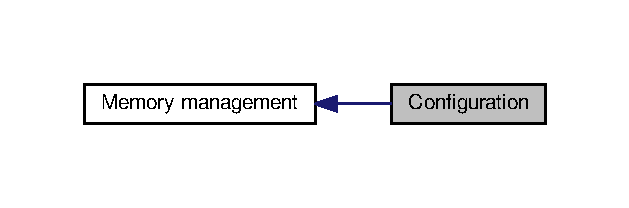
\includegraphics[width=302pt]{group__mem__cfg}
\end{center}
\end{figure}
\subsubsection*{e\-Solid memory allocator override}
\begin{DoxyCompactItemize}
\item 
\hypertarget{group__mem__cfg_ga543701ab60ff8b87e4e1ec9ea0b03491}{\#define {\bfseries O\-P\-T\-\_\-\-M\-E\-M\-\_\-\-A\-L\-L\-O\-C}~malloc}\label{group__mem__cfg_ga543701ab60ff8b87e4e1ec9ea0b03491}

\item 
\hypertarget{group__mem__cfg_gaab59d354bf34173761c3f95d0662c22e}{\#define {\bfseries O\-P\-T\-\_\-\-M\-E\-M\-\_\-\-F\-R\-E\-E}~free}\label{group__mem__cfg_gaab59d354bf34173761c3f95d0662c22e}

\end{DoxyCompactItemize}


\subsubsection{Detailed Description}

\section{Data Structure Documentation}
\hypertarget{structesDMemHandle}{\subsection{es\-D\-Mem\-Handle Struct Reference}
\label{structesDMemHandle}\index{es\-D\-Mem\-Handle@{es\-D\-Mem\-Handle}}
}


Dynamic memory instance handle structure.  




{\ttfamily \#include $<$mem.\-h$>$}



Collaboration diagram for es\-D\-Mem\-Handle\-:\nopagebreak
\begin{figure}[H]
\begin{center}
\leavevmode
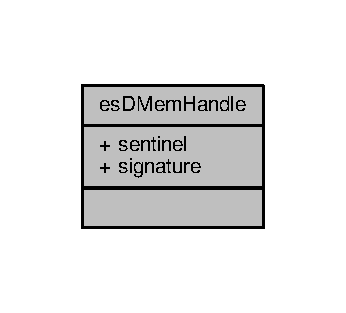
\includegraphics[width=166pt]{structesDMemHandle__coll__graph}
\end{center}
\end{figure}
\subsubsection*{Data Fields}
\begin{DoxyCompactItemize}
\item 
struct d\-Mem\-Block $\ast$ \hyperlink{structesDMemHandle_a64c2d859ebf90e27873f20e1cbbc3bb8}{sentinel}
\begin{DoxyCompactList}\small\item\em Pointer to the memory sentinel. \end{DoxyCompactList}\item 
port\-Reg\-\_\-\-T \hyperlink{structesDMemHandle_a471b42b8a335144bbb79ab89c0c3d170}{signature}
\begin{DoxyCompactList}\small\item\em Structure signature, used during development only. \end{DoxyCompactList}\end{DoxyCompactItemize}


\subsubsection{Detailed Description}
Dynamic memory instance handle structure. 

This structure holds information about dynamic memory instance. \begin{DoxySeeAlso}{See Also}
\hyperlink{group__mem__intf_ga10ef80121c0c742b9ad81f24eff91c7f}{es\-D\-Mem\-Init()} 
\end{DoxySeeAlso}
\begin{DoxyParagraph}{Object class\-:}
Regular {\bfseries A\-P\-I} object, this object is part of the application programming interface. 
\end{DoxyParagraph}
\begin{Desc}
\item[Examples\-: ]\par
\hyperlink{dmem_init1_8c-example}{dmem\-\_\-init1.\-c}, \hyperlink{dmem_init2_8c-example}{dmem\-\_\-init2.\-c}, and \hyperlink{dmem_two_buffs_8c-example}{dmem\-\_\-two\-\_\-buffs.\-c}.\end{Desc}


\subsubsection{Field Documentation}
\hypertarget{structesDMemHandle_a64c2d859ebf90e27873f20e1cbbc3bb8}{\index{es\-D\-Mem\-Handle@{es\-D\-Mem\-Handle}!sentinel@{sentinel}}
\index{sentinel@{sentinel}!esDMemHandle@{es\-D\-Mem\-Handle}}
\paragraph[{sentinel}]{\setlength{\rightskip}{0pt plus 5cm}struct d\-Mem\-Block$\ast$ es\-D\-Mem\-Handle\-::sentinel}}\label{structesDMemHandle_a64c2d859ebf90e27873f20e1cbbc3bb8}


Pointer to the memory sentinel. 

\hypertarget{structesDMemHandle_a471b42b8a335144bbb79ab89c0c3d170}{\index{es\-D\-Mem\-Handle@{es\-D\-Mem\-Handle}!signature@{signature}}
\index{signature@{signature}!esDMemHandle@{es\-D\-Mem\-Handle}}
\paragraph[{signature}]{\setlength{\rightskip}{0pt plus 5cm}port\-Reg\-\_\-\-T es\-D\-Mem\-Handle\-::signature}}\label{structesDMemHandle_a471b42b8a335144bbb79ab89c0c3d170}


Structure signature, used during development only. 



The documentation for this struct was generated from the following file\-:\begin{DoxyCompactItemize}
\item 
\hyperlink{mem_8h}{mem.\-h}\end{DoxyCompactItemize}

\hypertarget{structesMemStatus}{\subsection{es\-Mem\-Status Struct Reference}
\label{structesMemStatus}\index{es\-Mem\-Status@{es\-Mem\-Status}}
}


Memory status structure.  




{\ttfamily \#include $<$mem.\-h$>$}



Collaboration diagram for es\-Mem\-Status\-:\nopagebreak
\begin{figure}[H]
\begin{center}
\leavevmode
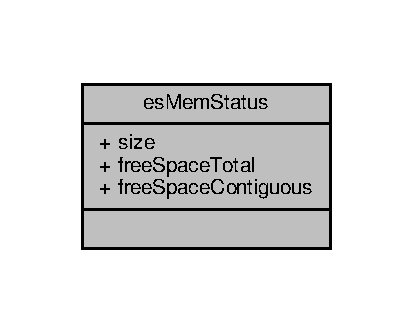
\includegraphics[width=198pt]{structesMemStatus__coll__graph}
\end{center}
\end{figure}
\subsubsection*{Data Fields}
\begin{DoxyCompactItemize}
\item 
size\-\_\-t \hyperlink{structesMemStatus_a380e3d7b616ea3b5b2116c643616f170}{size}
\begin{DoxyCompactList}\small\item\em Size of dynamic memory. \end{DoxyCompactList}\item 
size\-\_\-t \hyperlink{structesMemStatus_a7e03e413141601c2486fd55e8d4c6daf}{free\-Space\-Total}
\begin{DoxyCompactList}\small\item\em Total free space. \end{DoxyCompactList}\item 
size\-\_\-t \hyperlink{structesMemStatus_ab9abe5784bc4bb701ee759a2e02bfd8d}{free\-Space\-Contiguous}
\begin{DoxyCompactList}\small\item\em Contiguous free space. \end{DoxyCompactList}\end{DoxyCompactItemize}


\subsubsection{Detailed Description}
Memory status structure. 

This structure is used to get the status of a memory instance. Memory instance can be of type {\ttfamily static}, {\ttfamily dynamic} and {\ttfamily pool}. \begin{DoxySeeAlso}{See Also}
\hyperlink{group__mem__intf_ga87b817ce71357521c4cd43a9cb587201}{es\-S\-Mem\-Update\-Status\-I()}, \hyperlink{group__mem__intf_gab568f5b51f11f2bc315412c35bfc28e9}{es\-P\-Mem\-Update\-Status\-I()}, \hyperlink{group__mem__intf_gad1bddd779876d000f8906ec7ac747fa4}{es\-D\-Mem\-Update\-Status\-I()} 
\end{DoxySeeAlso}
\begin{DoxyParagraph}{Object class\-:}
Regular {\bfseries A\-P\-I} object, this object is part of the application programming interface. 
\end{DoxyParagraph}


\subsubsection{Field Documentation}
\hypertarget{structesMemStatus_a380e3d7b616ea3b5b2116c643616f170}{\index{es\-Mem\-Status@{es\-Mem\-Status}!size@{size}}
\index{size@{size}!esMemStatus@{es\-Mem\-Status}}
\paragraph[{size}]{\setlength{\rightskip}{0pt plus 5cm}size\-\_\-t es\-Mem\-Status\-::size}}\label{structesMemStatus_a380e3d7b616ea3b5b2116c643616f170}


Size of dynamic memory. 

\hypertarget{structesMemStatus_a7e03e413141601c2486fd55e8d4c6daf}{\index{es\-Mem\-Status@{es\-Mem\-Status}!free\-Space\-Total@{free\-Space\-Total}}
\index{free\-Space\-Total@{free\-Space\-Total}!esMemStatus@{es\-Mem\-Status}}
\paragraph[{free\-Space\-Total}]{\setlength{\rightskip}{0pt plus 5cm}size\-\_\-t es\-Mem\-Status\-::free\-Space\-Total}}\label{structesMemStatus_a7e03e413141601c2486fd55e8d4c6daf}


Total free space. 

\hypertarget{structesMemStatus_ab9abe5784bc4bb701ee759a2e02bfd8d}{\index{es\-Mem\-Status@{es\-Mem\-Status}!free\-Space\-Contiguous@{free\-Space\-Contiguous}}
\index{free\-Space\-Contiguous@{free\-Space\-Contiguous}!esMemStatus@{es\-Mem\-Status}}
\paragraph[{free\-Space\-Contiguous}]{\setlength{\rightskip}{0pt plus 5cm}size\-\_\-t es\-Mem\-Status\-::free\-Space\-Contiguous}}\label{structesMemStatus_ab9abe5784bc4bb701ee759a2e02bfd8d}


Contiguous free space. 



The documentation for this struct was generated from the following file\-:\begin{DoxyCompactItemize}
\item 
\hyperlink{mem_8h}{mem.\-h}\end{DoxyCompactItemize}

\hypertarget{structesPMemHandle}{\subsection{es\-P\-Mem\-Handle Struct Reference}
\label{structesPMemHandle}\index{es\-P\-Mem\-Handle@{es\-P\-Mem\-Handle}}
}


Pool memory instance handle structure.  




{\ttfamily \#include $<$mem.\-h$>$}



Collaboration diagram for es\-P\-Mem\-Handle\-:\nopagebreak
\begin{figure}[H]
\begin{center}
\leavevmode
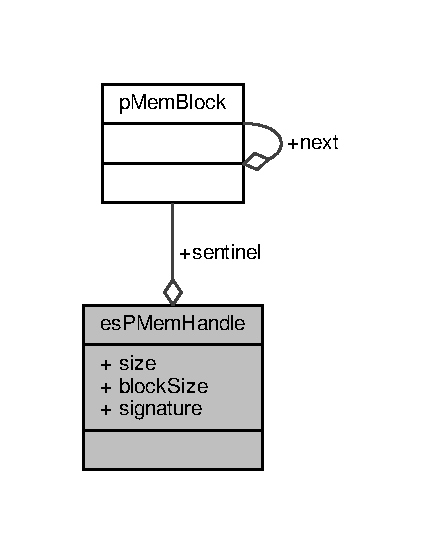
\includegraphics[width=203pt]{structesPMemHandle__coll__graph}
\end{center}
\end{figure}
\subsubsection*{Data Fields}
\begin{DoxyCompactItemize}
\item 
struct \hyperlink{structpMemBlock}{p\-Mem\-Block} $\ast$ \hyperlink{structesPMemHandle_a95b980208def4ca8c17c343aed282cd7}{sentinel}
\begin{DoxyCompactList}\small\item\em Pointer to the pool sentinel. \end{DoxyCompactList}\item 
size\-\_\-t \hyperlink{structesPMemHandle_a2ef5d8986c5e117c8ab5214e89ea021b}{size}
\begin{DoxyCompactList}\small\item\em The size of pool memory. \end{DoxyCompactList}\item 
size\-\_\-t \hyperlink{structesPMemHandle_a4498b86739feeabac46a7c2f457b3909}{block\-Size}
\begin{DoxyCompactList}\small\item\em Size of one block. \end{DoxyCompactList}\item 
port\-Reg\-\_\-\-T \hyperlink{structesPMemHandle_a16a84810e44eeed16fb9475f2f07001f}{signature}
\begin{DoxyCompactList}\small\item\em Structure signature, used during development only. \end{DoxyCompactList}\end{DoxyCompactItemize}


\subsubsection{Detailed Description}
Pool memory instance handle structure. 

This structure holds information about pool memory instance. {\ttfamily This} structure hold information about pool and block sizes. Additionally, it holds a guard member which will ensure mutual exclusion in preemption environments. \begin{DoxySeeAlso}{See Also}
\hyperlink{group__mem__intf_gac151cf4385488838b0507936e67e2584}{es\-P\-Mem\-Init()} 
\end{DoxySeeAlso}
\begin{DoxyParagraph}{Object class\-:}
Regular {\bfseries A\-P\-I} object, this object is part of the application programming interface. 
\end{DoxyParagraph}
\begin{Desc}
\item[Examples\-: ]\par
\hyperlink{dmem_init2_8c-example}{dmem\-\_\-init2.\-c}, \hyperlink{dmem_two_buffs_8c-example}{dmem\-\_\-two\-\_\-buffs.\-c}, \hyperlink{pmem_init1_8c-example}{pmem\-\_\-init1.\-c}, \hyperlink{pmem_init2_8c-example}{pmem\-\_\-init2.\-c}, \hyperlink{pmem_init3_8c-example}{pmem\-\_\-init3.\-c}, and \hyperlink{pmem_two_buffs_8c-example}{pmem\-\_\-two\-\_\-buffs.\-c}.\end{Desc}


\subsubsection{Field Documentation}
\hypertarget{structesPMemHandle_a95b980208def4ca8c17c343aed282cd7}{\index{es\-P\-Mem\-Handle@{es\-P\-Mem\-Handle}!sentinel@{sentinel}}
\index{sentinel@{sentinel}!esPMemHandle@{es\-P\-Mem\-Handle}}
\paragraph[{sentinel}]{\setlength{\rightskip}{0pt plus 5cm}struct {\bf p\-Mem\-Block}$\ast$ es\-P\-Mem\-Handle\-::sentinel}}\label{structesPMemHandle_a95b980208def4ca8c17c343aed282cd7}


Pointer to the pool sentinel. 

\hypertarget{structesPMemHandle_a2ef5d8986c5e117c8ab5214e89ea021b}{\index{es\-P\-Mem\-Handle@{es\-P\-Mem\-Handle}!size@{size}}
\index{size@{size}!esPMemHandle@{es\-P\-Mem\-Handle}}
\paragraph[{size}]{\setlength{\rightskip}{0pt plus 5cm}size\-\_\-t es\-P\-Mem\-Handle\-::size}}\label{structesPMemHandle_a2ef5d8986c5e117c8ab5214e89ea021b}


The size of pool memory. 

\hypertarget{structesPMemHandle_a4498b86739feeabac46a7c2f457b3909}{\index{es\-P\-Mem\-Handle@{es\-P\-Mem\-Handle}!block\-Size@{block\-Size}}
\index{block\-Size@{block\-Size}!esPMemHandle@{es\-P\-Mem\-Handle}}
\paragraph[{block\-Size}]{\setlength{\rightskip}{0pt plus 5cm}size\-\_\-t es\-P\-Mem\-Handle\-::block\-Size}}\label{structesPMemHandle_a4498b86739feeabac46a7c2f457b3909}


Size of one block. 

\hypertarget{structesPMemHandle_a16a84810e44eeed16fb9475f2f07001f}{\index{es\-P\-Mem\-Handle@{es\-P\-Mem\-Handle}!signature@{signature}}
\index{signature@{signature}!esPMemHandle@{es\-P\-Mem\-Handle}}
\paragraph[{signature}]{\setlength{\rightskip}{0pt plus 5cm}port\-Reg\-\_\-\-T es\-P\-Mem\-Handle\-::signature}}\label{structesPMemHandle_a16a84810e44eeed16fb9475f2f07001f}


Structure signature, used during development only. 



The documentation for this struct was generated from the following file\-:\begin{DoxyCompactItemize}
\item 
\hyperlink{mem_8h}{mem.\-h}\end{DoxyCompactItemize}

\hypertarget{structesSMemHandle}{\subsection{es\-S\-Mem\-Handle Struct Reference}
\label{structesSMemHandle}\index{es\-S\-Mem\-Handle@{es\-S\-Mem\-Handle}}
}


Static memory instance handle structure.  




{\ttfamily \#include $<$mem.\-h$>$}



Collaboration diagram for es\-S\-Mem\-Handle\-:\nopagebreak
\begin{figure}[H]
\begin{center}
\leavevmode
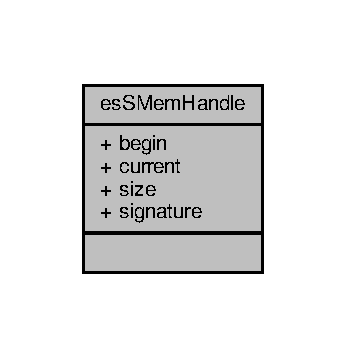
\includegraphics[width=166pt]{structesSMemHandle__coll__graph}
\end{center}
\end{figure}
\subsubsection*{Data Fields}
\begin{DoxyCompactItemize}
\item 
port\-Reg\-\_\-\-T $\ast$ \hyperlink{structesSMemHandle_a01da81c99962c4e30bc5286a95e1c912}{begin}
\begin{DoxyCompactList}\small\item\em Pointer to the beginning of static memory. \end{DoxyCompactList}\item 
port\-Reg\-\_\-\-T \hyperlink{structesSMemHandle_a2ffccb4ce219c893b0de4bb277a4103d}{current}
\begin{DoxyCompactList}\small\item\em Current index of managed memory. \end{DoxyCompactList}\item 
size\-\_\-t \hyperlink{structesSMemHandle_a9f70491a315a88d0e01edc29e87da9b0}{size}
\begin{DoxyCompactList}\small\item\em The size of static memory. \end{DoxyCompactList}\item 
port\-Reg\-\_\-\-T \hyperlink{structesSMemHandle_a026a8283657eb726a0c9c559e455153a}{signature}
\begin{DoxyCompactList}\small\item\em Structure signature, used during development only. \end{DoxyCompactList}\end{DoxyCompactItemize}


\subsubsection{Detailed Description}
Static memory instance handle structure. 

This structure holds information about static memory instance. \begin{DoxyParagraph}{Object class\-:}
Regular {\bfseries A\-P\-I} object, this object is part of the application programming interface. 
\end{DoxyParagraph}


\subsubsection{Field Documentation}
\hypertarget{structesSMemHandle_a01da81c99962c4e30bc5286a95e1c912}{\index{es\-S\-Mem\-Handle@{es\-S\-Mem\-Handle}!begin@{begin}}
\index{begin@{begin}!esSMemHandle@{es\-S\-Mem\-Handle}}
\paragraph[{begin}]{\setlength{\rightskip}{0pt plus 5cm}port\-Reg\-\_\-\-T$\ast$ es\-S\-Mem\-Handle\-::begin}}\label{structesSMemHandle_a01da81c99962c4e30bc5286a95e1c912}


Pointer to the beginning of static memory. 

\hypertarget{structesSMemHandle_a2ffccb4ce219c893b0de4bb277a4103d}{\index{es\-S\-Mem\-Handle@{es\-S\-Mem\-Handle}!current@{current}}
\index{current@{current}!esSMemHandle@{es\-S\-Mem\-Handle}}
\paragraph[{current}]{\setlength{\rightskip}{0pt plus 5cm}port\-Reg\-\_\-\-T es\-S\-Mem\-Handle\-::current}}\label{structesSMemHandle_a2ffccb4ce219c893b0de4bb277a4103d}


Current index of managed memory. 

\hypertarget{structesSMemHandle_a9f70491a315a88d0e01edc29e87da9b0}{\index{es\-S\-Mem\-Handle@{es\-S\-Mem\-Handle}!size@{size}}
\index{size@{size}!esSMemHandle@{es\-S\-Mem\-Handle}}
\paragraph[{size}]{\setlength{\rightskip}{0pt plus 5cm}size\-\_\-t es\-S\-Mem\-Handle\-::size}}\label{structesSMemHandle_a9f70491a315a88d0e01edc29e87da9b0}


The size of static memory. 

\hypertarget{structesSMemHandle_a026a8283657eb726a0c9c559e455153a}{\index{es\-S\-Mem\-Handle@{es\-S\-Mem\-Handle}!signature@{signature}}
\index{signature@{signature}!esSMemHandle@{es\-S\-Mem\-Handle}}
\paragraph[{signature}]{\setlength{\rightskip}{0pt plus 5cm}port\-Reg\-\_\-\-T es\-S\-Mem\-Handle\-::signature}}\label{structesSMemHandle_a026a8283657eb726a0c9c559e455153a}


Structure signature, used during development only. 



The documentation for this struct was generated from the following file\-:\begin{DoxyCompactItemize}
\item 
\hyperlink{mem_8h}{mem.\-h}\end{DoxyCompactItemize}

\hypertarget{structpMemBlock}{\subsection{p\-Mem\-Block Struct Reference}
\label{structpMemBlock}\index{p\-Mem\-Block@{p\-Mem\-Block}}
}


Pool allocator header structure.  




Collaboration diagram for p\-Mem\-Block\-:\nopagebreak
\begin{figure}[H]
\begin{center}
\leavevmode
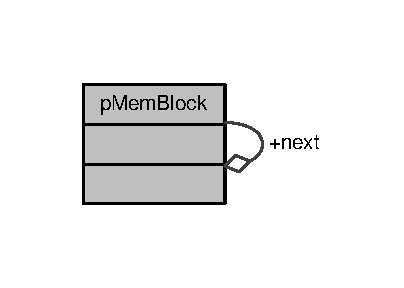
\includegraphics[width=194pt]{structpMemBlock__coll__graph}
\end{center}
\end{figure}
\subsubsection*{Data Fields}
\begin{DoxyCompactItemize}
\item 
struct \hyperlink{structpMemBlock}{p\-Mem\-Block} $\ast$ \hyperlink{structpMemBlock_af04fa2bbd0fd3da6baf2ac08ce54455e}{next}
\begin{DoxyCompactList}\small\item\em Next free block. \end{DoxyCompactList}\end{DoxyCompactItemize}


\subsubsection{Detailed Description}
Pool allocator header structure. 

\subsubsection{Field Documentation}
\hypertarget{structpMemBlock_af04fa2bbd0fd3da6baf2ac08ce54455e}{\index{p\-Mem\-Block@{p\-Mem\-Block}!next@{next}}
\index{next@{next}!pMemBlock@{p\-Mem\-Block}}
\paragraph[{next}]{\setlength{\rightskip}{0pt plus 5cm}struct {\bf p\-Mem\-Block}$\ast$ p\-Mem\-Block\-::next}}\label{structpMemBlock_af04fa2bbd0fd3da6baf2ac08ce54455e}


Next free block. 



The documentation for this struct was generated from the following file\-:\begin{DoxyCompactItemize}
\item 
\hyperlink{mem_8c}{mem.\-c}\end{DoxyCompactItemize}

\section{File Documentation}
\hypertarget{mem_8c}{\subsection{mem.\-c File Reference}
\label{mem_8c}\index{mem.\-c@{mem.\-c}}
}


Memory Management Implementation.  


{\ttfamily \#include \char`\"{}kernel/lock.\-h\char`\"{}}\\*
{\ttfamily \#include \char`\"{}kernel/bitop.\-h\char`\"{}}\\*
{\ttfamily \#include \char`\"{}mem/mem.\-h\char`\"{}}\\*
{\ttfamily \#include \char`\"{}arch/cpu.\-h\char`\"{}}\\*
Include dependency graph for mem.\-c\-:\nopagebreak
\begin{figure}[H]
\begin{center}
\leavevmode
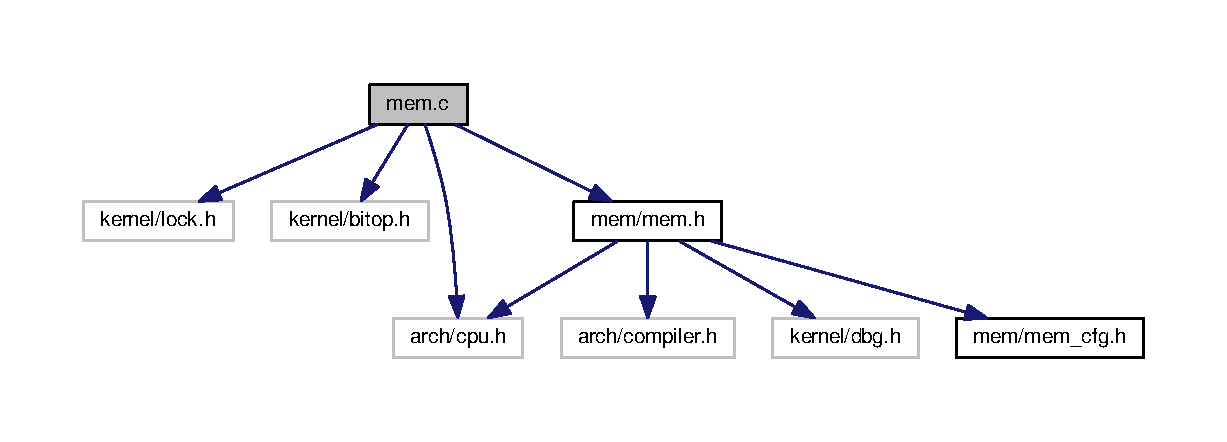
\includegraphics[width=350pt]{mem_8c__incl}
\end{center}
\end{figure}
\subsubsection*{Data Structures}
\begin{DoxyCompactItemize}
\item 
struct \hyperlink{structpMemBlock}{p\-Mem\-Block}
\begin{DoxyCompactList}\small\item\em Pool allocator header structure. \end{DoxyCompactList}\end{DoxyCompactItemize}
\subsubsection*{Macros}
\begin{DoxyCompactItemize}
\item 
\#define \hyperlink{group__mem__impl_gae0fa2c7ba98034d2b0a59299edc64c66}{S\-M\-E\-M\-\_\-\-S\-I\-G\-N\-A\-T\-U\-R\-E}~((port\-Reg\-\_\-\-T)0x\-D\-E\-A\-D\-B\-E\-E\-D\-U)
\begin{DoxyCompactList}\small\item\em Signature for static memory manager. \end{DoxyCompactList}\item 
\#define \hyperlink{group__mem__impl_ga37e53ccf6c132baa9a610318a18c312e}{P\-M\-E\-M\-\_\-\-S\-I\-G\-N\-A\-T\-U\-R\-E}~((port\-Reg\-\_\-\-T)0x\-D\-E\-A\-D\-B\-E\-E\-E\-U)
\begin{DoxyCompactList}\small\item\em Signature for pool memory manager. \end{DoxyCompactList}\item 
\#define \hyperlink{group__mem__impl_ga6aeb51ed48814f4d3e0c8bd5640d4533}{D\-M\-E\-M\-\_\-\-S\-I\-G\-N\-A\-T\-U\-R\-E}~((port\-Reg\-\_\-\-T)0x\-D\-E\-A\-D\-B\-E\-E\-F\-U)
\begin{DoxyCompactList}\small\item\em Signature for dynamic memory manager. \end{DoxyCompactList}\end{DoxyCompactItemize}
\subsubsection*{Typedefs}
\begin{DoxyCompactItemize}
\item 
typedef struct d\-Mem\-Block \hyperlink{group__mem__impl_ga426d7b4525653e3c90bf3fef9d443373}{d\-Mem\-Block\-\_\-\-T}
\begin{DoxyCompactList}\small\item\em Dynamic allocator memory block header type. \end{DoxyCompactList}\item 
typedef struct \hyperlink{structpMemBlock}{p\-Mem\-Block} \hyperlink{group__mem__impl_gad80b53ee7c1b89f2d48d9670b0c09ceb}{p\-Mem\-Block\-\_\-\-T}
\begin{DoxyCompactList}\small\item\em Pool allocator header type. \end{DoxyCompactList}\end{DoxyCompactItemize}
\subsubsection*{Functions}
\begin{DoxyCompactItemize}
\item 
struct \hyperlink{group__mem__impl_ga4314f62895ea8335b19545c0f6a74e34}{P\-O\-R\-T\-\_\-\-C\-\_\-\-A\-L\-I\-G\-N} (P\-O\-R\-T\-\_\-\-D\-E\-F\-\_\-\-D\-A\-T\-A\-\_\-\-A\-L\-I\-G\-N\-M\-E\-N\-T)
\begin{DoxyCompactList}\small\item\em Dynamic allocator memory block header structure. \end{DoxyCompactList}\item 
\hyperlink{group__mem__impl_gade934104528d9fb269eb5aef4041daca}{D\-E\-C\-L\-\_\-\-M\-O\-D\-U\-L\-E\-\_\-\-I\-N\-F\-O} (\char`\"{}M\-E\-M\char`\"{},\char`\"{}Memory management\char`\"{},\char`\"{}Nenad Radulovic\char`\"{})
\begin{DoxyCompactList}\small\item\em Module information. \end{DoxyCompactList}\item 
void \hyperlink{group__mem__impl_ga53acef4ba27e5e401ac2e1f862e07a8b}{es\-S\-Mem\-Init} (\hyperlink{group__mem__intf_gabf19a317cc22713cfb45ae1e43d34d7e}{es\-S\-Mem\-Handle\-\_\-\-T} $\ast$handle, void $\ast$storage, size\-\_\-t storage\-Size)
\begin{DoxyCompactList}\small\item\em Initializes static memory instance. \end{DoxyCompactList}\item 
void $\ast$ \hyperlink{group__mem__impl_ga2e2086778aa0eb21156044730a1f380b}{es\-S\-Mem\-Alloc\-I} (\hyperlink{group__mem__intf_gabf19a317cc22713cfb45ae1e43d34d7e}{es\-S\-Mem\-Handle\-\_\-\-T} $\ast$handle, size\-\_\-t size)
\begin{DoxyCompactList}\small\item\em Allocates static memory of size {\ttfamily size}. \end{DoxyCompactList}\item 
void $\ast$ \hyperlink{group__mem__impl_ga23c0a40e0c40dabed8c22d9d65709c65}{es\-S\-Mem\-Alloc} (\hyperlink{group__mem__intf_gabf19a317cc22713cfb45ae1e43d34d7e}{es\-S\-Mem\-Handle\-\_\-\-T} $\ast$handle, size\-\_\-t size)
\begin{DoxyCompactList}\small\item\em Allocates static memory of size {\ttfamily size}. \end{DoxyCompactList}\item 
void \hyperlink{group__mem__impl_ga87b817ce71357521c4cd43a9cb587201}{es\-S\-Mem\-Update\-Status\-I} (\hyperlink{group__mem__intf_gabf19a317cc22713cfb45ae1e43d34d7e}{es\-S\-Mem\-Handle\-\_\-\-T} $\ast$handle, \hyperlink{group__mem__intf_ga0eb568b68247d93e2db804a681de0e9e}{es\-Mem\-Status\-\_\-\-T} $\ast$status)
\begin{DoxyCompactList}\small\item\em Returns various information about given memory instance. \end{DoxyCompactList}\item 
void \hyperlink{group__mem__impl_gac0ad18ef5c9332358a4d0a5ded270f34}{es\-S\-Mem\-Update\-Status} (\hyperlink{group__mem__intf_gabf19a317cc22713cfb45ae1e43d34d7e}{es\-S\-Mem\-Handle\-\_\-\-T} $\ast$handle, \hyperlink{group__mem__intf_ga0eb568b68247d93e2db804a681de0e9e}{es\-Mem\-Status\-\_\-\-T} $\ast$status)
\begin{DoxyCompactList}\small\item\em Returns various information about given memory instance. \end{DoxyCompactList}\item 
void \hyperlink{group__mem__impl_ga0cf65ff195adf771ccc1fa12d61dc74a}{es\-P\-Mem\-Init} (\hyperlink{group__mem__intf_gaf82f01d26c4f6bc9a2b672a673b09ce2}{es\-P\-Mem\-Handle\-\_\-\-T} $\ast$handle, void $\ast$array, size\-\_\-t array\-Size, size\-\_\-t block\-Size)
\begin{DoxyCompactList}\small\item\em Initializes pool memory instance. \end{DoxyCompactList}\item 
size\-\_\-t \hyperlink{group__mem__impl_gab82743b6c82847c748bf5193f0f211ec}{es\-P\-Mem\-Calc\-Pool\-Size} (size\-\_\-t blocks, size\-\_\-t block\-Size)
\begin{DoxyCompactList}\small\item\em Calculates required reserved memory size for defined number of blocks. \end{DoxyCompactList}\item 
void $\ast$ \hyperlink{group__mem__impl_gabdacce602565fcd6a186c2834cb74488}{es\-P\-Mem\-Alloc\-I} (\hyperlink{group__mem__intf_gaf82f01d26c4f6bc9a2b672a673b09ce2}{es\-P\-Mem\-Handle\-\_\-\-T} $\ast$handle)
\begin{DoxyCompactList}\small\item\em Allocate one block from memory pool. \end{DoxyCompactList}\item 
void $\ast$ \hyperlink{group__mem__impl_gac750c9ec7780f5dc616e8a04a6668f34}{es\-P\-Mem\-Alloc} (\hyperlink{group__mem__intf_gaf82f01d26c4f6bc9a2b672a673b09ce2}{es\-P\-Mem\-Handle\-\_\-\-T} $\ast$handle)
\begin{DoxyCompactList}\small\item\em Allocate one block from memory pool. \end{DoxyCompactList}\item 
void \hyperlink{group__mem__impl_ga2c0f1b135c5639809b17dfe44e06f1b5}{es\-P\-Mem\-De\-Alloc\-I} (\hyperlink{group__mem__intf_gaf82f01d26c4f6bc9a2b672a673b09ce2}{es\-P\-Mem\-Handle\-\_\-\-T} $\ast$handle, void $\ast$mem)
\begin{DoxyCompactList}\small\item\em Oslobadja prethodno alocirani blok. \end{DoxyCompactList}\item 
void \hyperlink{group__mem__impl_gacd393e705fe5531cae380cc9b68f7a23}{es\-P\-Mem\-De\-Alloc} (\hyperlink{group__mem__intf_gaf82f01d26c4f6bc9a2b672a673b09ce2}{es\-P\-Mem\-Handle\-\_\-\-T} $\ast$handle, void $\ast$mem)
\begin{DoxyCompactList}\small\item\em Oslobadja prethodno alocirani blok. \end{DoxyCompactList}\item 
void \hyperlink{group__mem__impl_gab568f5b51f11f2bc315412c35bfc28e9}{es\-P\-Mem\-Update\-Status\-I} (\hyperlink{group__mem__intf_gaf82f01d26c4f6bc9a2b672a673b09ce2}{es\-P\-Mem\-Handle\-\_\-\-T} $\ast$handle, \hyperlink{group__mem__intf_ga0eb568b68247d93e2db804a681de0e9e}{es\-Mem\-Status\-\_\-\-T} $\ast$status)
\begin{DoxyCompactList}\small\item\em Vraca statusne informacije pool memorije. \end{DoxyCompactList}\item 
void \hyperlink{group__mem__impl_ga8148d4ad98ed5e9ecc04b7983433555e}{es\-P\-Mem\-Update\-Status} (\hyperlink{group__mem__intf_gaf82f01d26c4f6bc9a2b672a673b09ce2}{es\-P\-Mem\-Handle\-\_\-\-T} $\ast$handle, \hyperlink{group__mem__intf_ga0eb568b68247d93e2db804a681de0e9e}{es\-Mem\-Status\-\_\-\-T} $\ast$status)
\begin{DoxyCompactList}\small\item\em Vraca statusne informacije pool memorije. \end{DoxyCompactList}\item 
void \hyperlink{group__mem__impl_ga10ef80121c0c742b9ad81f24eff91c7f}{es\-D\-Mem\-Init} (\hyperlink{group__mem__intf_gacaaf771b18b3da8fa3b67a466390080e}{es\-D\-Mem\-Handle\-\_\-\-T} $\ast$handle, void $\ast$storage, size\-\_\-t storage\-Size)
\begin{DoxyCompactList}\small\item\em Inicijalizuje dinamican memorijski alokator. \end{DoxyCompactList}\item 
void $\ast$ \hyperlink{group__mem__impl_ga807a7d2e705b1802b7671c0c903611a6}{es\-D\-Mem\-Alloc\-I} (\hyperlink{group__mem__intf_gacaaf771b18b3da8fa3b67a466390080e}{es\-D\-Mem\-Handle\-\_\-\-T} $\ast$handle, size\-\_\-t size)
\begin{DoxyCompactList}\small\item\em Dodeljuje memorijski prostor velicine {\ttfamily size}. \end{DoxyCompactList}\item 
void $\ast$ \hyperlink{group__mem__impl_ga7aa5c1f6bda178e4860f0727b1fd3590}{es\-D\-Mem\-Alloc} (\hyperlink{group__mem__intf_gacaaf771b18b3da8fa3b67a466390080e}{es\-D\-Mem\-Handle\-\_\-\-T} $\ast$handle, size\-\_\-t size)
\begin{DoxyCompactList}\small\item\em Dodeljuje memorijski prostor velicine {\ttfamily size}. \end{DoxyCompactList}\item 
void \hyperlink{group__mem__impl_gad56192526f2b6ec1f927d21b15e1bc11}{es\-D\-Mem\-De\-Alloc\-I} (\hyperlink{group__mem__intf_gacaaf771b18b3da8fa3b67a466390080e}{es\-D\-Mem\-Handle\-\_\-\-T} $\ast$handle, void $\ast$mem)
\begin{DoxyCompactList}\small\item\em Reciklira memorijski prostor na koji pokazije {\ttfamily mem} pokazivac. \end{DoxyCompactList}\item 
void \hyperlink{group__mem__impl_gad63c5b88aae0a4626763d934fdcdc9d1}{es\-D\-Mem\-De\-Alloc} (\hyperlink{group__mem__intf_gacaaf771b18b3da8fa3b67a466390080e}{es\-D\-Mem\-Handle\-\_\-\-T} $\ast$handle, void $\ast$mem)
\begin{DoxyCompactList}\small\item\em Reciklira memorijski prostor na koji pokazije {\ttfamily mem} pokazivac. \end{DoxyCompactList}\item 
void \hyperlink{group__mem__impl_gad1bddd779876d000f8906ec7ac747fa4}{es\-D\-Mem\-Update\-Status\-I} (\hyperlink{group__mem__intf_gacaaf771b18b3da8fa3b67a466390080e}{es\-D\-Mem\-Handle\-\_\-\-T} $\ast$handle, \hyperlink{group__mem__intf_ga0eb568b68247d93e2db804a681de0e9e}{es\-Mem\-Status\-\_\-\-T} $\ast$status)
\begin{DoxyCompactList}\small\item\em Vraca velicinu trenutno slobodne memorije u bajtovima. \end{DoxyCompactList}\item 
void \hyperlink{group__mem__impl_ga22ab58d97d2519dccf91220f029ac87f}{es\-D\-Mem\-Update\-Status} (\hyperlink{group__mem__intf_gacaaf771b18b3da8fa3b67a466390080e}{es\-D\-Mem\-Handle\-\_\-\-T} $\ast$handle, \hyperlink{group__mem__intf_ga0eb568b68247d93e2db804a681de0e9e}{es\-Mem\-Status\-\_\-\-T} $\ast$status)
\begin{DoxyCompactList}\small\item\em Vraca velicinu trenutno slobodne memorije u bajtovima. \end{DoxyCompactList}\end{DoxyCompactItemize}
\subsubsection*{Variables}
\begin{DoxyCompactItemize}
\item 
\hyperlink{group__mem__intf_gabf19a317cc22713cfb45ae1e43d34d7e}{es\-S\-Mem\-Handle\-\_\-\-T} \hyperlink{group__mem__impl_ga59214c7e13470c5e76c7b59c4f084b1c}{Def\-S\-Mem\-Handle}
\begin{DoxyCompactList}\small\item\em Default static memory handle. \end{DoxyCompactList}\item 
\hyperlink{group__mem__intf_gaf82f01d26c4f6bc9a2b672a673b09ce2}{es\-P\-Mem\-Handle\-\_\-\-T} \hyperlink{group__mem__impl_gafb0dc701e9679157a617a091843bcd7f}{Def\-P\-Mem\-Handle}
\begin{DoxyCompactList}\small\item\em Default pool memory handle. \end{DoxyCompactList}\item 
\hyperlink{group__mem__intf_gacaaf771b18b3da8fa3b67a466390080e}{es\-D\-Mem\-Handle\-\_\-\-T} \hyperlink{group__mem__impl_gae2d3f8ca3b99ba0a5b9d9518a7bc280b}{Def\-D\-Mem\-Handle}
\begin{DoxyCompactList}\small\item\em Default dynamic memory handle. \end{DoxyCompactList}\end{DoxyCompactItemize}


\subsubsection{Detailed Description}
Memory Management Implementation. \begin{DoxyAuthor}{Author}
Nenad Radulovic 
\end{DoxyAuthor}

\hypertarget{mem_8dox}{\subsection{mem.\-dox File Reference}
\label{mem_8dox}\index{mem.\-dox@{mem.\-dox}}
}

\hypertarget{mem_8h}{\subsection{mem.\-h File Reference}
\label{mem_8h}\index{mem.\-h@{mem.\-h}}
}


Memory Management A\-P\-I.  


{\ttfamily \#include \char`\"{}arch/compiler.\-h\char`\"{}}\\*
{\ttfamily \#include \char`\"{}arch/cpu.\-h\char`\"{}}\\*
{\ttfamily \#include \char`\"{}kernel/dbg.\-h\char`\"{}}\\*
{\ttfamily \#include \char`\"{}mem/mem\-\_\-cfg.\-h\char`\"{}}\\*
Include dependency graph for mem.\-h\-:\nopagebreak
\begin{figure}[H]
\begin{center}
\leavevmode
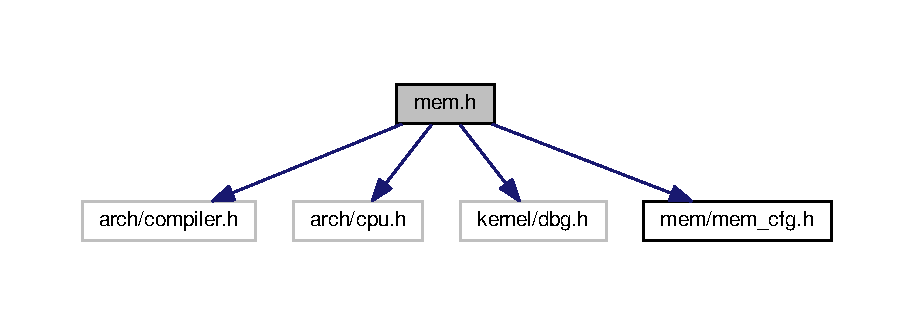
\includegraphics[width=350pt]{mem_8h__incl}
\end{center}
\end{figure}
This graph shows which files directly or indirectly include this file\-:\nopagebreak
\begin{figure}[H]
\begin{center}
\leavevmode
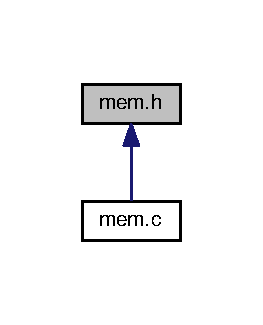
\includegraphics[width=126pt]{mem_8h__dep__incl}
\end{center}
\end{figure}
\subsubsection*{Data Structures}
\begin{DoxyCompactItemize}
\item 
struct \hyperlink{structesMemStatus}{es\-Mem\-Status}
\begin{DoxyCompactList}\small\item\em Memory status structure. \end{DoxyCompactList}\item 
struct \hyperlink{structesSMemHandle}{es\-S\-Mem\-Handle}
\begin{DoxyCompactList}\small\item\em Static memory instance handle structure. \end{DoxyCompactList}\item 
struct \hyperlink{structesPMemHandle}{es\-P\-Mem\-Handle}
\begin{DoxyCompactList}\small\item\em Pool memory instance handle structure. \end{DoxyCompactList}\item 
struct \hyperlink{structesDMemHandle}{es\-D\-Mem\-Handle}
\begin{DoxyCompactList}\small\item\em Dynamic memory instance handle structure. \end{DoxyCompactList}\end{DoxyCompactItemize}
\subsubsection*{Typedefs}
\begin{DoxyCompactItemize}
\item 
typedef struct \hyperlink{structesMemStatus}{es\-Mem\-Status} \hyperlink{group__mem__intf_ga0eb568b68247d93e2db804a681de0e9e}{es\-Mem\-Status\-\_\-\-T}
\begin{DoxyCompactList}\small\item\em Memory status type. \end{DoxyCompactList}\end{DoxyCompactItemize}
\begin{Indent}{\bf Static memory manager -\/ S\-Mem}\par
\begin{DoxyCompactItemize}
\item 
typedef struct \hyperlink{structesSMemHandle}{es\-S\-Mem\-Handle} \hyperlink{group__mem__intf_gabf19a317cc22713cfb45ae1e43d34d7e}{es\-S\-Mem\-Handle\-\_\-\-T}
\begin{DoxyCompactList}\small\item\em Static memory instance handle type. \end{DoxyCompactList}\end{DoxyCompactItemize}
\end{Indent}
\begin{Indent}{\bf Pool memory allocator -\/ P\-Mem}\par
\begin{DoxyCompactItemize}
\item 
typedef struct \hyperlink{structesPMemHandle}{es\-P\-Mem\-Handle} \hyperlink{group__mem__intf_gaf82f01d26c4f6bc9a2b672a673b09ce2}{es\-P\-Mem\-Handle\-\_\-\-T}
\begin{DoxyCompactList}\small\item\em Pool memory instance handle type. \end{DoxyCompactList}\end{DoxyCompactItemize}
\end{Indent}
\begin{Indent}{\bf Dynamic memory allocator -\/ D\-Mem}\par
\begin{DoxyCompactItemize}
\item 
typedef struct \hyperlink{structesDMemHandle}{es\-D\-Mem\-Handle} \hyperlink{group__mem__intf_gacaaf771b18b3da8fa3b67a466390080e}{es\-D\-Mem\-Handle\-\_\-\-T}
\begin{DoxyCompactList}\small\item\em Dynamic memory instance handle type. \end{DoxyCompactList}\end{DoxyCompactItemize}
\end{Indent}
\subsubsection*{Functions}
\begin{Indent}{\bf Static memory manager}\par
\begin{DoxyCompactItemize}
\item 
void \hyperlink{group__mem__intf_ga53acef4ba27e5e401ac2e1f862e07a8b}{es\-S\-Mem\-Init} (\hyperlink{group__mem__intf_gabf19a317cc22713cfb45ae1e43d34d7e}{es\-S\-Mem\-Handle\-\_\-\-T} $\ast$handle, void $\ast$storage, size\-\_\-t storage\-Size)
\begin{DoxyCompactList}\small\item\em Initializes static memory instance. \end{DoxyCompactList}\item 
void $\ast$ \hyperlink{group__mem__intf_ga2e2086778aa0eb21156044730a1f380b}{es\-S\-Mem\-Alloc\-I} (\hyperlink{group__mem__intf_gabf19a317cc22713cfb45ae1e43d34d7e}{es\-S\-Mem\-Handle\-\_\-\-T} $\ast$handle, size\-\_\-t size)
\begin{DoxyCompactList}\small\item\em Allocates static memory of size {\ttfamily size}. \end{DoxyCompactList}\item 
void $\ast$ \hyperlink{group__mem__intf_ga23c0a40e0c40dabed8c22d9d65709c65}{es\-S\-Mem\-Alloc} (\hyperlink{group__mem__intf_gabf19a317cc22713cfb45ae1e43d34d7e}{es\-S\-Mem\-Handle\-\_\-\-T} $\ast$handle, size\-\_\-t size)
\begin{DoxyCompactList}\small\item\em Allocates static memory of size {\ttfamily size}. \end{DoxyCompactList}\item 
void \hyperlink{group__mem__intf_ga87b817ce71357521c4cd43a9cb587201}{es\-S\-Mem\-Update\-Status\-I} (\hyperlink{group__mem__intf_gabf19a317cc22713cfb45ae1e43d34d7e}{es\-S\-Mem\-Handle\-\_\-\-T} $\ast$handle, \hyperlink{group__mem__intf_ga0eb568b68247d93e2db804a681de0e9e}{es\-Mem\-Status\-\_\-\-T} $\ast$status)
\begin{DoxyCompactList}\small\item\em Returns various information about given memory instance. \end{DoxyCompactList}\item 
void \hyperlink{group__mem__intf_gac0ad18ef5c9332358a4d0a5ded270f34}{es\-S\-Mem\-Update\-Status} (\hyperlink{group__mem__intf_gabf19a317cc22713cfb45ae1e43d34d7e}{es\-S\-Mem\-Handle\-\_\-\-T} $\ast$handle, \hyperlink{group__mem__intf_ga0eb568b68247d93e2db804a681de0e9e}{es\-Mem\-Status\-\_\-\-T} $\ast$status)
\begin{DoxyCompactList}\small\item\em Returns various information about given memory instance. \end{DoxyCompactList}\end{DoxyCompactItemize}
\end{Indent}
\begin{Indent}{\bf Pool memory manager}\par
\begin{DoxyCompactItemize}
\item 
void \hyperlink{group__mem__intf_gac151cf4385488838b0507936e67e2584}{es\-P\-Mem\-Init} (\hyperlink{group__mem__intf_gaf82f01d26c4f6bc9a2b672a673b09ce2}{es\-P\-Mem\-Handle\-\_\-\-T} $\ast$handle, void $\ast$pool, size\-\_\-t pool\-Size, size\-\_\-t block\-Size)
\begin{DoxyCompactList}\small\item\em Initializes pool memory instance. \end{DoxyCompactList}\item 
size\-\_\-t \hyperlink{group__mem__intf_gab82743b6c82847c748bf5193f0f211ec}{es\-P\-Mem\-Calc\-Pool\-Size} (size\-\_\-t blocks, size\-\_\-t block\-Size)
\begin{DoxyCompactList}\small\item\em Calculates required reserved memory size for defined number of blocks. \end{DoxyCompactList}\item 
void $\ast$ \hyperlink{group__mem__intf_gabdacce602565fcd6a186c2834cb74488}{es\-P\-Mem\-Alloc\-I} (\hyperlink{group__mem__intf_gaf82f01d26c4f6bc9a2b672a673b09ce2}{es\-P\-Mem\-Handle\-\_\-\-T} $\ast$handle)
\begin{DoxyCompactList}\small\item\em Allocate one block from memory pool. \end{DoxyCompactList}\item 
void $\ast$ \hyperlink{group__mem__intf_gac750c9ec7780f5dc616e8a04a6668f34}{es\-P\-Mem\-Alloc} (\hyperlink{group__mem__intf_gaf82f01d26c4f6bc9a2b672a673b09ce2}{es\-P\-Mem\-Handle\-\_\-\-T} $\ast$handle)
\begin{DoxyCompactList}\small\item\em Allocate one block from memory pool. \end{DoxyCompactList}\item 
void \hyperlink{group__mem__intf_ga2c0f1b135c5639809b17dfe44e06f1b5}{es\-P\-Mem\-De\-Alloc\-I} (\hyperlink{group__mem__intf_gaf82f01d26c4f6bc9a2b672a673b09ce2}{es\-P\-Mem\-Handle\-\_\-\-T} $\ast$handle, void $\ast$mem)
\begin{DoxyCompactList}\small\item\em Oslobadja prethodno alocirani blok. \end{DoxyCompactList}\item 
void \hyperlink{group__mem__intf_gacd393e705fe5531cae380cc9b68f7a23}{es\-P\-Mem\-De\-Alloc} (\hyperlink{group__mem__intf_gaf82f01d26c4f6bc9a2b672a673b09ce2}{es\-P\-Mem\-Handle\-\_\-\-T} $\ast$handle, void $\ast$mem)
\begin{DoxyCompactList}\small\item\em Oslobadja prethodno alocirani blok. \end{DoxyCompactList}\item 
void \hyperlink{group__mem__intf_gab568f5b51f11f2bc315412c35bfc28e9}{es\-P\-Mem\-Update\-Status\-I} (\hyperlink{group__mem__intf_gaf82f01d26c4f6bc9a2b672a673b09ce2}{es\-P\-Mem\-Handle\-\_\-\-T} $\ast$handle, \hyperlink{group__mem__intf_ga0eb568b68247d93e2db804a681de0e9e}{es\-Mem\-Status\-\_\-\-T} $\ast$status)
\begin{DoxyCompactList}\small\item\em Vraca statusne informacije pool memorije. \end{DoxyCompactList}\item 
void \hyperlink{group__mem__intf_ga8148d4ad98ed5e9ecc04b7983433555e}{es\-P\-Mem\-Update\-Status} (\hyperlink{group__mem__intf_gaf82f01d26c4f6bc9a2b672a673b09ce2}{es\-P\-Mem\-Handle\-\_\-\-T} $\ast$handle, \hyperlink{group__mem__intf_ga0eb568b68247d93e2db804a681de0e9e}{es\-Mem\-Status\-\_\-\-T} $\ast$status)
\begin{DoxyCompactList}\small\item\em Vraca statusne informacije pool memorije. \end{DoxyCompactList}\end{DoxyCompactItemize}
\end{Indent}
\begin{Indent}{\bf Dynamic memory allocator}\par
\begin{DoxyCompactItemize}
\item 
void \hyperlink{group__mem__intf_ga10ef80121c0c742b9ad81f24eff91c7f}{es\-D\-Mem\-Init} (\hyperlink{group__mem__intf_gacaaf771b18b3da8fa3b67a466390080e}{es\-D\-Mem\-Handle\-\_\-\-T} $\ast$handle, void $\ast$storage, size\-\_\-t storage\-Size)
\begin{DoxyCompactList}\small\item\em Inicijalizuje dinamican memorijski alokator. \end{DoxyCompactList}\item 
void $\ast$ \hyperlink{group__mem__intf_ga807a7d2e705b1802b7671c0c903611a6}{es\-D\-Mem\-Alloc\-I} (\hyperlink{group__mem__intf_gacaaf771b18b3da8fa3b67a466390080e}{es\-D\-Mem\-Handle\-\_\-\-T} $\ast$handle, size\-\_\-t size)
\begin{DoxyCompactList}\small\item\em Dodeljuje memorijski prostor velicine {\ttfamily size}. \end{DoxyCompactList}\item 
void $\ast$ \hyperlink{group__mem__intf_ga7aa5c1f6bda178e4860f0727b1fd3590}{es\-D\-Mem\-Alloc} (\hyperlink{group__mem__intf_gacaaf771b18b3da8fa3b67a466390080e}{es\-D\-Mem\-Handle\-\_\-\-T} $\ast$handle, size\-\_\-t size)
\begin{DoxyCompactList}\small\item\em Dodeljuje memorijski prostor velicine {\ttfamily size}. \end{DoxyCompactList}\item 
void \hyperlink{group__mem__intf_gad56192526f2b6ec1f927d21b15e1bc11}{es\-D\-Mem\-De\-Alloc\-I} (\hyperlink{group__mem__intf_gacaaf771b18b3da8fa3b67a466390080e}{es\-D\-Mem\-Handle\-\_\-\-T} $\ast$handle, void $\ast$mem)
\begin{DoxyCompactList}\small\item\em Reciklira memorijski prostor na koji pokazije {\ttfamily mem} pokazivac. \end{DoxyCompactList}\item 
void \hyperlink{group__mem__intf_gad63c5b88aae0a4626763d934fdcdc9d1}{es\-D\-Mem\-De\-Alloc} (\hyperlink{group__mem__intf_gacaaf771b18b3da8fa3b67a466390080e}{es\-D\-Mem\-Handle\-\_\-\-T} $\ast$handle, void $\ast$mem)
\begin{DoxyCompactList}\small\item\em Reciklira memorijski prostor na koji pokazije {\ttfamily mem} pokazivac. \end{DoxyCompactList}\item 
void \hyperlink{group__mem__intf_gad1bddd779876d000f8906ec7ac747fa4}{es\-D\-Mem\-Update\-Status\-I} (\hyperlink{group__mem__intf_gacaaf771b18b3da8fa3b67a466390080e}{es\-D\-Mem\-Handle\-\_\-\-T} $\ast$handle, \hyperlink{group__mem__intf_ga0eb568b68247d93e2db804a681de0e9e}{es\-Mem\-Status\-\_\-\-T} $\ast$status)
\begin{DoxyCompactList}\small\item\em Vraca velicinu trenutno slobodne memorije u bajtovima. \end{DoxyCompactList}\item 
void \hyperlink{group__mem__intf_ga22ab58d97d2519dccf91220f029ac87f}{es\-D\-Mem\-Update\-Status} (\hyperlink{group__mem__intf_gacaaf771b18b3da8fa3b67a466390080e}{es\-D\-Mem\-Handle\-\_\-\-T} $\ast$handle, \hyperlink{group__mem__intf_ga0eb568b68247d93e2db804a681de0e9e}{es\-Mem\-Status\-\_\-\-T} $\ast$status)
\begin{DoxyCompactList}\small\item\em Vraca velicinu trenutno slobodne memorije u bajtovima. \end{DoxyCompactList}\end{DoxyCompactItemize}
\end{Indent}
\subsubsection*{Variables}
\begin{Indent}{\bf Default memory instance handles}\par
\begin{DoxyCompactItemize}
\item 
\hyperlink{group__mem__intf_gabf19a317cc22713cfb45ae1e43d34d7e}{es\-S\-Mem\-Handle\-\_\-\-T} \hyperlink{group__mem__intf_ga59214c7e13470c5e76c7b59c4f084b1c}{Def\-S\-Mem\-Handle}
\begin{DoxyCompactList}\small\item\em Default static memory handle. \end{DoxyCompactList}\item 
\hyperlink{group__mem__intf_gaf82f01d26c4f6bc9a2b672a673b09ce2}{es\-P\-Mem\-Handle\-\_\-\-T} \hyperlink{group__mem__intf_gafb0dc701e9679157a617a091843bcd7f}{Def\-P\-Mem\-Handle}
\begin{DoxyCompactList}\small\item\em Default pool memory handle. \end{DoxyCompactList}\item 
\hyperlink{group__mem__intf_gacaaf771b18b3da8fa3b67a466390080e}{es\-D\-Mem\-Handle\-\_\-\-T} \hyperlink{group__mem__intf_gae2d3f8ca3b99ba0a5b9d9518a7bc280b}{Def\-D\-Mem\-Handle}
\begin{DoxyCompactList}\small\item\em Default dynamic memory handle. \end{DoxyCompactList}\end{DoxyCompactItemize}
\end{Indent}


\subsubsection{Detailed Description}
Memory Management A\-P\-I. \begin{DoxyAuthor}{Author}
Nenad Radulovic 
\end{DoxyAuthor}

\hypertarget{mem__cfg_8h}{\subsection{mem\-\_\-cfg.\-h File Reference}
\label{mem__cfg_8h}\index{mem\-\_\-cfg.\-h@{mem\-\_\-cfg.\-h}}
}


Konfiguracija memorijskog menadzmenta.  


This graph shows which files directly or indirectly include this file\-:\nopagebreak
\begin{figure}[H]
\begin{center}
\leavevmode
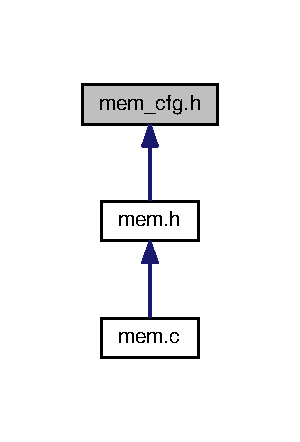
\includegraphics[width=144pt]{mem__cfg_8h__dep__incl}
\end{center}
\end{figure}
\subsubsection*{Macros}
\begin{Indent}{\bf e\-Solid memory allocator override}\par
\begin{DoxyCompactItemize}
\item 
\hypertarget{group__mem__cfg_ga543701ab60ff8b87e4e1ec9ea0b03491}{\#define {\bfseries O\-P\-T\-\_\-\-M\-E\-M\-\_\-\-A\-L\-L\-O\-C}~malloc}\label{group__mem__cfg_ga543701ab60ff8b87e4e1ec9ea0b03491}

\item 
\hypertarget{group__mem__cfg_gaab59d354bf34173761c3f95d0662c22e}{\#define {\bfseries O\-P\-T\-\_\-\-M\-E\-M\-\_\-\-F\-R\-E\-E}~free}\label{group__mem__cfg_gaab59d354bf34173761c3f95d0662c22e}

\end{DoxyCompactItemize}
\end{Indent}


\subsubsection{Detailed Description}
Konfiguracija memorijskog menadzmenta. \begin{DoxyAuthor}{Author}
Nenad Radulovic 
\end{DoxyAuthor}

\hypertarget{mem__example_8dox}{\subsection{mem\-\_\-example.\-dox File Reference}
\label{mem__example_8dox}\index{mem\-\_\-example.\-dox@{mem\-\_\-example.\-dox}}
}

\hypertarget{mem__mainpage_8dox}{\subsection{mem\-\_\-mainpage.\-dox File Reference}
\label{mem__mainpage_8dox}\index{mem\-\_\-mainpage.\-dox@{mem\-\_\-mainpage.\-dox}}
}

\section{Example Documentation}
\hypertarget{dmem_init1_8c-example}{\subsection{dmem\-\_\-init1.\-c}
}
This is an example how to initialize Dynamic Memory Manager. In this example a char buffer of B\-U\-F\-F\-E\-R\-\_\-\-S\-I\-Z\-E size is used to hold the data for Dynamic Memory Manager. B\-U\-F\-F\-E\-R\-\_\-\-S\-I\-Z\-E is set to 1024 so total buffer size is 1024 bytes. Keep in mind that Dynamic Memory Manager needs some parts of the buffer to keep track of its users so the available memory is slighty smaller then what is specified in B\-U\-F\-F\-E\-R\-\_\-\-S\-I\-Z\-E macro.


\begin{DoxyCodeInclude}
\textcolor{preprocessor}{#include "\hyperlink{mem_8h}{mem/mem.h}"}

\textcolor{preprocessor}{#define BUFFER\_SIZE                     1024}
\textcolor{preprocessor}{}
\textcolor{keywordtype}{int} main (
    \textcolor{keywordtype}{void}) \{

    \textcolor{keyword}{static} \textcolor{keywordtype}{char} buffer[BUFFER\_SIZE];
    \textcolor{keyword}{static} \hyperlink{structesDMemHandle}{esDMemHandle\_T} myHeap;

    \hyperlink{group__mem__intf_ga10ef80121c0c742b9ad81f24eff91c7f}{esDMemInit}(
        &myHeap,
        &buffer[0],
        \textcolor{keyword}{sizeof}(buffer));                                    \textcolor{comment}{/* Initialize the dynamic memory */}

    \textcolor{keywordflow}{while} (TRUE) \{
        \textcolor{keywordtype}{int} * myArray;

        myArray = \hyperlink{group__mem__intf_ga807a7d2e705b1802b7671c0c903611a6}{esDMemAllocI}(
            &myHeap,
            \textcolor{keyword}{sizeof}(\textcolor{keywordtype}{int}) * 10u);                             \textcolor{comment}{/* Allocate an array of 10 integers */}

        \textcolor{comment}{/*}
\textcolor{comment}{         * Do some stuff}
\textcolor{comment}{         */}

        \hyperlink{group__mem__intf_gad56192526f2b6ec1f927d21b15e1bc11}{esDMemDeAllocI}(
            &myHeap,
            myArray);                                       \textcolor{comment}{/* Delete the array */}
    \}
\}
\end{DoxyCodeInclude}
 
\hypertarget{dmem_init2_8c-example}{\subsection{dmem\-\_\-init2.\-c}
}
This is a more advanced example of Dynamic Memory initialization. First it initializes the static memory and requires 1024 bytes from it for data storage.


\begin{DoxyCodeInclude}
\textcolor{preprocessor}{#include "\hyperlink{mem_8h}{mem/mem.h}"}

\textcolor{preprocessor}{#define BUFFER\_SIZE                     1024}
\textcolor{preprocessor}{}
\textcolor{keywordtype}{int} main (
    \textcolor{keywordtype}{void}) \{

    \textcolor{keyword}{static} \hyperlink{structesPMemHandle}{esPMemHandle\_T} myBigStorage;
    \textcolor{keyword}{static} \textcolor{keywordtype}{char} myReallyBigStorage[16384];
    \textcolor{keyword}{static} \hyperlink{structesDMemHandle}{esDMemHandle\_T} myHeap;
    \textcolor{keyword}{static} \textcolor{keywordtype}{char} * buffer;

    \hyperlink{group__mem__intf_ga53acef4ba27e5e401ac2e1f862e07a8b}{esSMemInit}(
        &myBigStorage,
        &myReallyBigStorage[0],
        \textcolor{keyword}{sizeof}(myReallyBigStorage));                        \textcolor{comment}{/* Initialize the static memory */}

    buffer = \hyperlink{group__mem__intf_ga2e2086778aa0eb21156044730a1f380b}{esSMemAllocI}(
        BUFFER\_SIZE);                                       \textcolor{comment}{/* Allocate a buffer of 1024 bytes from static
       memory*/}

    \hyperlink{group__mem__intf_ga10ef80121c0c742b9ad81f24eff91c7f}{esDMemInit}(
        &myHeap,
        buffer,
        BUFFER\_SIZE);                                       \textcolor{comment}{/* Initialize the dynamic memory */}

    \textcolor{keywordflow}{while} (TRUE) \{
        \textcolor{keywordtype}{int} * myArray;

        myArray = \hyperlink{group__mem__intf_ga807a7d2e705b1802b7671c0c903611a6}{esDMemAllocI}(
            &myHeap,
            \textcolor{keyword}{sizeof}(\textcolor{keywordtype}{int}) * 10u);                             \textcolor{comment}{/* Allocate an array of 10 integers */}

        \textcolor{comment}{/*}
\textcolor{comment}{         * Do some stuff}
\textcolor{comment}{         */}

        \hyperlink{group__mem__intf_gad56192526f2b6ec1f927d21b15e1bc11}{esDMemDeAllocI}(
            &myHeap,
            myArray);                                       \textcolor{comment}{/* Delete the array */}
    \}
\}
\end{DoxyCodeInclude}
 
\hypertarget{dmem_two_buffs_8c-example}{\subsection{dmem\-\_\-two\-\_\-buffs.\-c}
}
In this example two independent Dynamic Memory buffers are created. Each buffer is used for its own purpose. This can have the benefit of reducing memory fragmentation. Lets say that the data needed to be saved is 40 bytes in size, while commands are only one integer in size. So by putting small data (commands) in one buffer and large data in other buffer the fragmentation can be reduced.


\begin{DoxyCodeInclude}
\textcolor{preprocessor}{#include "\hyperlink{mem_8h}{mem/mem.h}"}

\textcolor{preprocessor}{#define DATA\_BUFFER\_SIZE                2048}
\textcolor{preprocessor}{}\textcolor{preprocessor}{#define COMMAND\_BUFFER\_SIZE             512}
\textcolor{preprocessor}{}
\textcolor{keywordtype}{int} main (
    \textcolor{keywordtype}{void}) \{

    \textcolor{keyword}{static} \hyperlink{structesPMemHandle}{esPMemHandle\_T} myBigStorage;
    \textcolor{keyword}{static} \textcolor{keywordtype}{char} myReallyBigStorage[16384];
    \textcolor{keyword}{static} \hyperlink{structesDMemHandle}{esDMemHandle\_T} dataHeap;
    \textcolor{keyword}{static} \hyperlink{structesDMemHandle}{esDMemHandle\_T} commandHeap;
    \textcolor{keyword}{static} \textcolor{keywordtype}{char} * dataBuffer;
    \textcolor{keyword}{static} \textcolor{keywordtype}{char} * commandBuffer;

    \hyperlink{group__mem__intf_ga53acef4ba27e5e401ac2e1f862e07a8b}{esSMemInit}(
        &myBigStorage,
        &myReallyBigStorage[0],
        \textcolor{keyword}{sizeof}(myReallyBigStorage));                        \textcolor{comment}{/* Initialize the static memory */}

    dataBuffer = \hyperlink{group__mem__intf_ga2e2086778aa0eb21156044730a1f380b}{esSMemAllocI}(
        DATA\_BUFFER\_SIZE);                                  \textcolor{comment}{/* Create a data buffer of 2048 bytes */}
    commandBuffer = \hyperlink{group__mem__intf_ga2e2086778aa0eb21156044730a1f380b}{esSMemAllocI}(
        COMMAND\_BUFFER\_SIZE);                               \textcolor{comment}{/* Create additional buffer of 512 bytes */}

    \hyperlink{group__mem__intf_ga10ef80121c0c742b9ad81f24eff91c7f}{esDMemInit}(
        &dataHeap,
        dataBuffer,
        DATA\_BUFFER\_SIZE);                                  \textcolor{comment}{/* Initialize the dynamic memory for data */}

    \hyperlink{group__mem__intf_ga10ef80121c0c742b9ad81f24eff91c7f}{esDMemInit}(
        &commandHeap,
        commandBuffer,
        COMMAND\_BUFFER\_SIZE);                               \textcolor{comment}{/* Initialize the dynamic memory for commands 
      */}

    \textcolor{keywordflow}{while} (TRUE) \{
        \textcolor{keywordtype}{int} * data;
        \textcolor{keywordtype}{int} * command;

        data = \hyperlink{group__mem__intf_ga807a7d2e705b1802b7671c0c903611a6}{esDMemAllocI}(
            &dataHeap,
            \textcolor{keyword}{sizeof}(\textcolor{keywordtype}{int}) * 10u);                             \textcolor{comment}{/* Allocate an array of 10 integers */}

        command = \hyperlink{group__mem__intf_ga807a7d2e705b1802b7671c0c903611a6}{esDMemAllocI}(
            &commandHeap,
            \textcolor{keyword}{sizeof}(\textcolor{keywordtype}{int}));

        \textcolor{comment}{/*}
\textcolor{comment}{         * Do some stuff}
\textcolor{comment}{         */}

        \hyperlink{group__mem__intf_gad56192526f2b6ec1f927d21b15e1bc11}{esDMemDeAllocI}(
            &commandHeap,
            command);                                       \textcolor{comment}{/* Delete the command */}

        \hyperlink{group__mem__intf_gad56192526f2b6ec1f927d21b15e1bc11}{esDMemDeAllocI}(
            &dataHeap,
            data);                                          \textcolor{comment}{/* Delete the data */}
    \}
\}
\end{DoxyCodeInclude}
 
\hypertarget{pmem_init1_8c-example}{\subsection{pmem\-\_\-init1.\-c}
}
This example creates a memory pool which holds 10 data\-Block structures. The pool is referenced with my\-Pool handle, and all pool data is hold in pool\-Storage\mbox{[}\mbox{]} array. Before using the pool it must be first initialized by \hyperlink{group__mem__intf_gac151cf4385488838b0507936e67e2584}{es\-P\-Mem\-Init()} function. After initialization all pool memory functions can be used. Note that pool memory created here cannot be destroyed.


\begin{DoxyCodeInclude}
\textcolor{preprocessor}{#include <stdint.h>}
\textcolor{preprocessor}{#include "\hyperlink{mem_8h}{mem/mem.h}"}

\textcolor{keyword}{struct }dataBlock \{                                          \textcolor{comment}{/* Some application data structure*/}
    uint32\_t data01;
    uint32\_t data02;
    uint16\_t command;
\};

\textcolor{preprocessor}{#define POOL\_ELEMENTS                   10u                 }\textcolor{comment}{/* Specification of pool */}\textcolor{preprocessor}{}
\textcolor{preprocessor}{}
\textcolor{keywordtype}{int} main(
    \textcolor{keywordtype}{void}) \{

    \textcolor{keyword}{static} \hyperlink{structesPMemHandle}{esPMemHandle\_T} myPool;                           \textcolor{comment}{/* myPool pool handle */}
    \textcolor{keyword}{static} \textcolor{keyword}{struct }dataBlock poolStorage[POOL\_ELEMENTS];     \textcolor{comment}{/* pool storage */}

    \hyperlink{group__mem__intf_gac151cf4385488838b0507936e67e2584}{esPMemInit}(
        &myPool,
        &poolStorage,
        \textcolor{keyword}{sizeof}(poolStorage),
        \textcolor{keyword}{sizeof}(\textcolor{keyword}{struct} dataBlock));                          \textcolor{comment}{/* Initialize myPool pool memory */}

    \textcolor{keywordflow}{while} (TRUE) \{
        \textcolor{keyword}{struct }dataBlock * data;

        data = \hyperlink{group__mem__intf_gabdacce602565fcd6a186c2834cb74488}{esPMemAllocI}(
            &myPool);                                       \textcolor{comment}{/* Allocate a block from pool memory */}

        \textcolor{comment}{/*}
\textcolor{comment}{         * Do something}
\textcolor{comment}{         */}

        \hyperlink{group__mem__intf_ga2c0f1b135c5639809b17dfe44e06f1b5}{esPMemDeAllocI}(
            &myPool,
            data);                                          \textcolor{comment}{/* Return back the block */}
    \}
\}
\end{DoxyCodeInclude}
 
\hypertarget{pmem_init2_8c-example}{\subsection{pmem\-\_\-init2.\-c}
}
This example uses Static memory manager to allocate storage for pool memory. Before allocating the memory the required size of memory is calculated by following formula\-: sizeof(/\-Pool Element/) $\ast$ /\-Number of elements/. Use of E\-S\-\_\-\-A\-L\-I\-G\-N\-\_\-\-U\-P macro is highly recommended because all pool functions require that all data access is aligned. Static memory allocator always returns aligned value so there is no need to apply any alignment calculations on it.


\begin{DoxyCodeInclude}
\textcolor{preprocessor}{#include <stddef.h>}
\textcolor{preprocessor}{#include "\hyperlink{mem_8h}{mem/mem.h}"}

\textcolor{keyword}{struct }dataBlock \{                                          \textcolor{comment}{/* Some application data structure*/}
    uint32\_t data01;
    uint32\_t data02;
    uint16\_t command;
\};

\textcolor{preprocessor}{#define POOL\_ELEMENTS                   10u                 }\textcolor{comment}{/* Specification of pool */}\textcolor{preprocessor}{}
\textcolor{preprocessor}{}\textcolor{preprocessor}{#define POOL\_SIZE                       (ES\_BIT\_ALIGN\_UP(sizeof(struct dataBlock), sizeof(portReg\_T)) *
       POOL\_ELEMENTS)}
\textcolor{preprocessor}{}
\textcolor{keywordtype}{int} main(
    \textcolor{keywordtype}{void}) \{

    \textcolor{keyword}{static} \hyperlink{structesPMemHandle}{esPMemHandle\_T} myBigStorage;                     \textcolor{comment}{/* Static memory handle */}
    \textcolor{keyword}{static} \textcolor{keywordtype}{char} myReallyBigStorage[16384];                  \textcolor{comment}{/* Static memory storage */}
    \textcolor{keyword}{static} \hyperlink{structesPMemHandle}{esPMemHandle\_T} myPool;                           \textcolor{comment}{/* myPool pool handle */}
    \textcolor{keyword}{static} \textcolor{keywordtype}{void} * poolStorage;                              \textcolor{comment}{/* pointer to pool storage */}

    \hyperlink{group__mem__intf_ga53acef4ba27e5e401ac2e1f862e07a8b}{esSMemInit}(
        &myBigStorage,
        &myReallyBigStorage[0],
        \textcolor{keyword}{sizeof}(myReallyBigStorage));                        \textcolor{comment}{/* Initialize the static memory */}

    poolStorage = \hyperlink{group__mem__intf_ga2e2086778aa0eb21156044730a1f380b}{esSMemAllocI}(
        POOL\_SIZE);                                         \textcolor{comment}{/* Allocate pool storage memory */}
    \hyperlink{group__mem__intf_gac151cf4385488838b0507936e67e2584}{esPMemInit}(
        &myPool,
        poolStorage,
        POOL\_SIZE,
        ES\_BIT\_ALIGN\_UP(\textcolor{keyword}{sizeof}(\textcolor{keyword}{struct} dataBlock), \textcolor{keyword}{sizeof}(portReg\_T))); \textcolor{comment}{/* Initialize myPool pool memory */}

    \textcolor{keywordflow}{while} (TRUE) \{
        \textcolor{keyword}{struct }dataBlock * data;

        data = \hyperlink{group__mem__intf_gabdacce602565fcd6a186c2834cb74488}{esPMemAllocI}(
            &myPool);                                       \textcolor{comment}{/* Allocate a block from pool memory */}

        \textcolor{comment}{/*}
\textcolor{comment}{         * Do something}
\textcolor{comment}{         */}

        \hyperlink{group__mem__intf_ga2c0f1b135c5639809b17dfe44e06f1b5}{esPMemDeAllocI}(
            &myPool,
            data);                                          \textcolor{comment}{/* Return back the block */}
    \}
\}
\end{DoxyCodeInclude}
 
\hypertarget{pmem_init3_8c-example}{\subsection{pmem\-\_\-init3.\-c}
}
This example is very similar to pmem\-\_\-init2.\-c. The only difference is how the required pool storage size is calculated.


\begin{DoxyCodeInclude}
\textcolor{preprocessor}{#include <stddef.h>}
\textcolor{preprocessor}{#include <stdint.h>}
\textcolor{preprocessor}{#include "\hyperlink{mem_8h}{mem/mem.h}"}

\textcolor{keyword}{struct }dataBlock \{                                          \textcolor{comment}{/* Some application data structure which will
       be placed in pool */}
    uint32\_t data01;
    uint32\_t data02;
    uint16\_t command;
\};

\textcolor{preprocessor}{#define POOL\_ELEMENTS                   10u                 }\textcolor{comment}{/* Number of blocks in the pool */}\textcolor{preprocessor}{}
\textcolor{preprocessor}{}
\textcolor{keywordtype}{int} main(
    \textcolor{keywordtype}{void}) \{

    \textcolor{keyword}{static} \hyperlink{structesPMemHandle}{esPMemHandle\_T} myBigStorage;
    \textcolor{keyword}{static} \textcolor{keywordtype}{char} myReallyBigStorage[16384];
    \textcolor{keyword}{static} \hyperlink{structesPMemHandle}{esPMemHandle\_T} myPool;                           \textcolor{comment}{/* myPool pool handle */}
    \textcolor{keyword}{static} \textcolor{keywordtype}{void} * poolStorage;                              \textcolor{comment}{/* pointer to pool storage */}
    \textcolor{keyword}{static} \textcolor{keywordtype}{size\_t} poolSize;                                 \textcolor{comment}{/* size of pool */}

    \hyperlink{group__mem__intf_ga53acef4ba27e5e401ac2e1f862e07a8b}{esSMemInit}(
        &myBigStorage,
        &myReallyBigStorage[0],
        \textcolor{keyword}{sizeof}(myReallyBigStorage));                        \textcolor{comment}{/* Initialize the static memory */}

    poolSize = \hyperlink{group__mem__intf_gab82743b6c82847c748bf5193f0f211ec}{esPMemCalcPoolSize}(
        \textcolor{keyword}{sizeof}(\textcolor{keyword}{struct} dataBlock),
        POOL\_ELEMENTS);                                     \textcolor{comment}{/* Calculate the required pool size which will
       hold */}
                                                            \textcolor{comment}{/* POOL\_ELEMENTS number of structures of type
       dataBlock */}
    poolStorage = \hyperlink{group__mem__intf_ga2e2086778aa0eb21156044730a1f380b}{esSMemAllocI}(
        poolSize);                                          \textcolor{comment}{/* Allocate pool storage memory */}
    \hyperlink{group__mem__intf_gac151cf4385488838b0507936e67e2584}{esPMemInit}(
        &myPool,
        poolStorage,
        poolSize,
        \textcolor{keyword}{sizeof}(\textcolor{keyword}{struct} dataBlock));                          \textcolor{comment}{/* Initialize myPool pool memory */}

    \textcolor{keywordflow}{while} (TRUE) \{
        \textcolor{keyword}{struct }dataBlock * data;

        data = \hyperlink{group__mem__intf_gabdacce602565fcd6a186c2834cb74488}{esPMemAllocI}(
            &myPool);                                       \textcolor{comment}{/* Allocate a block from pool memory */}

        \textcolor{comment}{/*}
\textcolor{comment}{         * Do something with data}
\textcolor{comment}{         */}

        \hyperlink{group__mem__intf_ga2c0f1b135c5639809b17dfe44e06f1b5}{esPMemDeAllocI}(
            &myPool,
            data);                                          \textcolor{comment}{/* Return back the block */}
    \}
\}
\end{DoxyCodeInclude}
 
\hypertarget{pmem_two_buffs_8c-example}{\subsection{pmem\-\_\-two\-\_\-buffs.\-c}
}
T\-O\-D\-O


\begin{DoxyCodeInclude}
\textcolor{preprocessor}{#include <stdint.h>}
\textcolor{preprocessor}{#include "\hyperlink{mem_8h}{mem/mem.h}"}

\textcolor{preprocessor}{#define DATA\_ELEMENTS                   200u                }\textcolor{comment}{/* Number of blocks in data pool */}\textcolor{preprocessor}{}
\textcolor{preprocessor}{}\textcolor{preprocessor}{#define COMMAND\_ELEMENTS                100u                }\textcolor{comment}{/* Number of blocks in command pool */}\textcolor{preprocessor}{}
\textcolor{preprocessor}{}
\textcolor{keyword}{struct }dataElement \{                                        \textcolor{comment}{/* A sample structure representing application
       data */}
    uint32\_t data01;
    uint32\_t data02;
\};

\textcolor{keywordtype}{int} main (
    \textcolor{keywordtype}{void}) \{

    \textcolor{keyword}{static} \hyperlink{structesPMemHandle}{esPMemHandle\_T} dataPool;
    \textcolor{keyword}{static} \hyperlink{structesPMemHandle}{esPMemHandle\_T} commandPool;
    \textcolor{keyword}{static} \textcolor{keyword}{struct }dataElement dataStorage[DATA\_ELEMENTS];   \textcolor{comment}{/* This will hold application data */}
    \textcolor{keyword}{static} \textcolor{keywordtype}{int} commandStorage[COMMAND\_ELEMENTS];            \textcolor{comment}{/* This will hold application commands, each
       command is one integer */}

    \hyperlink{group__mem__intf_gac151cf4385488838b0507936e67e2584}{esPMemInit}(
        &dataPool,
        &dataStorage,
        \textcolor{keyword}{sizeof}(dataStorage),
        \textcolor{keyword}{sizeof}(\textcolor{keyword}{struct} dataElement));                        \textcolor{comment}{/* Initialize the pool memory for data */}

    \hyperlink{group__mem__intf_gac151cf4385488838b0507936e67e2584}{esPMemInit}(
        &commandPool,
        &commandStorage,
        \textcolor{keyword}{sizeof}(commandStorage),
        \textcolor{keyword}{sizeof}(\textcolor{keywordtype}{int}));                                       \textcolor{comment}{/* Initialize the pool memory for commands */}

    \textcolor{keywordflow}{while} (TRUE) \{
        \textcolor{keywordtype}{int} * data;
        \textcolor{keywordtype}{int} * command;

        data = \hyperlink{group__mem__intf_gabdacce602565fcd6a186c2834cb74488}{esPMemAllocI}(
            &dataPool);                                     \textcolor{comment}{/* Allocate memory for data */}

        command = \hyperlink{group__mem__intf_gabdacce602565fcd6a186c2834cb74488}{esPMemAllocI}(
            &commandPool);                                  \textcolor{comment}{/* Allocate memory for command */}

        \textcolor{comment}{/*}
\textcolor{comment}{         * Do some stuff}
\textcolor{comment}{         */}

        \hyperlink{group__mem__intf_ga2c0f1b135c5639809b17dfe44e06f1b5}{esPMemDeAllocI}(
            &commandPool,
            command);                                       \textcolor{comment}{/* Delete the command */}

        \hyperlink{group__mem__intf_ga2c0f1b135c5639809b17dfe44e06f1b5}{esPMemDeAllocI}(
            &dataPool,
            data);                                          \textcolor{comment}{/* Delete the data */}
    \}
\}
\end{DoxyCodeInclude}
 
%--- End generated contents ---

% Index
\newpage
\phantomsection
\addcontentsline{toc}{part}{Index}
\printindex

\end{document}
